\documentclass{whiteboard}
\begin{document}
\begin{frame}[plain,t]
\bbcover{Grafos}{Ancestrais}{Prof. Edson Alves}{Faculdade UnB Gama}

\end{frame}
\begin{frame}[plain,t]
\begin{tikzpicture}
\node[draw,opacity=0] at (0, 0) {x};
\node[draw,opacity=0] at (14, 8) {x};

	\node[anchor=west] (title) at (0.0, 6.5) { \Large \bbbold{$k$-ésimo ancestral} };

	\node[anchor=west] (a) at (1.0, 5.5) { \bbtext{Seja $T$ uma árvore enraizada, $u$ um vértice de $T$ e $k$ um inteiro positivo.} };

	\node[anchor=west] (b) at (0.5, 4.75) { \bbtext{O $k$-\bbbold{ésimo ancestral de} $u$ é o nó $v$ que encerra o caminho que parte de $u$ e} };

	\node[anchor=west] (c) at (0.5, 4.0) { \bbtext{segue $k$ níveis, em direção à raiz. \bbbold{Notação:} \texttt{$v$ = ancestor(}$u, k$\texttt{)}.} };

\end{tikzpicture}
\end{frame}
\begin{frame}[plain,t]
\begin{tikzpicture}
\node[draw,opacity=0] at (0, 0) {x};
\node[draw,opacity=0] at (14, 8) {x};

	\node[very thick,draw,circle] (node1) at (9.0, 3.0) { \bbtext{1} };

	\node[very thick,draw,circle] (node2) at (9.0, 5.0) { \bbtext{2} };

	\node[very thick,draw,circle] (node3) at (5.0, 7.0) { \bbtext{3} };

	\node[very thick,draw,circle] (node4) at (5.0, 5.0) { \bbtext{4} };

	\node[very thick,draw,circle] (node5) at (9.0, 1.0) { \bbtext{5} };

	\node[very thick,draw,circle] (node7) at (1.0, 5.0) { \bbtext{7} };

	\node[very thick,draw,circle] (node6) at (6.0, 3.0) { \bbtext{6} };

	\node[very thick,draw,circle] (node8) at (12.0, 3.0) { \bbtext{8} };

	\node[very thick,draw,circle] (node9) at (1.0, 3.0) { \bbtext{9} };


	\draw[thick](node1) to (node2);

	\draw[thick](node1) to (node5);

	\draw[thick](node3) to (node2);

	\draw[thick](node6) to (node2);

	\draw[thick](node8) to (node2);

	\draw[thick](node2) to (node3);

	\draw[thick](node3) to (node4);

	\draw[thick](node3) to (node7);

	\draw[thick](node7) to (node9);

\end{tikzpicture}
\end{frame}
\begin{frame}[plain,t]
\begin{tikzpicture}
\node[draw,opacity=0] at (0, 0) {x};
\node[draw,opacity=0] at (14, 8) {x};

	\node[very thick,draw,circle] (node1) at (9.0, 3.0) { \bbtext{1} };

	\node[very thick,draw,circle] (node2) at (9.0, 5.0) { \bbtext{2} };

	\node[very thick,draw,circle] (node3) at (5.0, 7.0) { \bbtext{3} };

	\node[very thick,draw,circle] (node4) at (5.0, 5.0) { \bbtext{4} };

	\node[very thick,draw,circle] (node5) at (9.0, 1.0) { \bbtext{5} };

	\node[very thick,draw,circle] (node7) at (1.0, 5.0) { \bbtext{7} };

	\node[very thick,draw,circle] (node6) at (6.0, 3.0) { \bbtext{6} };

	\node[very thick,draw,circle] (node8) at (12.0, 3.0) { \bbtext{8} };

	\node[very thick,draw,circle] (node9) at (1.0, 3.0) { \bbtext{9} };


	\draw[thick](node1) to (node2);

	\draw[thick](node1) to (node5);

	\draw[thick](node3) to (node2);

	\draw[thick](node6) to (node2);

	\draw[thick](node8) to (node2);

	\draw[thick](node2) to (node3);

	\draw[thick](node3) to (node4);

	\draw[thick](node3) to (node7);

	\draw[thick](node7) to (node9);


	\draw[color=BBViolet,thick,-latex,dashed](node9) to [bend right] node[anchor=west] { \scriptsize \texttt{ancestor($9, 1$) = 7} } (node7);

\end{tikzpicture}
\end{frame}
\begin{frame}[plain,t]
\begin{tikzpicture}
\node[draw,opacity=0] at (0, 0) {x};
\node[draw,opacity=0] at (14, 8) {x};

	\node[very thick,draw,circle] (node1) at (9.0, 3.0) { \bbtext{1} };

	\node[very thick,draw,circle] (node2) at (9.0, 5.0) { \bbtext{2} };

	\node[very thick,draw,circle] (node3) at (5.0, 7.0) { \bbtext{3} };

	\node[very thick,draw,circle] (node4) at (5.0, 5.0) { \bbtext{4} };

	\node[very thick,draw,circle] (node5) at (9.0, 1.0) { \bbtext{5} };

	\node[very thick,draw,circle] (node7) at (1.0, 5.0) { \bbtext{7} };

	\node[very thick,draw,circle] (node6) at (6.0, 3.0) { \bbtext{6} };

	\node[very thick,draw,circle] (node8) at (12.0, 3.0) { \bbtext{8} };

	\node[very thick,draw,circle] (node9) at (1.0, 3.0) { \bbtext{9} };


	\draw[thick](node1) to (node2);

	\draw[thick](node1) to (node5);

	\draw[thick](node3) to (node2);

	\draw[thick](node6) to (node2);

	\draw[thick](node8) to (node2);

	\draw[thick](node2) to (node3);

	\draw[thick](node3) to (node4);

	\draw[thick](node3) to (node7);

	\draw[thick](node7) to (node9);


	\draw[color=BBViolet,thick,-latex,dashed](node9) to [bend right] node[anchor=west] { \scriptsize \texttt{ancestor($9, 1$) = 7} } (node7);


	\draw[color=BBGreen,thick,-latex,dashed](node6) to [bend right] (node2);

	\draw[color=BBGreen,thick,-latex,dashed](node2) to [bend right] node[anchor=south west] { \scriptsize \texttt{ancestor($6, 2$) = 3} } (node3);

\end{tikzpicture}
\end{frame}
\begin{frame}[plain,t]
\begin{tikzpicture}
\node[draw,opacity=0] at (0, 0) {x};
\node[draw,opacity=0] at (14, 8) {x};

	\node[very thick,draw,circle] (node1) at (9.0, 3.0) { \bbtext{1} };

	\node[very thick,draw,circle] (node2) at (9.0, 5.0) { \bbtext{2} };

	\node[very thick,draw,circle] (node3) at (5.0, 7.0) { \bbtext{3} };

	\node[very thick,draw,circle] (node4) at (5.0, 5.0) { \bbtext{4} };

	\node[very thick,draw,circle] (node5) at (9.0, 1.0) { \bbtext{5} };

	\node[very thick,draw,circle] (node7) at (1.0, 5.0) { \bbtext{7} };

	\node[very thick,draw,circle] (node6) at (6.0, 3.0) { \bbtext{6} };

	\node[very thick,draw,circle] (node8) at (12.0, 3.0) { \bbtext{8} };

	\node[very thick,draw,circle] (node9) at (1.0, 3.0) { \bbtext{9} };


	\draw[thick](node1) to (node2);

	\draw[thick](node1) to (node5);

	\draw[thick](node3) to (node2);

	\draw[thick](node6) to (node2);

	\draw[thick](node8) to (node2);

	\draw[thick,color=BBCyan,-latex,dashed](node2) to [bend left] (node3);

	\draw[thick](node3) to (node4);

	\draw[thick](node3) to (node7);

	\draw[thick](node7) to (node9);


	\draw[color=BBViolet,thick,-latex,dashed](node9) to [bend right] node[anchor=west] { \scriptsize \texttt{ancestor($9, 1$) = 7} } (node7);


	\draw[color=BBGreen,thick,-latex,dashed](node6) to [bend right] (node2);

	\draw[color=BBGreen,thick,-latex,dashed](node2) to [bend right] node[anchor=south west] { \scriptsize \texttt{ancestor($6, 2$) = 3} } (node3);


	\draw[color=BBCyan,thick,-latex,dashed](node5) to [bend right] node[anchor=west] { \scriptsize \texttt{ancestor($5, 3$) = 3} } (node1);

	\draw[color=BBCyan,thick,-latex,dashed](node1) to [bend right] (node2);

	\draw[color=BBCyan,thick,-latex,dashed](node2) to [bend left] (node3);


\end{tikzpicture}
\end{frame}
\begin{frame}[plain,t]
\begin{tikzpicture}
\node[draw,opacity=0] at (0, 0) {x};
\node[draw,opacity=0] at (14, 8) {x};

	\node[anchor=west] (title) at (0.0, 7.0) { \Large \bbbold{Identificação do $k$-eśimo ancestral em $O(\log N)$} };

\end{tikzpicture}
\end{frame}
\begin{frame}[plain,t]
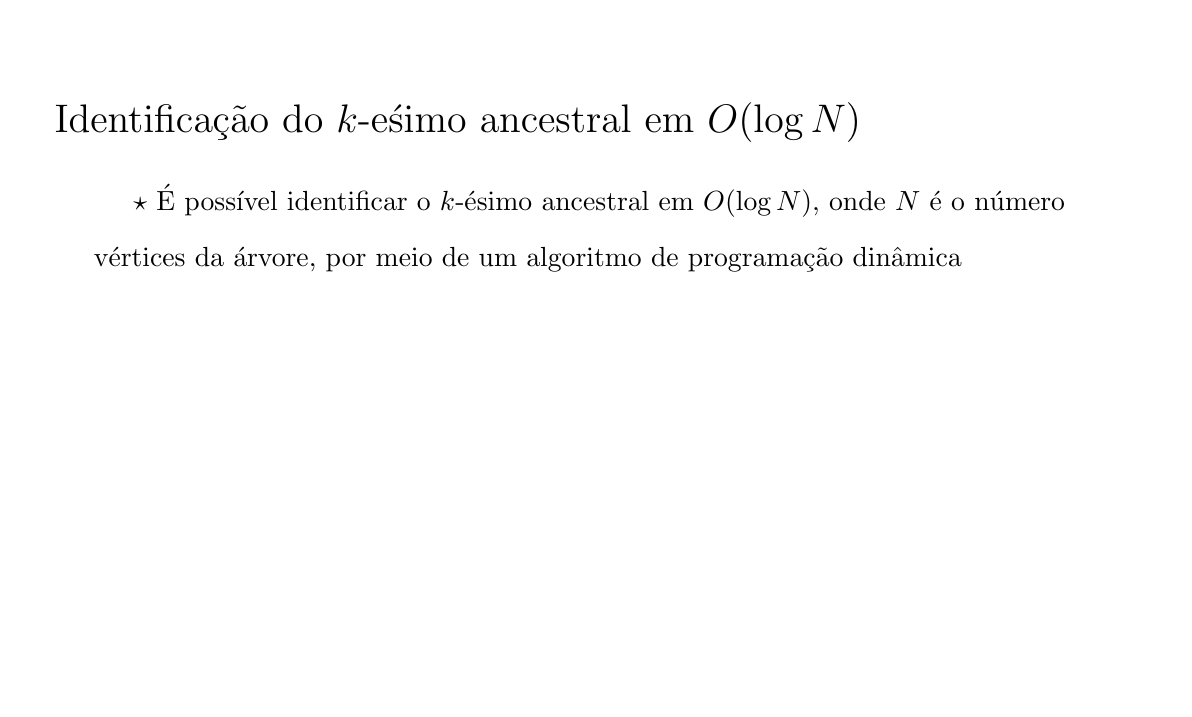
\begin{tikzpicture}
\node[draw,opacity=0] at (0, 0) {x};
\node[draw,opacity=0] at (14, 8) {x};

	\node[anchor=west] (title) at (0.0, 7.0) { \Large \bbbold{Identificação do $k$-eśimo ancestral em $O(\log N)$} };


	\node[anchor=west] (a) at (1.0, 6.0) { $\star$ \bbtext{É possível identificar o $k$-ésimo ancestral em $O(\log N)$, onde $N$ é o número} };

	\node[anchor=west] (a1) at (0.5, 5.25) { \bbtext{vértices da árvore, por meio de um algoritmo de programação dinâmica} };

\end{tikzpicture}
\end{frame}
\begin{frame}[plain,t]
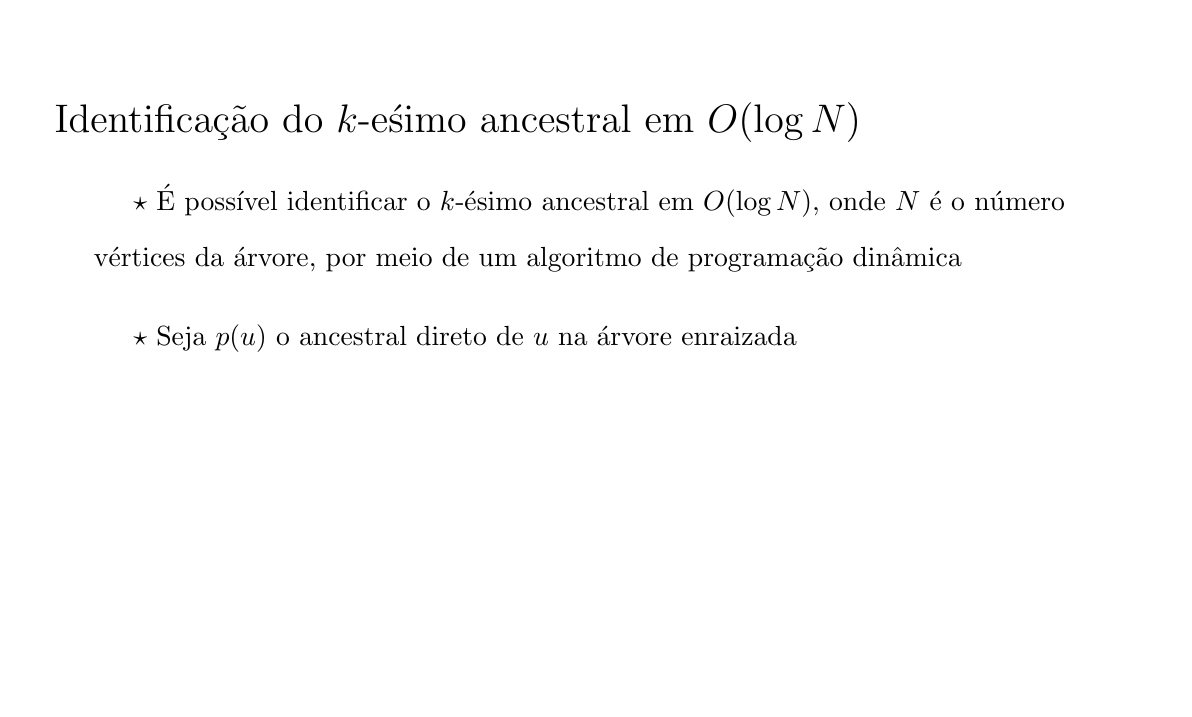
\begin{tikzpicture}
\node[draw,opacity=0] at (0, 0) {x};
\node[draw,opacity=0] at (14, 8) {x};

	\node[anchor=west] (title) at (0.0, 7.0) { \Large \bbbold{Identificação do $k$-eśimo ancestral em $O(\log N)$} };


	\node[anchor=west] (a) at (1.0, 6.0) { $\star$ \bbtext{É possível identificar o $k$-ésimo ancestral em $O(\log N)$, onde $N$ é o número} };

	\node[anchor=west] (a1) at (0.5, 5.25) { \bbtext{vértices da árvore, por meio de um algoritmo de programação dinâmica} };


	\node[anchor=west] (b) at (1.0, 4.25) { $\star$ \bbtext{Seja $p(u)$ o ancestral direto de $u$ na árvore enraizada} };


\end{tikzpicture}
\end{frame}
\begin{frame}[plain,t]
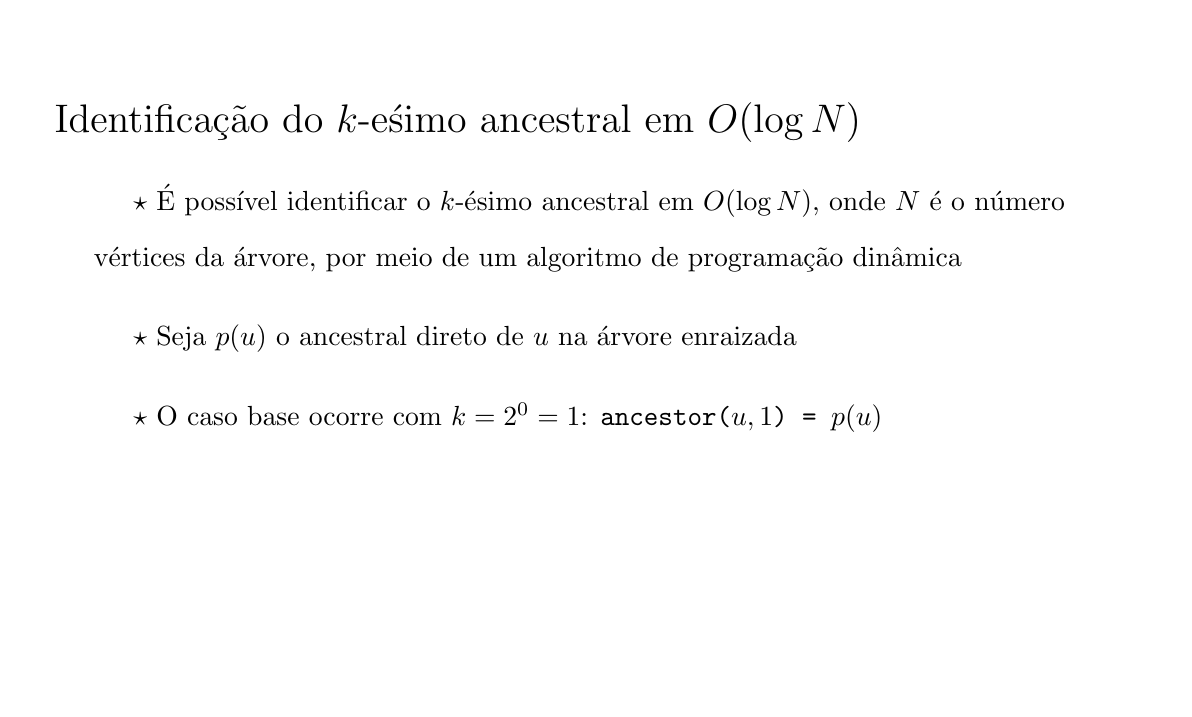
\begin{tikzpicture}
\node[draw,opacity=0] at (0, 0) {x};
\node[draw,opacity=0] at (14, 8) {x};

	\node[anchor=west] (title) at (0.0, 7.0) { \Large \bbbold{Identificação do $k$-eśimo ancestral em $O(\log N)$} };


	\node[anchor=west] (a) at (1.0, 6.0) { $\star$ \bbtext{É possível identificar o $k$-ésimo ancestral em $O(\log N)$, onde $N$ é o número} };

	\node[anchor=west] (a1) at (0.5, 5.25) { \bbtext{vértices da árvore, por meio de um algoritmo de programação dinâmica} };


	\node[anchor=west] (b) at (1.0, 4.25) { $\star$ \bbtext{Seja $p(u)$ o ancestral direto de $u$ na árvore enraizada} };



	\node[anchor=west] (c) at (1.0, 3.25) { $\star$ \bbtext{O caso base ocorre com $k = 2^0 = 1$:  \texttt{ancestor($u, 1$) = $p(u)$}} };

\end{tikzpicture}
\end{frame}
\begin{frame}[plain,t]
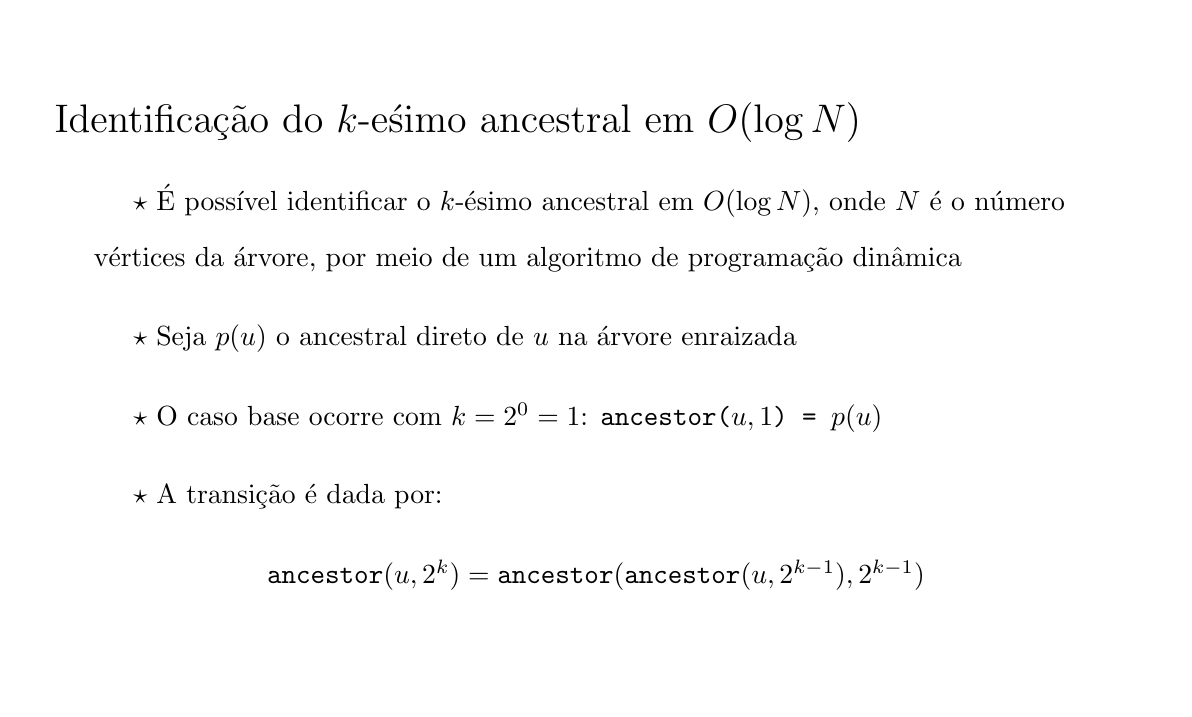
\begin{tikzpicture}
\node[draw,opacity=0] at (0, 0) {x};
\node[draw,opacity=0] at (14, 8) {x};

	\node[anchor=west] (title) at (0.0, 7.0) { \Large \bbbold{Identificação do $k$-eśimo ancestral em $O(\log N)$} };


	\node[anchor=west] (a) at (1.0, 6.0) { $\star$ \bbtext{É possível identificar o $k$-ésimo ancestral em $O(\log N)$, onde $N$ é o número} };

	\node[anchor=west] (a1) at (0.5, 5.25) { \bbtext{vértices da árvore, por meio de um algoritmo de programação dinâmica} };


	\node[anchor=west] (b) at (1.0, 4.25) { $\star$ \bbtext{Seja $p(u)$ o ancestral direto de $u$ na árvore enraizada} };



	\node[anchor=west] (c) at (1.0, 3.25) { $\star$ \bbtext{O caso base ocorre com $k = 2^0 = 1$:  \texttt{ancestor($u, 1$) = $p(u)$}} };


	\node[anchor=west] (d) at (1.0, 2.25) { $\star$ \bbtext{A transição é dada por:} };

	\node[] (d1) at (7.0, 1.25) { $ \texttt{ancestor}(u, 2^k) = \texttt{ancestor}(\texttt{ancestor}(u, 2^{k - 1}), 2^{k - 1}) $ };

\end{tikzpicture}
\end{frame}
\begin{frame}[plain,t]
\begin{tikzpicture}
\node[draw,opacity=0] at (0, 0) {x};
\node[draw,opacity=0] at (14, 8) {x};

	\node[anchor=west] (title) at (0.0, 7.0) { \Large \bbbold{Identificação do $k$-eśimo ancestral em $O(\log N)$} };

\end{tikzpicture}
\end{frame}
\begin{frame}[plain,t]
\begin{tikzpicture}
\node[draw,opacity=0] at (0, 0) {x};
\node[draw,opacity=0] at (14, 8) {x};

	\node[anchor=west] (title) at (0.0, 7.0) { \Large \bbbold{Identificação do $k$-eśimo ancestral em $O(\log N)$} };


	\node[anchor=west] (a) at (1.0, 6.0) { $\star$ \bbtext{Seja $k$ um inteiro positivo} };

\end{tikzpicture}
\end{frame}
\begin{frame}[plain,t]
\begin{tikzpicture}
\node[draw,opacity=0] at (0, 0) {x};
\node[draw,opacity=0] at (14, 8) {x};

	\node[anchor=west] (title) at (0.0, 7.0) { \Large \bbbold{Identificação do $k$-eśimo ancestral em $O(\log N)$} };


	\node[anchor=west] (a) at (1.0, 6.0) { $\star$ \bbtext{Seja $k$ um inteiro positivo} };


	\node[anchor=west] (b) at (1.0, 5.0) { $\star$ \bbtext{É possível escrever $k$ como a soma de potências distintas de $2$:} };

	\node[] (b1) at (7.0, 4.0) { $k = 2^{\alpha} + 2^{\beta} + \ldots + 2^{\omega}$ };

\end{tikzpicture}
\end{frame}
\begin{frame}[plain,t]
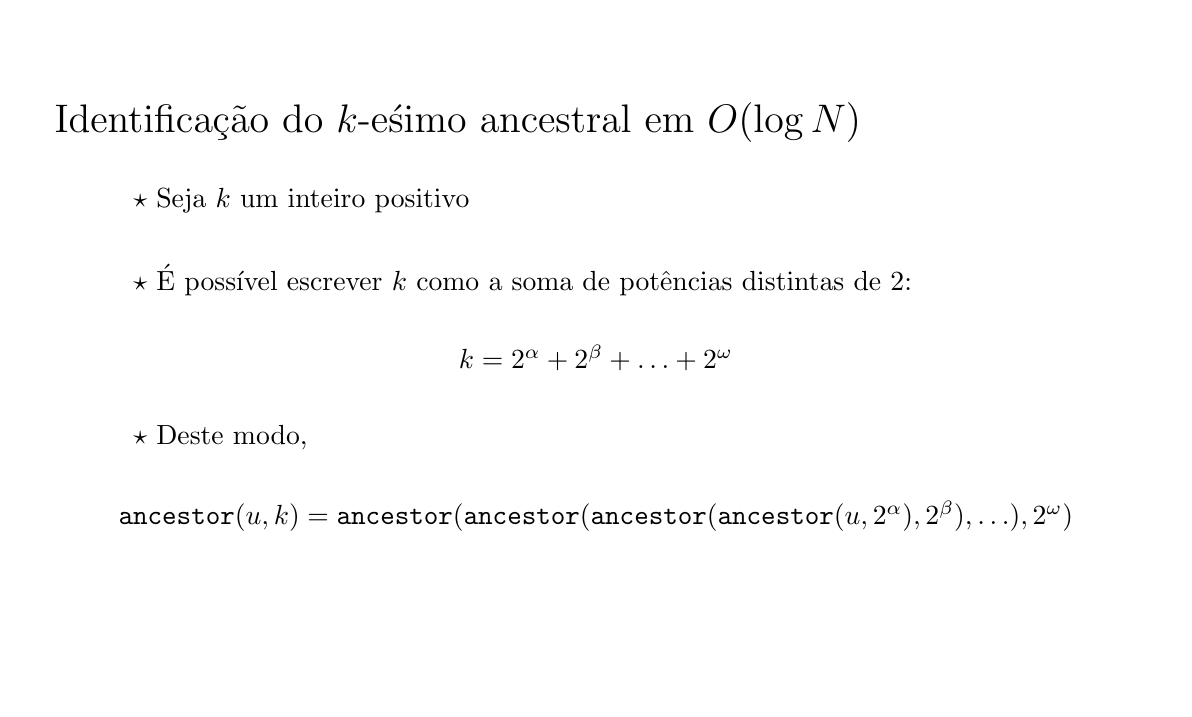
\begin{tikzpicture}
\node[draw,opacity=0] at (0, 0) {x};
\node[draw,opacity=0] at (14, 8) {x};

	\node[anchor=west] (title) at (0.0, 7.0) { \Large \bbbold{Identificação do $k$-eśimo ancestral em $O(\log N)$} };


	\node[anchor=west] (a) at (1.0, 6.0) { $\star$ \bbtext{Seja $k$ um inteiro positivo} };


	\node[anchor=west] (b) at (1.0, 5.0) { $\star$ \bbtext{É possível escrever $k$ como a soma de potências distintas de $2$:} };

	\node[] (b1) at (7.0, 4.0) { $k = 2^{\alpha} + 2^{\beta} + \ldots + 2^{\omega}$ };


	\node[anchor=west] (c) at (1.0, 3.0) { $\star$ \bbtext{Deste modo,} };

	\node[] (c1) at (7.0, 2.0) { $\texttt{ancestor}(u, k) =  \texttt{ancestor}(\texttt{ancestor}(\texttt{ancestor}(\texttt{ancestor}(u, 2^\alpha), 2^\beta), \ldots), 2^\omega)$ };


\end{tikzpicture}
\end{frame}
\begin{frame}[plain,t]
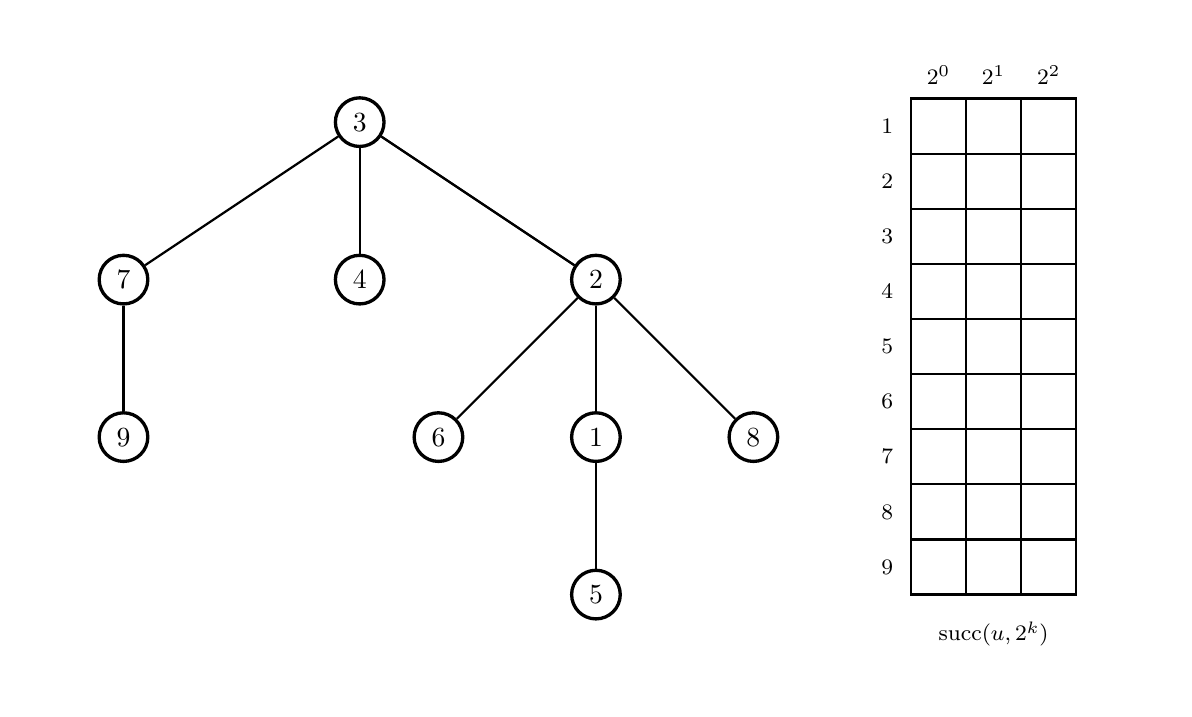
\begin{tikzpicture}
\node[draw,opacity=0] at (0, 0) {x};
\node[draw,opacity=0] at (14, 8) {x};

	\node[very thick,draw,circle] (node1) at (7.0, 3.0) { \bbtext{1} };

	\node[very thick,draw,circle] (node2) at (7.0, 5.0) { \bbtext{2} };

	\node[very thick,draw,circle] (node3) at (4.0, 7.0) { \bbtext{3} };

	\node[very thick,draw,circle] (node4) at (4.0, 5.0) { \bbtext{4} };

	\node[very thick,draw,circle] (node5) at (7.0, 1.0) { \bbtext{5} };

	\node[very thick,draw,circle] (node7) at (1.0, 5.0) { \bbtext{7} };

	\node[very thick,draw,circle] (node6) at (5.0, 3.0) { \bbtext{6} };

	\node[very thick,draw,circle] (node8) at (9.0, 3.0) { \bbtext{8} };

	\node[very thick,draw,circle] (node9) at (1.0, 3.0) { \bbtext{9} };


	\draw[thick](node1) to (node2);

	\draw[thick](node1) to (node5);

	\draw[thick](node3) to (node2);

	\draw[thick](node6) to (node2);

	\draw[thick](node8) to (node2);

	\draw[thick](node2) to (node3);

	\draw[thick](node3) to (node4);

	\draw[thick](node3) to (node7);

	\draw[thick](node7) to (node9);

	\draw[thick] (11, 7.3) -- (13.1, 7.3) -- (13.1, 1) -- (11, 1) -- cycle;

	\draw[thick] (11.7, 7.3) -- (11.7, 1);

	\draw[thick] (12.4, 7.3) -- (12.4, 1);

	\draw[thick] (11, 6.6) -- (13.1, 6.6);

	\draw[thick] (11, 5.9) -- (13.1, 5.9);

	\draw[thick] (11, 5.2) -- (13.1, 5.2);

	\draw[thick] (11, 4.5) -- (13.1, 4.5);

	\draw[thick] (11, 3.8) -- (13.1, 3.8);

	\draw[thick] (11, 3.1) -- (13.1, 3.1);

	\draw[thick] (11, 2.4) -- (13.1, 2.4);

	\draw[thick] (11, 1.7) -- (13.1, 1.7);

	\node[] (k1) at (11.35, 7.6) { \footnotesize $2^0$ };

	\node[] (k2) at (12.05, 7.6) { \footnotesize $2^1$ };

	\node[] (k3) at (12.75, 7.6) { \footnotesize $2^2$ };

	\node[] (x1) at (10.7, 6.95) { \footnotesize \bbtext{1} };

	\node[] (x2) at (10.7, 6.25) { \footnotesize \bbtext{2} };

	\node[] (x3) at (10.7, 5.55) { \footnotesize \bbtext{3} };

	\node[] (x4) at (10.7, 4.85) { \footnotesize \bbtext{4} };

	\node[] (x5) at (10.7, 4.15) { \footnotesize \bbtext{5} };

	\node[] (x6) at (10.7, 3.45) { \footnotesize \bbtext{6} };

	\node[] (x7) at (10.7, 2.75) { \footnotesize \bbtext{7} };

	\node[] (x8) at (10.7, 2.05) { \footnotesize \bbtext{8} };

	\node[] (x9) at (10.7, 1.35) { \footnotesize \bbtext{9} };

	\node[] (succ) at (12.05, 0.5) { \footnotesize $\mathrm{succ}(u, 2^k)$ };

\end{tikzpicture}
\end{frame}
\begin{frame}[plain,t]
\begin{tikzpicture}
\node[draw,opacity=0] at (0, 0) {x};
\node[draw,opacity=0] at (14, 8) {x};

	\node[very thick,draw,circle,fill=BBCyan] (node1) at (7.0, 3.0) { \bbtext{1} };

	\node[very thick,draw,circle] (node2) at (7.0, 5.0) { \bbtext{2} };

	\node[very thick,draw,circle] (node3) at (4.0, 7.0) { \bbtext{3} };

	\node[very thick,draw,circle] (node4) at (4.0, 5.0) { \bbtext{4} };

	\node[very thick,draw,circle] (node5) at (7.0, 1.0) { \bbtext{5} };

	\node[very thick,draw,circle] (node7) at (1.0, 5.0) { \bbtext{7} };

	\node[very thick,draw,circle] (node6) at (5.0, 3.0) { \bbtext{6} };

	\node[very thick,draw,circle] (node8) at (9.0, 3.0) { \bbtext{8} };

	\node[very thick,draw,circle] (node9) at (1.0, 3.0) { \bbtext{9} };


	\draw[thick](node1) to (node2);

	\draw[thick](node1) to (node5);

	\draw[thick](node3) to (node2);

	\draw[thick](node6) to (node2);

	\draw[thick](node8) to (node2);

	\draw[thick](node2) to (node3);

	\draw[thick](node3) to (node4);

	\draw[thick](node3) to (node7);

	\draw[thick](node7) to (node9);

	\draw[thick] (11, 7.3) -- (13.1, 7.3) -- (13.1, 1) -- (11, 1) -- cycle;

	\draw[thick] (11.7, 7.3) -- (11.7, 1);

	\draw[thick] (12.4, 7.3) -- (12.4, 1);

	\draw[thick] (11, 6.6) -- (13.1, 6.6);

	\draw[thick] (11, 5.9) -- (13.1, 5.9);

	\draw[thick] (11, 5.2) -- (13.1, 5.2);

	\draw[thick] (11, 4.5) -- (13.1, 4.5);

	\draw[thick] (11, 3.8) -- (13.1, 3.8);

	\draw[thick] (11, 3.1) -- (13.1, 3.1);

	\draw[thick] (11, 2.4) -- (13.1, 2.4);

	\draw[thick] (11, 1.7) -- (13.1, 1.7);

	\node[] (k1) at (11.35, 7.6) { \footnotesize $2^0$ };

	\node[] (k2) at (12.05, 7.6) { \footnotesize $2^1$ };

	\node[] (k3) at (12.75, 7.6) { \footnotesize $2^2$ };

	\node[] (x1) at (10.7, 6.95) { \footnotesize \bbtext{1} };

	\node[] (x2) at (10.7, 6.25) { \footnotesize \bbtext{2} };

	\node[] (x3) at (10.7, 5.55) { \footnotesize \bbtext{3} };

	\node[] (x4) at (10.7, 4.85) { \footnotesize \bbtext{4} };

	\node[] (x5) at (10.7, 4.15) { \footnotesize \bbtext{5} };

	\node[] (x6) at (10.7, 3.45) { \footnotesize \bbtext{6} };

	\node[] (x7) at (10.7, 2.75) { \footnotesize \bbtext{7} };

	\node[] (x8) at (10.7, 2.05) { \footnotesize \bbtext{8} };

	\node[] (x9) at (10.7, 1.35) { \footnotesize \bbtext{9} };

	\node[] (succ) at (12.05, 0.5) { \footnotesize $\mathrm{succ}(u, 2^k)$ };


\end{tikzpicture}
\end{frame}
\begin{frame}[plain,t]
\begin{tikzpicture}
\node[draw,opacity=0] at (0, 0) {x};
\node[draw,opacity=0] at (14, 8) {x};

	\node[very thick,draw,circle,fill=BBCyan] (node1) at (7.0, 3.0) { \bbtext{1} };

	\node[very thick,draw,circle,fill=BBGreen] (node2) at (7.0, 5.0) { \bbtext{2} };

	\node[very thick,draw,circle] (node3) at (4.0, 7.0) { \bbtext{3} };

	\node[very thick,draw,circle] (node4) at (4.0, 5.0) { \bbtext{4} };

	\node[very thick,draw,circle] (node5) at (7.0, 1.0) { \bbtext{5} };

	\node[very thick,draw,circle] (node7) at (1.0, 5.0) { \bbtext{7} };

	\node[very thick,draw,circle] (node6) at (5.0, 3.0) { \bbtext{6} };

	\node[very thick,draw,circle] (node8) at (9.0, 3.0) { \bbtext{8} };

	\node[very thick,draw,circle] (node9) at (1.0, 3.0) { \bbtext{9} };


	\draw[thick](node1) to (node2);

	\draw[thick](node1) to (node5);

	\draw[thick](node3) to (node2);

	\draw[thick](node6) to (node2);

	\draw[thick](node8) to (node2);

	\draw[thick](node2) to (node3);

	\draw[thick](node3) to (node4);

	\draw[thick](node3) to (node7);

	\draw[thick](node7) to (node9);

	\draw[thick] (11, 7.3) -- (13.1, 7.3) -- (13.1, 1) -- (11, 1) -- cycle;

	\draw[thick] (11.7, 7.3) -- (11.7, 1);

	\draw[thick] (12.4, 7.3) -- (12.4, 1);

	\draw[thick] (11, 6.6) -- (13.1, 6.6);

	\draw[thick] (11, 5.9) -- (13.1, 5.9);

	\draw[thick] (11, 5.2) -- (13.1, 5.2);

	\draw[thick] (11, 4.5) -- (13.1, 4.5);

	\draw[thick] (11, 3.8) -- (13.1, 3.8);

	\draw[thick] (11, 3.1) -- (13.1, 3.1);

	\draw[thick] (11, 2.4) -- (13.1, 2.4);

	\draw[thick] (11, 1.7) -- (13.1, 1.7);

	\node[] (k1) at (11.35, 7.6) { \footnotesize $2^0$ };

	\node[] (k2) at (12.05, 7.6) { \footnotesize $2^1$ };

	\node[] (k3) at (12.75, 7.6) { \footnotesize $2^2$ };

	\node[] (x1) at (10.7, 6.95) { \footnotesize \bbtext{1} };

	\node[] (x2) at (10.7, 6.25) { \footnotesize \bbtext{2} };

	\node[] (x3) at (10.7, 5.55) { \footnotesize \bbtext{3} };

	\node[] (x4) at (10.7, 4.85) { \footnotesize \bbtext{4} };

	\node[] (x5) at (10.7, 4.15) { \footnotesize \bbtext{5} };

	\node[] (x6) at (10.7, 3.45) { \footnotesize \bbtext{6} };

	\node[] (x7) at (10.7, 2.75) { \footnotesize \bbtext{7} };

	\node[] (x8) at (10.7, 2.05) { \footnotesize \bbtext{8} };

	\node[] (x9) at (10.7, 1.35) { \footnotesize \bbtext{9} };

	\node[] (succ) at (12.05, 0.5) { \footnotesize $\mathrm{succ}(u, 2^k)$ };



\end{tikzpicture}
\end{frame}
\begin{frame}[plain,t]
\begin{tikzpicture}
\node[draw,opacity=0] at (0, 0) {x};
\node[draw,opacity=0] at (14, 8) {x};

	\node[very thick,draw,circle,fill=BBCyan] (node1) at (7.0, 3.0) { \bbtext{1} };

	\node[very thick,draw,circle,fill=BBGreen] (node2) at (7.0, 5.0) { \bbtext{2} };

	\node[very thick,draw,circle] (node3) at (4.0, 7.0) { \bbtext{3} };

	\node[very thick,draw,circle] (node4) at (4.0, 5.0) { \bbtext{4} };

	\node[very thick,draw,circle] (node5) at (7.0, 1.0) { \bbtext{5} };

	\node[very thick,draw,circle] (node7) at (1.0, 5.0) { \bbtext{7} };

	\node[very thick,draw,circle] (node6) at (5.0, 3.0) { \bbtext{6} };

	\node[very thick,draw,circle] (node8) at (9.0, 3.0) { \bbtext{8} };

	\node[very thick,draw,circle] (node9) at (1.0, 3.0) { \bbtext{9} };


	\draw[thick](node1) to (node2);

	\draw[thick](node1) to (node5);

	\draw[thick](node3) to (node2);

	\draw[thick](node6) to (node2);

	\draw[thick](node8) to (node2);

	\draw[thick](node2) to (node3);

	\draw[thick](node3) to (node4);

	\draw[thick](node3) to (node7);

	\draw[thick](node7) to (node9);

	\draw[thick] (11, 7.3) -- (13.1, 7.3) -- (13.1, 1) -- (11, 1) -- cycle;

	\draw[thick] (11.7, 7.3) -- (11.7, 1);

	\draw[thick] (12.4, 7.3) -- (12.4, 1);

	\draw[thick] (11, 6.6) -- (13.1, 6.6);

	\draw[thick] (11, 5.9) -- (13.1, 5.9);

	\draw[thick] (11, 5.2) -- (13.1, 5.2);

	\draw[thick] (11, 4.5) -- (13.1, 4.5);

	\draw[thick] (11, 3.8) -- (13.1, 3.8);

	\draw[thick] (11, 3.1) -- (13.1, 3.1);

	\draw[thick] (11, 2.4) -- (13.1, 2.4);

	\draw[thick] (11, 1.7) -- (13.1, 1.7);

	\node[] (k1) at (11.35, 7.6) { \footnotesize $2^0$ };

	\node[] (k2) at (12.05, 7.6) { \footnotesize $2^1$ };

	\node[] (k3) at (12.75, 7.6) { \footnotesize $2^2$ };

	\node[] (x1) at (10.7, 6.95) { \footnotesize \bbtext{1} };

	\node[] (x2) at (10.7, 6.25) { \footnotesize \bbtext{2} };

	\node[] (x3) at (10.7, 5.55) { \footnotesize \bbtext{3} };

	\node[] (x4) at (10.7, 4.85) { \footnotesize \bbtext{4} };

	\node[] (x5) at (10.7, 4.15) { \footnotesize \bbtext{5} };

	\node[] (x6) at (10.7, 3.45) { \footnotesize \bbtext{6} };

	\node[] (x7) at (10.7, 2.75) { \footnotesize \bbtext{7} };

	\node[] (x8) at (10.7, 2.05) { \footnotesize \bbtext{8} };

	\node[] (x9) at (10.7, 1.35) { \footnotesize \bbtext{9} };

	\node[] (succ) at (12.05, 0.5) { \footnotesize $\mathrm{succ}(u, 2^k)$ };




	\node[] (m11) at (11.35, 6.95) { \footnotesize $\mathtt{2}$ };

\end{tikzpicture}
\end{frame}
\begin{frame}[plain,t]
\begin{tikzpicture}
\node[draw,opacity=0] at (0, 0) {x};
\node[draw,opacity=0] at (14, 8) {x};

	\node[very thick,draw,circle,fill=BBWhite] (node1) at (7.0, 3.0) { \bbtext{1} };

	\node[very thick,draw,circle,fill=BBCyan] (node2) at (7.0, 5.0) { \bbtext{2} };

	\node[very thick,draw,circle] (node3) at (4.0, 7.0) { \bbtext{3} };

	\node[very thick,draw,circle] (node4) at (4.0, 5.0) { \bbtext{4} };

	\node[very thick,draw,circle] (node5) at (7.0, 1.0) { \bbtext{5} };

	\node[very thick,draw,circle] (node7) at (1.0, 5.0) { \bbtext{7} };

	\node[very thick,draw,circle] (node6) at (5.0, 3.0) { \bbtext{6} };

	\node[very thick,draw,circle] (node8) at (9.0, 3.0) { \bbtext{8} };

	\node[very thick,draw,circle] (node9) at (1.0, 3.0) { \bbtext{9} };


	\draw[thick](node1) to (node2);

	\draw[thick](node1) to (node5);

	\draw[thick](node3) to (node2);

	\draw[thick](node6) to (node2);

	\draw[thick](node8) to (node2);

	\draw[thick](node2) to (node3);

	\draw[thick](node3) to (node4);

	\draw[thick](node3) to (node7);

	\draw[thick](node7) to (node9);

	\draw[thick] (11, 7.3) -- (13.1, 7.3) -- (13.1, 1) -- (11, 1) -- cycle;

	\draw[thick] (11.7, 7.3) -- (11.7, 1);

	\draw[thick] (12.4, 7.3) -- (12.4, 1);

	\draw[thick] (11, 6.6) -- (13.1, 6.6);

	\draw[thick] (11, 5.9) -- (13.1, 5.9);

	\draw[thick] (11, 5.2) -- (13.1, 5.2);

	\draw[thick] (11, 4.5) -- (13.1, 4.5);

	\draw[thick] (11, 3.8) -- (13.1, 3.8);

	\draw[thick] (11, 3.1) -- (13.1, 3.1);

	\draw[thick] (11, 2.4) -- (13.1, 2.4);

	\draw[thick] (11, 1.7) -- (13.1, 1.7);

	\node[] (k1) at (11.35, 7.6) { \footnotesize $2^0$ };

	\node[] (k2) at (12.05, 7.6) { \footnotesize $2^1$ };

	\node[] (k3) at (12.75, 7.6) { \footnotesize $2^2$ };

	\node[] (x1) at (10.7, 6.95) { \footnotesize \bbtext{1} };

	\node[] (x2) at (10.7, 6.25) { \footnotesize \bbtext{2} };

	\node[] (x3) at (10.7, 5.55) { \footnotesize \bbtext{3} };

	\node[] (x4) at (10.7, 4.85) { \footnotesize \bbtext{4} };

	\node[] (x5) at (10.7, 4.15) { \footnotesize \bbtext{5} };

	\node[] (x6) at (10.7, 3.45) { \footnotesize \bbtext{6} };

	\node[] (x7) at (10.7, 2.75) { \footnotesize \bbtext{7} };

	\node[] (x8) at (10.7, 2.05) { \footnotesize \bbtext{8} };

	\node[] (x9) at (10.7, 1.35) { \footnotesize \bbtext{9} };

	\node[] (succ) at (12.05, 0.5) { \footnotesize $\mathrm{succ}(u, 2^k)$ };




	\node[] (m11) at (11.35, 6.95) { \footnotesize $\mathtt{2}$ };


\end{tikzpicture}
\end{frame}
\begin{frame}[plain,t]
\begin{tikzpicture}
\node[draw,opacity=0] at (0, 0) {x};
\node[draw,opacity=0] at (14, 8) {x};

	\node[very thick,draw,circle,fill=BBWhite] (node1) at (7.0, 3.0) { \bbtext{1} };

	\node[very thick,draw,circle,fill=BBCyan] (node2) at (7.0, 5.0) { \bbtext{2} };

	\node[very thick,draw,circle,fill=BBGreen] (node3) at (4.0, 7.0) { \bbtext{3} };

	\node[very thick,draw,circle] (node4) at (4.0, 5.0) { \bbtext{4} };

	\node[very thick,draw,circle] (node5) at (7.0, 1.0) { \bbtext{5} };

	\node[very thick,draw,circle] (node7) at (1.0, 5.0) { \bbtext{7} };

	\node[very thick,draw,circle] (node6) at (5.0, 3.0) { \bbtext{6} };

	\node[very thick,draw,circle] (node8) at (9.0, 3.0) { \bbtext{8} };

	\node[very thick,draw,circle] (node9) at (1.0, 3.0) { \bbtext{9} };


	\draw[thick](node1) to (node2);

	\draw[thick](node1) to (node5);

	\draw[thick](node3) to (node2);

	\draw[thick](node6) to (node2);

	\draw[thick](node8) to (node2);

	\draw[thick](node2) to (node3);

	\draw[thick](node3) to (node4);

	\draw[thick](node3) to (node7);

	\draw[thick](node7) to (node9);

	\draw[thick] (11, 7.3) -- (13.1, 7.3) -- (13.1, 1) -- (11, 1) -- cycle;

	\draw[thick] (11.7, 7.3) -- (11.7, 1);

	\draw[thick] (12.4, 7.3) -- (12.4, 1);

	\draw[thick] (11, 6.6) -- (13.1, 6.6);

	\draw[thick] (11, 5.9) -- (13.1, 5.9);

	\draw[thick] (11, 5.2) -- (13.1, 5.2);

	\draw[thick] (11, 4.5) -- (13.1, 4.5);

	\draw[thick] (11, 3.8) -- (13.1, 3.8);

	\draw[thick] (11, 3.1) -- (13.1, 3.1);

	\draw[thick] (11, 2.4) -- (13.1, 2.4);

	\draw[thick] (11, 1.7) -- (13.1, 1.7);

	\node[] (k1) at (11.35, 7.6) { \footnotesize $2^0$ };

	\node[] (k2) at (12.05, 7.6) { \footnotesize $2^1$ };

	\node[] (k3) at (12.75, 7.6) { \footnotesize $2^2$ };

	\node[] (x1) at (10.7, 6.95) { \footnotesize \bbtext{1} };

	\node[] (x2) at (10.7, 6.25) { \footnotesize \bbtext{2} };

	\node[] (x3) at (10.7, 5.55) { \footnotesize \bbtext{3} };

	\node[] (x4) at (10.7, 4.85) { \footnotesize \bbtext{4} };

	\node[] (x5) at (10.7, 4.15) { \footnotesize \bbtext{5} };

	\node[] (x6) at (10.7, 3.45) { \footnotesize \bbtext{6} };

	\node[] (x7) at (10.7, 2.75) { \footnotesize \bbtext{7} };

	\node[] (x8) at (10.7, 2.05) { \footnotesize \bbtext{8} };

	\node[] (x9) at (10.7, 1.35) { \footnotesize \bbtext{9} };

	\node[] (succ) at (12.05, 0.5) { \footnotesize $\mathrm{succ}(u, 2^k)$ };




	\node[] (m11) at (11.35, 6.95) { \footnotesize $\mathtt{2}$ };



\end{tikzpicture}
\end{frame}
\begin{frame}[plain,t]
\begin{tikzpicture}
\node[draw,opacity=0] at (0, 0) {x};
\node[draw,opacity=0] at (14, 8) {x};

	\node[very thick,draw,circle,fill=BBWhite] (node1) at (7.0, 3.0) { \bbtext{1} };

	\node[very thick,draw,circle,fill=BBCyan] (node2) at (7.0, 5.0) { \bbtext{2} };

	\node[very thick,draw,circle,fill=BBGreen] (node3) at (4.0, 7.0) { \bbtext{3} };

	\node[very thick,draw,circle] (node4) at (4.0, 5.0) { \bbtext{4} };

	\node[very thick,draw,circle] (node5) at (7.0, 1.0) { \bbtext{5} };

	\node[very thick,draw,circle] (node7) at (1.0, 5.0) { \bbtext{7} };

	\node[very thick,draw,circle] (node6) at (5.0, 3.0) { \bbtext{6} };

	\node[very thick,draw,circle] (node8) at (9.0, 3.0) { \bbtext{8} };

	\node[very thick,draw,circle] (node9) at (1.0, 3.0) { \bbtext{9} };


	\draw[thick](node1) to (node2);

	\draw[thick](node1) to (node5);

	\draw[thick](node3) to (node2);

	\draw[thick](node6) to (node2);

	\draw[thick](node8) to (node2);

	\draw[thick](node2) to (node3);

	\draw[thick](node3) to (node4);

	\draw[thick](node3) to (node7);

	\draw[thick](node7) to (node9);

	\draw[thick] (11, 7.3) -- (13.1, 7.3) -- (13.1, 1) -- (11, 1) -- cycle;

	\draw[thick] (11.7, 7.3) -- (11.7, 1);

	\draw[thick] (12.4, 7.3) -- (12.4, 1);

	\draw[thick] (11, 6.6) -- (13.1, 6.6);

	\draw[thick] (11, 5.9) -- (13.1, 5.9);

	\draw[thick] (11, 5.2) -- (13.1, 5.2);

	\draw[thick] (11, 4.5) -- (13.1, 4.5);

	\draw[thick] (11, 3.8) -- (13.1, 3.8);

	\draw[thick] (11, 3.1) -- (13.1, 3.1);

	\draw[thick] (11, 2.4) -- (13.1, 2.4);

	\draw[thick] (11, 1.7) -- (13.1, 1.7);

	\node[] (k1) at (11.35, 7.6) { \footnotesize $2^0$ };

	\node[] (k2) at (12.05, 7.6) { \footnotesize $2^1$ };

	\node[] (k3) at (12.75, 7.6) { \footnotesize $2^2$ };

	\node[] (x1) at (10.7, 6.95) { \footnotesize \bbtext{1} };

	\node[] (x2) at (10.7, 6.25) { \footnotesize \bbtext{2} };

	\node[] (x3) at (10.7, 5.55) { \footnotesize \bbtext{3} };

	\node[] (x4) at (10.7, 4.85) { \footnotesize \bbtext{4} };

	\node[] (x5) at (10.7, 4.15) { \footnotesize \bbtext{5} };

	\node[] (x6) at (10.7, 3.45) { \footnotesize \bbtext{6} };

	\node[] (x7) at (10.7, 2.75) { \footnotesize \bbtext{7} };

	\node[] (x8) at (10.7, 2.05) { \footnotesize \bbtext{8} };

	\node[] (x9) at (10.7, 1.35) { \footnotesize \bbtext{9} };

	\node[] (succ) at (12.05, 0.5) { \footnotesize $\mathrm{succ}(u, 2^k)$ };




	\node[] (m11) at (11.35, 6.95) { \footnotesize $\mathtt{2}$ };




	\node[] (m21) at (11.35, 6.25) { \footnotesize $\mathtt{3}$ };

\end{tikzpicture}
\end{frame}
\begin{frame}[plain,t]
\begin{tikzpicture}
\node[draw,opacity=0] at (0, 0) {x};
\node[draw,opacity=0] at (14, 8) {x};

	\node[very thick,draw,circle,fill=BBWhite] (node1) at (7.0, 3.0) { \bbtext{1} };

	\node[very thick,draw,circle,fill=BBWhite] (node2) at (7.0, 5.0) { \bbtext{2} };

	\node[very thick,draw,circle,fill=BBCyan] (node3) at (4.0, 7.0) { \bbtext{3} };

	\node[very thick,draw,circle] (node4) at (4.0, 5.0) { \bbtext{4} };

	\node[very thick,draw,circle] (node5) at (7.0, 1.0) { \bbtext{5} };

	\node[very thick,draw,circle] (node7) at (1.0, 5.0) { \bbtext{7} };

	\node[very thick,draw,circle] (node6) at (5.0, 3.0) { \bbtext{6} };

	\node[very thick,draw,circle] (node8) at (9.0, 3.0) { \bbtext{8} };

	\node[very thick,draw,circle] (node9) at (1.0, 3.0) { \bbtext{9} };


	\draw[thick](node1) to (node2);

	\draw[thick](node1) to (node5);

	\draw[thick](node3) to (node2);

	\draw[thick](node6) to (node2);

	\draw[thick](node8) to (node2);

	\draw[thick](node2) to (node3);

	\draw[thick](node3) to (node4);

	\draw[thick](node3) to (node7);

	\draw[thick](node7) to (node9);

	\draw[thick] (11, 7.3) -- (13.1, 7.3) -- (13.1, 1) -- (11, 1) -- cycle;

	\draw[thick] (11.7, 7.3) -- (11.7, 1);

	\draw[thick] (12.4, 7.3) -- (12.4, 1);

	\draw[thick] (11, 6.6) -- (13.1, 6.6);

	\draw[thick] (11, 5.9) -- (13.1, 5.9);

	\draw[thick] (11, 5.2) -- (13.1, 5.2);

	\draw[thick] (11, 4.5) -- (13.1, 4.5);

	\draw[thick] (11, 3.8) -- (13.1, 3.8);

	\draw[thick] (11, 3.1) -- (13.1, 3.1);

	\draw[thick] (11, 2.4) -- (13.1, 2.4);

	\draw[thick] (11, 1.7) -- (13.1, 1.7);

	\node[] (k1) at (11.35, 7.6) { \footnotesize $2^0$ };

	\node[] (k2) at (12.05, 7.6) { \footnotesize $2^1$ };

	\node[] (k3) at (12.75, 7.6) { \footnotesize $2^2$ };

	\node[] (x1) at (10.7, 6.95) { \footnotesize \bbtext{1} };

	\node[] (x2) at (10.7, 6.25) { \footnotesize \bbtext{2} };

	\node[] (x3) at (10.7, 5.55) { \footnotesize \bbtext{3} };

	\node[] (x4) at (10.7, 4.85) { \footnotesize \bbtext{4} };

	\node[] (x5) at (10.7, 4.15) { \footnotesize \bbtext{5} };

	\node[] (x6) at (10.7, 3.45) { \footnotesize \bbtext{6} };

	\node[] (x7) at (10.7, 2.75) { \footnotesize \bbtext{7} };

	\node[] (x8) at (10.7, 2.05) { \footnotesize \bbtext{8} };

	\node[] (x9) at (10.7, 1.35) { \footnotesize \bbtext{9} };

	\node[] (succ) at (12.05, 0.5) { \footnotesize $\mathrm{succ}(u, 2^k)$ };




	\node[] (m11) at (11.35, 6.95) { \footnotesize $\mathtt{2}$ };




	\node[] (m21) at (11.35, 6.25) { \footnotesize $\mathtt{3}$ };

\end{tikzpicture}
\end{frame}
\begin{frame}[plain,t]
\begin{tikzpicture}
\node[draw,opacity=0] at (0, 0) {x};
\node[draw,opacity=0] at (14, 8) {x};

	\node[very thick,draw,circle,fill=BBWhite] (node1) at (7.0, 3.0) { \bbtext{1} };

	\node[very thick,draw,circle,fill=BBWhite] (node2) at (7.0, 5.0) { \bbtext{2} };

	\node[very thick,draw,circle,fill=BBCyan] (node3) at (4.0, 7.0) { \bbtext{3} };

	\node[very thick,draw,circle] (node4) at (4.0, 5.0) { \bbtext{4} };

	\node[very thick,draw,circle] (node5) at (7.0, 1.0) { \bbtext{5} };

	\node[very thick,draw,circle] (node7) at (1.0, 5.0) { \bbtext{7} };

	\node[very thick,draw,circle] (node6) at (5.0, 3.0) { \bbtext{6} };

	\node[very thick,draw,circle] (node8) at (9.0, 3.0) { \bbtext{8} };

	\node[very thick,draw,circle] (node9) at (1.0, 3.0) { \bbtext{9} };


	\draw[thick](node1) to (node2);

	\draw[thick](node1) to (node5);

	\draw[thick](node3) to (node2);

	\draw[thick](node6) to (node2);

	\draw[thick](node8) to (node2);

	\draw[thick](node2) to (node3);

	\draw[thick](node3) to (node4);

	\draw[thick](node3) to (node7);

	\draw[thick](node7) to (node9);

	\draw[thick] (11, 7.3) -- (13.1, 7.3) -- (13.1, 1) -- (11, 1) -- cycle;

	\draw[thick] (11.7, 7.3) -- (11.7, 1);

	\draw[thick] (12.4, 7.3) -- (12.4, 1);

	\draw[thick] (11, 6.6) -- (13.1, 6.6);

	\draw[thick] (11, 5.9) -- (13.1, 5.9);

	\draw[thick] (11, 5.2) -- (13.1, 5.2);

	\draw[thick] (11, 4.5) -- (13.1, 4.5);

	\draw[thick] (11, 3.8) -- (13.1, 3.8);

	\draw[thick] (11, 3.1) -- (13.1, 3.1);

	\draw[thick] (11, 2.4) -- (13.1, 2.4);

	\draw[thick] (11, 1.7) -- (13.1, 1.7);

	\node[] (k1) at (11.35, 7.6) { \footnotesize $2^0$ };

	\node[] (k2) at (12.05, 7.6) { \footnotesize $2^1$ };

	\node[] (k3) at (12.75, 7.6) { \footnotesize $2^2$ };

	\node[] (x1) at (10.7, 6.95) { \footnotesize \bbtext{1} };

	\node[] (x2) at (10.7, 6.25) { \footnotesize \bbtext{2} };

	\node[] (x3) at (10.7, 5.55) { \footnotesize \bbtext{3} };

	\node[] (x4) at (10.7, 4.85) { \footnotesize \bbtext{4} };

	\node[] (x5) at (10.7, 4.15) { \footnotesize \bbtext{5} };

	\node[] (x6) at (10.7, 3.45) { \footnotesize \bbtext{6} };

	\node[] (x7) at (10.7, 2.75) { \footnotesize \bbtext{7} };

	\node[] (x8) at (10.7, 2.05) { \footnotesize \bbtext{8} };

	\node[] (x9) at (10.7, 1.35) { \footnotesize \bbtext{9} };

	\node[] (succ) at (12.05, 0.5) { \footnotesize $\mathrm{succ}(u, 2^k)$ };




	\node[] (m11) at (11.35, 6.95) { \footnotesize $\mathtt{2}$ };




	\node[] (m21) at (11.35, 6.25) { \footnotesize $\mathtt{3}$ };


	\node[] (m31) at (11.35, 5.55) { \footnotesize - };

\end{tikzpicture}
\end{frame}
\begin{frame}[plain,t]
\begin{tikzpicture}
\node[draw,opacity=0] at (0, 0) {x};
\node[draw,opacity=0] at (14, 8) {x};

	\node[very thick,draw,circle,fill=BBWhite] (node1) at (7.0, 3.0) { \bbtext{1} };

	\node[very thick,draw,circle,fill=BBWhite] (node2) at (7.0, 5.0) { \bbtext{2} };

	\node[very thick,draw,circle,fill=BBWhite] (node3) at (4.0, 7.0) { \bbtext{3} };

	\node[very thick,draw,circle,fill=BBCyan] (node4) at (4.0, 5.0) { \bbtext{4} };

	\node[very thick,draw,circle] (node5) at (7.0, 1.0) { \bbtext{5} };

	\node[very thick,draw,circle] (node7) at (1.0, 5.0) { \bbtext{7} };

	\node[very thick,draw,circle] (node6) at (5.0, 3.0) { \bbtext{6} };

	\node[very thick,draw,circle] (node8) at (9.0, 3.0) { \bbtext{8} };

	\node[very thick,draw,circle] (node9) at (1.0, 3.0) { \bbtext{9} };


	\draw[thick](node1) to (node2);

	\draw[thick](node1) to (node5);

	\draw[thick](node3) to (node2);

	\draw[thick](node6) to (node2);

	\draw[thick](node8) to (node2);

	\draw[thick](node2) to (node3);

	\draw[thick](node3) to (node4);

	\draw[thick](node3) to (node7);

	\draw[thick](node7) to (node9);

	\draw[thick] (11, 7.3) -- (13.1, 7.3) -- (13.1, 1) -- (11, 1) -- cycle;

	\draw[thick] (11.7, 7.3) -- (11.7, 1);

	\draw[thick] (12.4, 7.3) -- (12.4, 1);

	\draw[thick] (11, 6.6) -- (13.1, 6.6);

	\draw[thick] (11, 5.9) -- (13.1, 5.9);

	\draw[thick] (11, 5.2) -- (13.1, 5.2);

	\draw[thick] (11, 4.5) -- (13.1, 4.5);

	\draw[thick] (11, 3.8) -- (13.1, 3.8);

	\draw[thick] (11, 3.1) -- (13.1, 3.1);

	\draw[thick] (11, 2.4) -- (13.1, 2.4);

	\draw[thick] (11, 1.7) -- (13.1, 1.7);

	\node[] (k1) at (11.35, 7.6) { \footnotesize $2^0$ };

	\node[] (k2) at (12.05, 7.6) { \footnotesize $2^1$ };

	\node[] (k3) at (12.75, 7.6) { \footnotesize $2^2$ };

	\node[] (x1) at (10.7, 6.95) { \footnotesize \bbtext{1} };

	\node[] (x2) at (10.7, 6.25) { \footnotesize \bbtext{2} };

	\node[] (x3) at (10.7, 5.55) { \footnotesize \bbtext{3} };

	\node[] (x4) at (10.7, 4.85) { \footnotesize \bbtext{4} };

	\node[] (x5) at (10.7, 4.15) { \footnotesize \bbtext{5} };

	\node[] (x6) at (10.7, 3.45) { \footnotesize \bbtext{6} };

	\node[] (x7) at (10.7, 2.75) { \footnotesize \bbtext{7} };

	\node[] (x8) at (10.7, 2.05) { \footnotesize \bbtext{8} };

	\node[] (x9) at (10.7, 1.35) { \footnotesize \bbtext{9} };

	\node[] (succ) at (12.05, 0.5) { \footnotesize $\mathrm{succ}(u, 2^k)$ };




	\node[] (m11) at (11.35, 6.95) { \footnotesize $\mathtt{2}$ };




	\node[] (m21) at (11.35, 6.25) { \footnotesize $\mathtt{3}$ };


	\node[] (m31) at (11.35, 5.55) { \footnotesize - };


\end{tikzpicture}
\end{frame}
\begin{frame}[plain,t]
\begin{tikzpicture}
\node[draw,opacity=0] at (0, 0) {x};
\node[draw,opacity=0] at (14, 8) {x};

	\node[very thick,draw,circle,fill=BBWhite] (node1) at (7.0, 3.0) { \bbtext{1} };

	\node[very thick,draw,circle,fill=BBWhite] (node2) at (7.0, 5.0) { \bbtext{2} };

	\node[very thick,draw,circle,fill=BBGreen] (node3) at (4.0, 7.0) { \bbtext{3} };

	\node[very thick,draw,circle,fill=BBCyan] (node4) at (4.0, 5.0) { \bbtext{4} };

	\node[very thick,draw,circle] (node5) at (7.0, 1.0) { \bbtext{5} };

	\node[very thick,draw,circle] (node7) at (1.0, 5.0) { \bbtext{7} };

	\node[very thick,draw,circle] (node6) at (5.0, 3.0) { \bbtext{6} };

	\node[very thick,draw,circle] (node8) at (9.0, 3.0) { \bbtext{8} };

	\node[very thick,draw,circle] (node9) at (1.0, 3.0) { \bbtext{9} };


	\draw[thick](node1) to (node2);

	\draw[thick](node1) to (node5);

	\draw[thick](node3) to (node2);

	\draw[thick](node6) to (node2);

	\draw[thick](node8) to (node2);

	\draw[thick](node2) to (node3);

	\draw[thick](node3) to (node4);

	\draw[thick](node3) to (node7);

	\draw[thick](node7) to (node9);

	\draw[thick] (11, 7.3) -- (13.1, 7.3) -- (13.1, 1) -- (11, 1) -- cycle;

	\draw[thick] (11.7, 7.3) -- (11.7, 1);

	\draw[thick] (12.4, 7.3) -- (12.4, 1);

	\draw[thick] (11, 6.6) -- (13.1, 6.6);

	\draw[thick] (11, 5.9) -- (13.1, 5.9);

	\draw[thick] (11, 5.2) -- (13.1, 5.2);

	\draw[thick] (11, 4.5) -- (13.1, 4.5);

	\draw[thick] (11, 3.8) -- (13.1, 3.8);

	\draw[thick] (11, 3.1) -- (13.1, 3.1);

	\draw[thick] (11, 2.4) -- (13.1, 2.4);

	\draw[thick] (11, 1.7) -- (13.1, 1.7);

	\node[] (k1) at (11.35, 7.6) { \footnotesize $2^0$ };

	\node[] (k2) at (12.05, 7.6) { \footnotesize $2^1$ };

	\node[] (k3) at (12.75, 7.6) { \footnotesize $2^2$ };

	\node[] (x1) at (10.7, 6.95) { \footnotesize \bbtext{1} };

	\node[] (x2) at (10.7, 6.25) { \footnotesize \bbtext{2} };

	\node[] (x3) at (10.7, 5.55) { \footnotesize \bbtext{3} };

	\node[] (x4) at (10.7, 4.85) { \footnotesize \bbtext{4} };

	\node[] (x5) at (10.7, 4.15) { \footnotesize \bbtext{5} };

	\node[] (x6) at (10.7, 3.45) { \footnotesize \bbtext{6} };

	\node[] (x7) at (10.7, 2.75) { \footnotesize \bbtext{7} };

	\node[] (x8) at (10.7, 2.05) { \footnotesize \bbtext{8} };

	\node[] (x9) at (10.7, 1.35) { \footnotesize \bbtext{9} };

	\node[] (succ) at (12.05, 0.5) { \footnotesize $\mathrm{succ}(u, 2^k)$ };




	\node[] (m11) at (11.35, 6.95) { \footnotesize $\mathtt{2}$ };




	\node[] (m21) at (11.35, 6.25) { \footnotesize $\mathtt{3}$ };


	\node[] (m31) at (11.35, 5.55) { \footnotesize - };



\end{tikzpicture}
\end{frame}
\begin{frame}[plain,t]
\begin{tikzpicture}
\node[draw,opacity=0] at (0, 0) {x};
\node[draw,opacity=0] at (14, 8) {x};

	\node[very thick,draw,circle,fill=BBWhite] (node1) at (7.0, 3.0) { \bbtext{1} };

	\node[very thick,draw,circle,fill=BBWhite] (node2) at (7.0, 5.0) { \bbtext{2} };

	\node[very thick,draw,circle,fill=BBGreen] (node3) at (4.0, 7.0) { \bbtext{3} };

	\node[very thick,draw,circle,fill=BBCyan] (node4) at (4.0, 5.0) { \bbtext{4} };

	\node[very thick,draw,circle] (node5) at (7.0, 1.0) { \bbtext{5} };

	\node[very thick,draw,circle] (node7) at (1.0, 5.0) { \bbtext{7} };

	\node[very thick,draw,circle] (node6) at (5.0, 3.0) { \bbtext{6} };

	\node[very thick,draw,circle] (node8) at (9.0, 3.0) { \bbtext{8} };

	\node[very thick,draw,circle] (node9) at (1.0, 3.0) { \bbtext{9} };


	\draw[thick](node1) to (node2);

	\draw[thick](node1) to (node5);

	\draw[thick](node3) to (node2);

	\draw[thick](node6) to (node2);

	\draw[thick](node8) to (node2);

	\draw[thick](node2) to (node3);

	\draw[thick](node3) to (node4);

	\draw[thick](node3) to (node7);

	\draw[thick](node7) to (node9);

	\draw[thick] (11, 7.3) -- (13.1, 7.3) -- (13.1, 1) -- (11, 1) -- cycle;

	\draw[thick] (11.7, 7.3) -- (11.7, 1);

	\draw[thick] (12.4, 7.3) -- (12.4, 1);

	\draw[thick] (11, 6.6) -- (13.1, 6.6);

	\draw[thick] (11, 5.9) -- (13.1, 5.9);

	\draw[thick] (11, 5.2) -- (13.1, 5.2);

	\draw[thick] (11, 4.5) -- (13.1, 4.5);

	\draw[thick] (11, 3.8) -- (13.1, 3.8);

	\draw[thick] (11, 3.1) -- (13.1, 3.1);

	\draw[thick] (11, 2.4) -- (13.1, 2.4);

	\draw[thick] (11, 1.7) -- (13.1, 1.7);

	\node[] (k1) at (11.35, 7.6) { \footnotesize $2^0$ };

	\node[] (k2) at (12.05, 7.6) { \footnotesize $2^1$ };

	\node[] (k3) at (12.75, 7.6) { \footnotesize $2^2$ };

	\node[] (x1) at (10.7, 6.95) { \footnotesize \bbtext{1} };

	\node[] (x2) at (10.7, 6.25) { \footnotesize \bbtext{2} };

	\node[] (x3) at (10.7, 5.55) { \footnotesize \bbtext{3} };

	\node[] (x4) at (10.7, 4.85) { \footnotesize \bbtext{4} };

	\node[] (x5) at (10.7, 4.15) { \footnotesize \bbtext{5} };

	\node[] (x6) at (10.7, 3.45) { \footnotesize \bbtext{6} };

	\node[] (x7) at (10.7, 2.75) { \footnotesize \bbtext{7} };

	\node[] (x8) at (10.7, 2.05) { \footnotesize \bbtext{8} };

	\node[] (x9) at (10.7, 1.35) { \footnotesize \bbtext{9} };

	\node[] (succ) at (12.05, 0.5) { \footnotesize $\mathrm{succ}(u, 2^k)$ };




	\node[] (m11) at (11.35, 6.95) { \footnotesize $\mathtt{2}$ };




	\node[] (m21) at (11.35, 6.25) { \footnotesize $\mathtt{3}$ };


	\node[] (m31) at (11.35, 5.55) { \footnotesize - };




	\node[] (m41) at (11.35, 4.85) { \footnotesize $\mathtt{3}$ };

\end{tikzpicture}
\end{frame}
\begin{frame}[plain,t]
\begin{tikzpicture}
\node[draw,opacity=0] at (0, 0) {x};
\node[draw,opacity=0] at (14, 8) {x};

	\node[very thick,draw,circle,fill=BBWhite] (node1) at (7.0, 3.0) { \bbtext{1} };

	\node[very thick,draw,circle,fill=BBWhite] (node2) at (7.0, 5.0) { \bbtext{2} };

	\node[very thick,draw,circle,fill=BBWhite] (node3) at (4.0, 7.0) { \bbtext{3} };

	\node[very thick,draw,circle,fill=BBWhite] (node4) at (4.0, 5.0) { \bbtext{4} };

	\node[very thick,draw,circle,fill=BBCyan] (node5) at (7.0, 1.0) { \bbtext{5} };

	\node[very thick,draw,circle] (node7) at (1.0, 5.0) { \bbtext{7} };

	\node[very thick,draw,circle] (node6) at (5.0, 3.0) { \bbtext{6} };

	\node[very thick,draw,circle] (node8) at (9.0, 3.0) { \bbtext{8} };

	\node[very thick,draw,circle] (node9) at (1.0, 3.0) { \bbtext{9} };


	\draw[thick](node1) to (node2);

	\draw[thick](node1) to (node5);

	\draw[thick](node3) to (node2);

	\draw[thick](node6) to (node2);

	\draw[thick](node8) to (node2);

	\draw[thick](node2) to (node3);

	\draw[thick](node3) to (node4);

	\draw[thick](node3) to (node7);

	\draw[thick](node7) to (node9);

	\draw[thick] (11, 7.3) -- (13.1, 7.3) -- (13.1, 1) -- (11, 1) -- cycle;

	\draw[thick] (11.7, 7.3) -- (11.7, 1);

	\draw[thick] (12.4, 7.3) -- (12.4, 1);

	\draw[thick] (11, 6.6) -- (13.1, 6.6);

	\draw[thick] (11, 5.9) -- (13.1, 5.9);

	\draw[thick] (11, 5.2) -- (13.1, 5.2);

	\draw[thick] (11, 4.5) -- (13.1, 4.5);

	\draw[thick] (11, 3.8) -- (13.1, 3.8);

	\draw[thick] (11, 3.1) -- (13.1, 3.1);

	\draw[thick] (11, 2.4) -- (13.1, 2.4);

	\draw[thick] (11, 1.7) -- (13.1, 1.7);

	\node[] (k1) at (11.35, 7.6) { \footnotesize $2^0$ };

	\node[] (k2) at (12.05, 7.6) { \footnotesize $2^1$ };

	\node[] (k3) at (12.75, 7.6) { \footnotesize $2^2$ };

	\node[] (x1) at (10.7, 6.95) { \footnotesize \bbtext{1} };

	\node[] (x2) at (10.7, 6.25) { \footnotesize \bbtext{2} };

	\node[] (x3) at (10.7, 5.55) { \footnotesize \bbtext{3} };

	\node[] (x4) at (10.7, 4.85) { \footnotesize \bbtext{4} };

	\node[] (x5) at (10.7, 4.15) { \footnotesize \bbtext{5} };

	\node[] (x6) at (10.7, 3.45) { \footnotesize \bbtext{6} };

	\node[] (x7) at (10.7, 2.75) { \footnotesize \bbtext{7} };

	\node[] (x8) at (10.7, 2.05) { \footnotesize \bbtext{8} };

	\node[] (x9) at (10.7, 1.35) { \footnotesize \bbtext{9} };

	\node[] (succ) at (12.05, 0.5) { \footnotesize $\mathrm{succ}(u, 2^k)$ };




	\node[] (m11) at (11.35, 6.95) { \footnotesize $\mathtt{2}$ };




	\node[] (m21) at (11.35, 6.25) { \footnotesize $\mathtt{3}$ };


	\node[] (m31) at (11.35, 5.55) { \footnotesize - };




	\node[] (m41) at (11.35, 4.85) { \footnotesize $\mathtt{3}$ };


\end{tikzpicture}
\end{frame}
\begin{frame}[plain,t]
\begin{tikzpicture}
\node[draw,opacity=0] at (0, 0) {x};
\node[draw,opacity=0] at (14, 8) {x};

	\node[very thick,draw,circle,fill=BBGreen] (node1) at (7.0, 3.0) { \bbtext{1} };

	\node[very thick,draw,circle,fill=BBWhite] (node2) at (7.0, 5.0) { \bbtext{2} };

	\node[very thick,draw,circle,fill=BBWhite] (node3) at (4.0, 7.0) { \bbtext{3} };

	\node[very thick,draw,circle,fill=BBWhite] (node4) at (4.0, 5.0) { \bbtext{4} };

	\node[very thick,draw,circle,fill=BBCyan] (node5) at (7.0, 1.0) { \bbtext{5} };

	\node[very thick,draw,circle] (node7) at (1.0, 5.0) { \bbtext{7} };

	\node[very thick,draw,circle] (node6) at (5.0, 3.0) { \bbtext{6} };

	\node[very thick,draw,circle] (node8) at (9.0, 3.0) { \bbtext{8} };

	\node[very thick,draw,circle] (node9) at (1.0, 3.0) { \bbtext{9} };


	\draw[thick](node1) to (node2);

	\draw[thick](node1) to (node5);

	\draw[thick](node3) to (node2);

	\draw[thick](node6) to (node2);

	\draw[thick](node8) to (node2);

	\draw[thick](node2) to (node3);

	\draw[thick](node3) to (node4);

	\draw[thick](node3) to (node7);

	\draw[thick](node7) to (node9);

	\draw[thick] (11, 7.3) -- (13.1, 7.3) -- (13.1, 1) -- (11, 1) -- cycle;

	\draw[thick] (11.7, 7.3) -- (11.7, 1);

	\draw[thick] (12.4, 7.3) -- (12.4, 1);

	\draw[thick] (11, 6.6) -- (13.1, 6.6);

	\draw[thick] (11, 5.9) -- (13.1, 5.9);

	\draw[thick] (11, 5.2) -- (13.1, 5.2);

	\draw[thick] (11, 4.5) -- (13.1, 4.5);

	\draw[thick] (11, 3.8) -- (13.1, 3.8);

	\draw[thick] (11, 3.1) -- (13.1, 3.1);

	\draw[thick] (11, 2.4) -- (13.1, 2.4);

	\draw[thick] (11, 1.7) -- (13.1, 1.7);

	\node[] (k1) at (11.35, 7.6) { \footnotesize $2^0$ };

	\node[] (k2) at (12.05, 7.6) { \footnotesize $2^1$ };

	\node[] (k3) at (12.75, 7.6) { \footnotesize $2^2$ };

	\node[] (x1) at (10.7, 6.95) { \footnotesize \bbtext{1} };

	\node[] (x2) at (10.7, 6.25) { \footnotesize \bbtext{2} };

	\node[] (x3) at (10.7, 5.55) { \footnotesize \bbtext{3} };

	\node[] (x4) at (10.7, 4.85) { \footnotesize \bbtext{4} };

	\node[] (x5) at (10.7, 4.15) { \footnotesize \bbtext{5} };

	\node[] (x6) at (10.7, 3.45) { \footnotesize \bbtext{6} };

	\node[] (x7) at (10.7, 2.75) { \footnotesize \bbtext{7} };

	\node[] (x8) at (10.7, 2.05) { \footnotesize \bbtext{8} };

	\node[] (x9) at (10.7, 1.35) { \footnotesize \bbtext{9} };

	\node[] (succ) at (12.05, 0.5) { \footnotesize $\mathrm{succ}(u, 2^k)$ };




	\node[] (m11) at (11.35, 6.95) { \footnotesize $\mathtt{2}$ };




	\node[] (m21) at (11.35, 6.25) { \footnotesize $\mathtt{3}$ };


	\node[] (m31) at (11.35, 5.55) { \footnotesize - };




	\node[] (m41) at (11.35, 4.85) { \footnotesize $\mathtt{3}$ };



\end{tikzpicture}
\end{frame}
\begin{frame}[plain,t]
\begin{tikzpicture}
\node[draw,opacity=0] at (0, 0) {x};
\node[draw,opacity=0] at (14, 8) {x};

	\node[very thick,draw,circle,fill=BBGreen] (node1) at (7.0, 3.0) { \bbtext{1} };

	\node[very thick,draw,circle,fill=BBWhite] (node2) at (7.0, 5.0) { \bbtext{2} };

	\node[very thick,draw,circle,fill=BBWhite] (node3) at (4.0, 7.0) { \bbtext{3} };

	\node[very thick,draw,circle,fill=BBWhite] (node4) at (4.0, 5.0) { \bbtext{4} };

	\node[very thick,draw,circle,fill=BBCyan] (node5) at (7.0, 1.0) { \bbtext{5} };

	\node[very thick,draw,circle] (node7) at (1.0, 5.0) { \bbtext{7} };

	\node[very thick,draw,circle] (node6) at (5.0, 3.0) { \bbtext{6} };

	\node[very thick,draw,circle] (node8) at (9.0, 3.0) { \bbtext{8} };

	\node[very thick,draw,circle] (node9) at (1.0, 3.0) { \bbtext{9} };


	\draw[thick](node1) to (node2);

	\draw[thick](node1) to (node5);

	\draw[thick](node3) to (node2);

	\draw[thick](node6) to (node2);

	\draw[thick](node8) to (node2);

	\draw[thick](node2) to (node3);

	\draw[thick](node3) to (node4);

	\draw[thick](node3) to (node7);

	\draw[thick](node7) to (node9);

	\draw[thick] (11, 7.3) -- (13.1, 7.3) -- (13.1, 1) -- (11, 1) -- cycle;

	\draw[thick] (11.7, 7.3) -- (11.7, 1);

	\draw[thick] (12.4, 7.3) -- (12.4, 1);

	\draw[thick] (11, 6.6) -- (13.1, 6.6);

	\draw[thick] (11, 5.9) -- (13.1, 5.9);

	\draw[thick] (11, 5.2) -- (13.1, 5.2);

	\draw[thick] (11, 4.5) -- (13.1, 4.5);

	\draw[thick] (11, 3.8) -- (13.1, 3.8);

	\draw[thick] (11, 3.1) -- (13.1, 3.1);

	\draw[thick] (11, 2.4) -- (13.1, 2.4);

	\draw[thick] (11, 1.7) -- (13.1, 1.7);

	\node[] (k1) at (11.35, 7.6) { \footnotesize $2^0$ };

	\node[] (k2) at (12.05, 7.6) { \footnotesize $2^1$ };

	\node[] (k3) at (12.75, 7.6) { \footnotesize $2^2$ };

	\node[] (x1) at (10.7, 6.95) { \footnotesize \bbtext{1} };

	\node[] (x2) at (10.7, 6.25) { \footnotesize \bbtext{2} };

	\node[] (x3) at (10.7, 5.55) { \footnotesize \bbtext{3} };

	\node[] (x4) at (10.7, 4.85) { \footnotesize \bbtext{4} };

	\node[] (x5) at (10.7, 4.15) { \footnotesize \bbtext{5} };

	\node[] (x6) at (10.7, 3.45) { \footnotesize \bbtext{6} };

	\node[] (x7) at (10.7, 2.75) { \footnotesize \bbtext{7} };

	\node[] (x8) at (10.7, 2.05) { \footnotesize \bbtext{8} };

	\node[] (x9) at (10.7, 1.35) { \footnotesize \bbtext{9} };

	\node[] (succ) at (12.05, 0.5) { \footnotesize $\mathrm{succ}(u, 2^k)$ };




	\node[] (m11) at (11.35, 6.95) { \footnotesize $\mathtt{2}$ };




	\node[] (m21) at (11.35, 6.25) { \footnotesize $\mathtt{3}$ };


	\node[] (m31) at (11.35, 5.55) { \footnotesize - };




	\node[] (m41) at (11.35, 4.85) { \footnotesize $\mathtt{3}$ };




	\node[] (m51) at (11.35, 4.15) { \footnotesize $\mathtt{1}$ };

\end{tikzpicture}
\end{frame}
\begin{frame}[plain,t]
\begin{tikzpicture}
\node[draw,opacity=0] at (0, 0) {x};
\node[draw,opacity=0] at (14, 8) {x};

	\node[very thick,draw,circle,fill=BBWhite] (node1) at (7.0, 3.0) { \bbtext{1} };

	\node[very thick,draw,circle,fill=BBWhite] (node2) at (7.0, 5.0) { \bbtext{2} };

	\node[very thick,draw,circle,fill=BBWhite] (node3) at (4.0, 7.0) { \bbtext{3} };

	\node[very thick,draw,circle,fill=BBWhite] (node4) at (4.0, 5.0) { \bbtext{4} };

	\node[very thick,draw,circle,fill=BBWhite] (node5) at (7.0, 1.0) { \bbtext{5} };

	\node[very thick,draw,circle] (node7) at (1.0, 5.0) { \bbtext{7} };

	\node[very thick,draw,circle,fill=BBCyan] (node6) at (5.0, 3.0) { \bbtext{6} };

	\node[very thick,draw,circle] (node8) at (9.0, 3.0) { \bbtext{8} };

	\node[very thick,draw,circle] (node9) at (1.0, 3.0) { \bbtext{9} };


	\draw[thick](node1) to (node2);

	\draw[thick](node1) to (node5);

	\draw[thick](node3) to (node2);

	\draw[thick](node6) to (node2);

	\draw[thick](node8) to (node2);

	\draw[thick](node2) to (node3);

	\draw[thick](node3) to (node4);

	\draw[thick](node3) to (node7);

	\draw[thick](node7) to (node9);

	\draw[thick] (11, 7.3) -- (13.1, 7.3) -- (13.1, 1) -- (11, 1) -- cycle;

	\draw[thick] (11.7, 7.3) -- (11.7, 1);

	\draw[thick] (12.4, 7.3) -- (12.4, 1);

	\draw[thick] (11, 6.6) -- (13.1, 6.6);

	\draw[thick] (11, 5.9) -- (13.1, 5.9);

	\draw[thick] (11, 5.2) -- (13.1, 5.2);

	\draw[thick] (11, 4.5) -- (13.1, 4.5);

	\draw[thick] (11, 3.8) -- (13.1, 3.8);

	\draw[thick] (11, 3.1) -- (13.1, 3.1);

	\draw[thick] (11, 2.4) -- (13.1, 2.4);

	\draw[thick] (11, 1.7) -- (13.1, 1.7);

	\node[] (k1) at (11.35, 7.6) { \footnotesize $2^0$ };

	\node[] (k2) at (12.05, 7.6) { \footnotesize $2^1$ };

	\node[] (k3) at (12.75, 7.6) { \footnotesize $2^2$ };

	\node[] (x1) at (10.7, 6.95) { \footnotesize \bbtext{1} };

	\node[] (x2) at (10.7, 6.25) { \footnotesize \bbtext{2} };

	\node[] (x3) at (10.7, 5.55) { \footnotesize \bbtext{3} };

	\node[] (x4) at (10.7, 4.85) { \footnotesize \bbtext{4} };

	\node[] (x5) at (10.7, 4.15) { \footnotesize \bbtext{5} };

	\node[] (x6) at (10.7, 3.45) { \footnotesize \bbtext{6} };

	\node[] (x7) at (10.7, 2.75) { \footnotesize \bbtext{7} };

	\node[] (x8) at (10.7, 2.05) { \footnotesize \bbtext{8} };

	\node[] (x9) at (10.7, 1.35) { \footnotesize \bbtext{9} };

	\node[] (succ) at (12.05, 0.5) { \footnotesize $\mathrm{succ}(u, 2^k)$ };




	\node[] (m11) at (11.35, 6.95) { \footnotesize $\mathtt{2}$ };




	\node[] (m21) at (11.35, 6.25) { \footnotesize $\mathtt{3}$ };


	\node[] (m31) at (11.35, 5.55) { \footnotesize - };




	\node[] (m41) at (11.35, 4.85) { \footnotesize $\mathtt{3}$ };




	\node[] (m51) at (11.35, 4.15) { \footnotesize $\mathtt{1}$ };


\end{tikzpicture}
\end{frame}
\begin{frame}[plain,t]
\begin{tikzpicture}
\node[draw,opacity=0] at (0, 0) {x};
\node[draw,opacity=0] at (14, 8) {x};

	\node[very thick,draw,circle,fill=BBWhite] (node1) at (7.0, 3.0) { \bbtext{1} };

	\node[very thick,draw,circle,fill=BBGreen] (node2) at (7.0, 5.0) { \bbtext{2} };

	\node[very thick,draw,circle,fill=BBWhite] (node3) at (4.0, 7.0) { \bbtext{3} };

	\node[very thick,draw,circle,fill=BBWhite] (node4) at (4.0, 5.0) { \bbtext{4} };

	\node[very thick,draw,circle,fill=BBWhite] (node5) at (7.0, 1.0) { \bbtext{5} };

	\node[very thick,draw,circle] (node7) at (1.0, 5.0) { \bbtext{7} };

	\node[very thick,draw,circle,fill=BBCyan] (node6) at (5.0, 3.0) { \bbtext{6} };

	\node[very thick,draw,circle] (node8) at (9.0, 3.0) { \bbtext{8} };

	\node[very thick,draw,circle] (node9) at (1.0, 3.0) { \bbtext{9} };


	\draw[thick](node1) to (node2);

	\draw[thick](node1) to (node5);

	\draw[thick](node3) to (node2);

	\draw[thick](node6) to (node2);

	\draw[thick](node8) to (node2);

	\draw[thick](node2) to (node3);

	\draw[thick](node3) to (node4);

	\draw[thick](node3) to (node7);

	\draw[thick](node7) to (node9);

	\draw[thick] (11, 7.3) -- (13.1, 7.3) -- (13.1, 1) -- (11, 1) -- cycle;

	\draw[thick] (11.7, 7.3) -- (11.7, 1);

	\draw[thick] (12.4, 7.3) -- (12.4, 1);

	\draw[thick] (11, 6.6) -- (13.1, 6.6);

	\draw[thick] (11, 5.9) -- (13.1, 5.9);

	\draw[thick] (11, 5.2) -- (13.1, 5.2);

	\draw[thick] (11, 4.5) -- (13.1, 4.5);

	\draw[thick] (11, 3.8) -- (13.1, 3.8);

	\draw[thick] (11, 3.1) -- (13.1, 3.1);

	\draw[thick] (11, 2.4) -- (13.1, 2.4);

	\draw[thick] (11, 1.7) -- (13.1, 1.7);

	\node[] (k1) at (11.35, 7.6) { \footnotesize $2^0$ };

	\node[] (k2) at (12.05, 7.6) { \footnotesize $2^1$ };

	\node[] (k3) at (12.75, 7.6) { \footnotesize $2^2$ };

	\node[] (x1) at (10.7, 6.95) { \footnotesize \bbtext{1} };

	\node[] (x2) at (10.7, 6.25) { \footnotesize \bbtext{2} };

	\node[] (x3) at (10.7, 5.55) { \footnotesize \bbtext{3} };

	\node[] (x4) at (10.7, 4.85) { \footnotesize \bbtext{4} };

	\node[] (x5) at (10.7, 4.15) { \footnotesize \bbtext{5} };

	\node[] (x6) at (10.7, 3.45) { \footnotesize \bbtext{6} };

	\node[] (x7) at (10.7, 2.75) { \footnotesize \bbtext{7} };

	\node[] (x8) at (10.7, 2.05) { \footnotesize \bbtext{8} };

	\node[] (x9) at (10.7, 1.35) { \footnotesize \bbtext{9} };

	\node[] (succ) at (12.05, 0.5) { \footnotesize $\mathrm{succ}(u, 2^k)$ };




	\node[] (m11) at (11.35, 6.95) { \footnotesize $\mathtt{2}$ };




	\node[] (m21) at (11.35, 6.25) { \footnotesize $\mathtt{3}$ };


	\node[] (m31) at (11.35, 5.55) { \footnotesize - };




	\node[] (m41) at (11.35, 4.85) { \footnotesize $\mathtt{3}$ };




	\node[] (m51) at (11.35, 4.15) { \footnotesize $\mathtt{1}$ };



\end{tikzpicture}
\end{frame}
\begin{frame}[plain,t]
\begin{tikzpicture}
\node[draw,opacity=0] at (0, 0) {x};
\node[draw,opacity=0] at (14, 8) {x};

	\node[very thick,draw,circle,fill=BBWhite] (node1) at (7.0, 3.0) { \bbtext{1} };

	\node[very thick,draw,circle,fill=BBGreen] (node2) at (7.0, 5.0) { \bbtext{2} };

	\node[very thick,draw,circle,fill=BBWhite] (node3) at (4.0, 7.0) { \bbtext{3} };

	\node[very thick,draw,circle,fill=BBWhite] (node4) at (4.0, 5.0) { \bbtext{4} };

	\node[very thick,draw,circle,fill=BBWhite] (node5) at (7.0, 1.0) { \bbtext{5} };

	\node[very thick,draw,circle] (node7) at (1.0, 5.0) { \bbtext{7} };

	\node[very thick,draw,circle,fill=BBCyan] (node6) at (5.0, 3.0) { \bbtext{6} };

	\node[very thick,draw,circle] (node8) at (9.0, 3.0) { \bbtext{8} };

	\node[very thick,draw,circle] (node9) at (1.0, 3.0) { \bbtext{9} };


	\draw[thick](node1) to (node2);

	\draw[thick](node1) to (node5);

	\draw[thick](node3) to (node2);

	\draw[thick](node6) to (node2);

	\draw[thick](node8) to (node2);

	\draw[thick](node2) to (node3);

	\draw[thick](node3) to (node4);

	\draw[thick](node3) to (node7);

	\draw[thick](node7) to (node9);

	\draw[thick] (11, 7.3) -- (13.1, 7.3) -- (13.1, 1) -- (11, 1) -- cycle;

	\draw[thick] (11.7, 7.3) -- (11.7, 1);

	\draw[thick] (12.4, 7.3) -- (12.4, 1);

	\draw[thick] (11, 6.6) -- (13.1, 6.6);

	\draw[thick] (11, 5.9) -- (13.1, 5.9);

	\draw[thick] (11, 5.2) -- (13.1, 5.2);

	\draw[thick] (11, 4.5) -- (13.1, 4.5);

	\draw[thick] (11, 3.8) -- (13.1, 3.8);

	\draw[thick] (11, 3.1) -- (13.1, 3.1);

	\draw[thick] (11, 2.4) -- (13.1, 2.4);

	\draw[thick] (11, 1.7) -- (13.1, 1.7);

	\node[] (k1) at (11.35, 7.6) { \footnotesize $2^0$ };

	\node[] (k2) at (12.05, 7.6) { \footnotesize $2^1$ };

	\node[] (k3) at (12.75, 7.6) { \footnotesize $2^2$ };

	\node[] (x1) at (10.7, 6.95) { \footnotesize \bbtext{1} };

	\node[] (x2) at (10.7, 6.25) { \footnotesize \bbtext{2} };

	\node[] (x3) at (10.7, 5.55) { \footnotesize \bbtext{3} };

	\node[] (x4) at (10.7, 4.85) { \footnotesize \bbtext{4} };

	\node[] (x5) at (10.7, 4.15) { \footnotesize \bbtext{5} };

	\node[] (x6) at (10.7, 3.45) { \footnotesize \bbtext{6} };

	\node[] (x7) at (10.7, 2.75) { \footnotesize \bbtext{7} };

	\node[] (x8) at (10.7, 2.05) { \footnotesize \bbtext{8} };

	\node[] (x9) at (10.7, 1.35) { \footnotesize \bbtext{9} };

	\node[] (succ) at (12.05, 0.5) { \footnotesize $\mathrm{succ}(u, 2^k)$ };




	\node[] (m11) at (11.35, 6.95) { \footnotesize $\mathtt{2}$ };




	\node[] (m21) at (11.35, 6.25) { \footnotesize $\mathtt{3}$ };


	\node[] (m31) at (11.35, 5.55) { \footnotesize - };




	\node[] (m41) at (11.35, 4.85) { \footnotesize $\mathtt{3}$ };




	\node[] (m51) at (11.35, 4.15) { \footnotesize $\mathtt{1}$ };




	\node[] (m61) at (11.35, 3.45) { \footnotesize $\mathtt{2}$ };

\end{tikzpicture}
\end{frame}
\begin{frame}[plain,t]
\begin{tikzpicture}
\node[draw,opacity=0] at (0, 0) {x};
\node[draw,opacity=0] at (14, 8) {x};

	\node[very thick,draw,circle,fill=BBWhite] (node1) at (7.0, 3.0) { \bbtext{1} };

	\node[very thick,draw,circle,fill=BBWhite] (node2) at (7.0, 5.0) { \bbtext{2} };

	\node[very thick,draw,circle,fill=BBWhite] (node3) at (4.0, 7.0) { \bbtext{3} };

	\node[very thick,draw,circle,fill=BBWhite] (node4) at (4.0, 5.0) { \bbtext{4} };

	\node[very thick,draw,circle,fill=BBWhite] (node5) at (7.0, 1.0) { \bbtext{5} };

	\node[very thick,draw,circle,fill=BBCyan] (node7) at (1.0, 5.0) { \bbtext{7} };

	\node[very thick,draw,circle,fill=BBWhite] (node6) at (5.0, 3.0) { \bbtext{6} };

	\node[very thick,draw,circle] (node8) at (9.0, 3.0) { \bbtext{8} };

	\node[very thick,draw,circle] (node9) at (1.0, 3.0) { \bbtext{9} };


	\draw[thick](node1) to (node2);

	\draw[thick](node1) to (node5);

	\draw[thick](node3) to (node2);

	\draw[thick](node6) to (node2);

	\draw[thick](node8) to (node2);

	\draw[thick](node2) to (node3);

	\draw[thick](node3) to (node4);

	\draw[thick](node3) to (node7);

	\draw[thick](node7) to (node9);

	\draw[thick] (11, 7.3) -- (13.1, 7.3) -- (13.1, 1) -- (11, 1) -- cycle;

	\draw[thick] (11.7, 7.3) -- (11.7, 1);

	\draw[thick] (12.4, 7.3) -- (12.4, 1);

	\draw[thick] (11, 6.6) -- (13.1, 6.6);

	\draw[thick] (11, 5.9) -- (13.1, 5.9);

	\draw[thick] (11, 5.2) -- (13.1, 5.2);

	\draw[thick] (11, 4.5) -- (13.1, 4.5);

	\draw[thick] (11, 3.8) -- (13.1, 3.8);

	\draw[thick] (11, 3.1) -- (13.1, 3.1);

	\draw[thick] (11, 2.4) -- (13.1, 2.4);

	\draw[thick] (11, 1.7) -- (13.1, 1.7);

	\node[] (k1) at (11.35, 7.6) { \footnotesize $2^0$ };

	\node[] (k2) at (12.05, 7.6) { \footnotesize $2^1$ };

	\node[] (k3) at (12.75, 7.6) { \footnotesize $2^2$ };

	\node[] (x1) at (10.7, 6.95) { \footnotesize \bbtext{1} };

	\node[] (x2) at (10.7, 6.25) { \footnotesize \bbtext{2} };

	\node[] (x3) at (10.7, 5.55) { \footnotesize \bbtext{3} };

	\node[] (x4) at (10.7, 4.85) { \footnotesize \bbtext{4} };

	\node[] (x5) at (10.7, 4.15) { \footnotesize \bbtext{5} };

	\node[] (x6) at (10.7, 3.45) { \footnotesize \bbtext{6} };

	\node[] (x7) at (10.7, 2.75) { \footnotesize \bbtext{7} };

	\node[] (x8) at (10.7, 2.05) { \footnotesize \bbtext{8} };

	\node[] (x9) at (10.7, 1.35) { \footnotesize \bbtext{9} };

	\node[] (succ) at (12.05, 0.5) { \footnotesize $\mathrm{succ}(u, 2^k)$ };




	\node[] (m11) at (11.35, 6.95) { \footnotesize $\mathtt{2}$ };




	\node[] (m21) at (11.35, 6.25) { \footnotesize $\mathtt{3}$ };


	\node[] (m31) at (11.35, 5.55) { \footnotesize - };




	\node[] (m41) at (11.35, 4.85) { \footnotesize $\mathtt{3}$ };




	\node[] (m51) at (11.35, 4.15) { \footnotesize $\mathtt{1}$ };




	\node[] (m61) at (11.35, 3.45) { \footnotesize $\mathtt{2}$ };


\end{tikzpicture}
\end{frame}
\begin{frame}[plain,t]
\begin{tikzpicture}
\node[draw,opacity=0] at (0, 0) {x};
\node[draw,opacity=0] at (14, 8) {x};

	\node[very thick,draw,circle,fill=BBWhite] (node1) at (7.0, 3.0) { \bbtext{1} };

	\node[very thick,draw,circle,fill=BBWhite] (node2) at (7.0, 5.0) { \bbtext{2} };

	\node[very thick,draw,circle,fill=BBGreen] (node3) at (4.0, 7.0) { \bbtext{3} };

	\node[very thick,draw,circle,fill=BBWhite] (node4) at (4.0, 5.0) { \bbtext{4} };

	\node[very thick,draw,circle,fill=BBWhite] (node5) at (7.0, 1.0) { \bbtext{5} };

	\node[very thick,draw,circle,fill=BBCyan] (node7) at (1.0, 5.0) { \bbtext{7} };

	\node[very thick,draw,circle,fill=BBWhite] (node6) at (5.0, 3.0) { \bbtext{6} };

	\node[very thick,draw,circle] (node8) at (9.0, 3.0) { \bbtext{8} };

	\node[very thick,draw,circle] (node9) at (1.0, 3.0) { \bbtext{9} };


	\draw[thick](node1) to (node2);

	\draw[thick](node1) to (node5);

	\draw[thick](node3) to (node2);

	\draw[thick](node6) to (node2);

	\draw[thick](node8) to (node2);

	\draw[thick](node2) to (node3);

	\draw[thick](node3) to (node4);

	\draw[thick](node3) to (node7);

	\draw[thick](node7) to (node9);

	\draw[thick] (11, 7.3) -- (13.1, 7.3) -- (13.1, 1) -- (11, 1) -- cycle;

	\draw[thick] (11.7, 7.3) -- (11.7, 1);

	\draw[thick] (12.4, 7.3) -- (12.4, 1);

	\draw[thick] (11, 6.6) -- (13.1, 6.6);

	\draw[thick] (11, 5.9) -- (13.1, 5.9);

	\draw[thick] (11, 5.2) -- (13.1, 5.2);

	\draw[thick] (11, 4.5) -- (13.1, 4.5);

	\draw[thick] (11, 3.8) -- (13.1, 3.8);

	\draw[thick] (11, 3.1) -- (13.1, 3.1);

	\draw[thick] (11, 2.4) -- (13.1, 2.4);

	\draw[thick] (11, 1.7) -- (13.1, 1.7);

	\node[] (k1) at (11.35, 7.6) { \footnotesize $2^0$ };

	\node[] (k2) at (12.05, 7.6) { \footnotesize $2^1$ };

	\node[] (k3) at (12.75, 7.6) { \footnotesize $2^2$ };

	\node[] (x1) at (10.7, 6.95) { \footnotesize \bbtext{1} };

	\node[] (x2) at (10.7, 6.25) { \footnotesize \bbtext{2} };

	\node[] (x3) at (10.7, 5.55) { \footnotesize \bbtext{3} };

	\node[] (x4) at (10.7, 4.85) { \footnotesize \bbtext{4} };

	\node[] (x5) at (10.7, 4.15) { \footnotesize \bbtext{5} };

	\node[] (x6) at (10.7, 3.45) { \footnotesize \bbtext{6} };

	\node[] (x7) at (10.7, 2.75) { \footnotesize \bbtext{7} };

	\node[] (x8) at (10.7, 2.05) { \footnotesize \bbtext{8} };

	\node[] (x9) at (10.7, 1.35) { \footnotesize \bbtext{9} };

	\node[] (succ) at (12.05, 0.5) { \footnotesize $\mathrm{succ}(u, 2^k)$ };




	\node[] (m11) at (11.35, 6.95) { \footnotesize $\mathtt{2}$ };




	\node[] (m21) at (11.35, 6.25) { \footnotesize $\mathtt{3}$ };


	\node[] (m31) at (11.35, 5.55) { \footnotesize - };




	\node[] (m41) at (11.35, 4.85) { \footnotesize $\mathtt{3}$ };




	\node[] (m51) at (11.35, 4.15) { \footnotesize $\mathtt{1}$ };




	\node[] (m61) at (11.35, 3.45) { \footnotesize $\mathtt{2}$ };



\end{tikzpicture}
\end{frame}
\begin{frame}[plain,t]
\begin{tikzpicture}
\node[draw,opacity=0] at (0, 0) {x};
\node[draw,opacity=0] at (14, 8) {x};

	\node[very thick,draw,circle,fill=BBWhite] (node1) at (7.0, 3.0) { \bbtext{1} };

	\node[very thick,draw,circle,fill=BBWhite] (node2) at (7.0, 5.0) { \bbtext{2} };

	\node[very thick,draw,circle,fill=BBGreen] (node3) at (4.0, 7.0) { \bbtext{3} };

	\node[very thick,draw,circle,fill=BBWhite] (node4) at (4.0, 5.0) { \bbtext{4} };

	\node[very thick,draw,circle,fill=BBWhite] (node5) at (7.0, 1.0) { \bbtext{5} };

	\node[very thick,draw,circle,fill=BBCyan] (node7) at (1.0, 5.0) { \bbtext{7} };

	\node[very thick,draw,circle,fill=BBWhite] (node6) at (5.0, 3.0) { \bbtext{6} };

	\node[very thick,draw,circle] (node8) at (9.0, 3.0) { \bbtext{8} };

	\node[very thick,draw,circle] (node9) at (1.0, 3.0) { \bbtext{9} };


	\draw[thick](node1) to (node2);

	\draw[thick](node1) to (node5);

	\draw[thick](node3) to (node2);

	\draw[thick](node6) to (node2);

	\draw[thick](node8) to (node2);

	\draw[thick](node2) to (node3);

	\draw[thick](node3) to (node4);

	\draw[thick](node3) to (node7);

	\draw[thick](node7) to (node9);

	\draw[thick] (11, 7.3) -- (13.1, 7.3) -- (13.1, 1) -- (11, 1) -- cycle;

	\draw[thick] (11.7, 7.3) -- (11.7, 1);

	\draw[thick] (12.4, 7.3) -- (12.4, 1);

	\draw[thick] (11, 6.6) -- (13.1, 6.6);

	\draw[thick] (11, 5.9) -- (13.1, 5.9);

	\draw[thick] (11, 5.2) -- (13.1, 5.2);

	\draw[thick] (11, 4.5) -- (13.1, 4.5);

	\draw[thick] (11, 3.8) -- (13.1, 3.8);

	\draw[thick] (11, 3.1) -- (13.1, 3.1);

	\draw[thick] (11, 2.4) -- (13.1, 2.4);

	\draw[thick] (11, 1.7) -- (13.1, 1.7);

	\node[] (k1) at (11.35, 7.6) { \footnotesize $2^0$ };

	\node[] (k2) at (12.05, 7.6) { \footnotesize $2^1$ };

	\node[] (k3) at (12.75, 7.6) { \footnotesize $2^2$ };

	\node[] (x1) at (10.7, 6.95) { \footnotesize \bbtext{1} };

	\node[] (x2) at (10.7, 6.25) { \footnotesize \bbtext{2} };

	\node[] (x3) at (10.7, 5.55) { \footnotesize \bbtext{3} };

	\node[] (x4) at (10.7, 4.85) { \footnotesize \bbtext{4} };

	\node[] (x5) at (10.7, 4.15) { \footnotesize \bbtext{5} };

	\node[] (x6) at (10.7, 3.45) { \footnotesize \bbtext{6} };

	\node[] (x7) at (10.7, 2.75) { \footnotesize \bbtext{7} };

	\node[] (x8) at (10.7, 2.05) { \footnotesize \bbtext{8} };

	\node[] (x9) at (10.7, 1.35) { \footnotesize \bbtext{9} };

	\node[] (succ) at (12.05, 0.5) { \footnotesize $\mathrm{succ}(u, 2^k)$ };




	\node[] (m11) at (11.35, 6.95) { \footnotesize $\mathtt{2}$ };




	\node[] (m21) at (11.35, 6.25) { \footnotesize $\mathtt{3}$ };


	\node[] (m31) at (11.35, 5.55) { \footnotesize - };




	\node[] (m41) at (11.35, 4.85) { \footnotesize $\mathtt{3}$ };




	\node[] (m51) at (11.35, 4.15) { \footnotesize $\mathtt{1}$ };




	\node[] (m61) at (11.35, 3.45) { \footnotesize $\mathtt{2}$ };




	\node[] (m71) at (11.35, 2.75) { \footnotesize $\mathtt{3}$ };

\end{tikzpicture}
\end{frame}
\begin{frame}[plain,t]
\begin{tikzpicture}
\node[draw,opacity=0] at (0, 0) {x};
\node[draw,opacity=0] at (14, 8) {x};

	\node[very thick,draw,circle,fill=BBWhite] (node1) at (7.0, 3.0) { \bbtext{1} };

	\node[very thick,draw,circle,fill=BBWhite] (node2) at (7.0, 5.0) { \bbtext{2} };

	\node[very thick,draw,circle,fill=BBWhite] (node3) at (4.0, 7.0) { \bbtext{3} };

	\node[very thick,draw,circle,fill=BBWhite] (node4) at (4.0, 5.0) { \bbtext{4} };

	\node[very thick,draw,circle,fill=BBWhite] (node5) at (7.0, 1.0) { \bbtext{5} };

	\node[very thick,draw,circle,fill=BBWhite] (node7) at (1.0, 5.0) { \bbtext{7} };

	\node[very thick,draw,circle,fill=BBWhite] (node6) at (5.0, 3.0) { \bbtext{6} };

	\node[very thick,draw,circle,fill=BBCyan] (node8) at (9.0, 3.0) { \bbtext{8} };

	\node[very thick,draw,circle] (node9) at (1.0, 3.0) { \bbtext{9} };


	\draw[thick](node1) to (node2);

	\draw[thick](node1) to (node5);

	\draw[thick](node3) to (node2);

	\draw[thick](node6) to (node2);

	\draw[thick](node8) to (node2);

	\draw[thick](node2) to (node3);

	\draw[thick](node3) to (node4);

	\draw[thick](node3) to (node7);

	\draw[thick](node7) to (node9);

	\draw[thick] (11, 7.3) -- (13.1, 7.3) -- (13.1, 1) -- (11, 1) -- cycle;

	\draw[thick] (11.7, 7.3) -- (11.7, 1);

	\draw[thick] (12.4, 7.3) -- (12.4, 1);

	\draw[thick] (11, 6.6) -- (13.1, 6.6);

	\draw[thick] (11, 5.9) -- (13.1, 5.9);

	\draw[thick] (11, 5.2) -- (13.1, 5.2);

	\draw[thick] (11, 4.5) -- (13.1, 4.5);

	\draw[thick] (11, 3.8) -- (13.1, 3.8);

	\draw[thick] (11, 3.1) -- (13.1, 3.1);

	\draw[thick] (11, 2.4) -- (13.1, 2.4);

	\draw[thick] (11, 1.7) -- (13.1, 1.7);

	\node[] (k1) at (11.35, 7.6) { \footnotesize $2^0$ };

	\node[] (k2) at (12.05, 7.6) { \footnotesize $2^1$ };

	\node[] (k3) at (12.75, 7.6) { \footnotesize $2^2$ };

	\node[] (x1) at (10.7, 6.95) { \footnotesize \bbtext{1} };

	\node[] (x2) at (10.7, 6.25) { \footnotesize \bbtext{2} };

	\node[] (x3) at (10.7, 5.55) { \footnotesize \bbtext{3} };

	\node[] (x4) at (10.7, 4.85) { \footnotesize \bbtext{4} };

	\node[] (x5) at (10.7, 4.15) { \footnotesize \bbtext{5} };

	\node[] (x6) at (10.7, 3.45) { \footnotesize \bbtext{6} };

	\node[] (x7) at (10.7, 2.75) { \footnotesize \bbtext{7} };

	\node[] (x8) at (10.7, 2.05) { \footnotesize \bbtext{8} };

	\node[] (x9) at (10.7, 1.35) { \footnotesize \bbtext{9} };

	\node[] (succ) at (12.05, 0.5) { \footnotesize $\mathrm{succ}(u, 2^k)$ };




	\node[] (m11) at (11.35, 6.95) { \footnotesize $\mathtt{2}$ };




	\node[] (m21) at (11.35, 6.25) { \footnotesize $\mathtt{3}$ };


	\node[] (m31) at (11.35, 5.55) { \footnotesize - };




	\node[] (m41) at (11.35, 4.85) { \footnotesize $\mathtt{3}$ };




	\node[] (m51) at (11.35, 4.15) { \footnotesize $\mathtt{1}$ };




	\node[] (m61) at (11.35, 3.45) { \footnotesize $\mathtt{2}$ };




	\node[] (m71) at (11.35, 2.75) { \footnotesize $\mathtt{3}$ };


\end{tikzpicture}
\end{frame}
\begin{frame}[plain,t]
\begin{tikzpicture}
\node[draw,opacity=0] at (0, 0) {x};
\node[draw,opacity=0] at (14, 8) {x};

	\node[very thick,draw,circle,fill=BBWhite] (node1) at (7.0, 3.0) { \bbtext{1} };

	\node[very thick,draw,circle,fill=BBGreen] (node2) at (7.0, 5.0) { \bbtext{2} };

	\node[very thick,draw,circle,fill=BBWhite] (node3) at (4.0, 7.0) { \bbtext{3} };

	\node[very thick,draw,circle,fill=BBWhite] (node4) at (4.0, 5.0) { \bbtext{4} };

	\node[very thick,draw,circle,fill=BBWhite] (node5) at (7.0, 1.0) { \bbtext{5} };

	\node[very thick,draw,circle,fill=BBWhite] (node7) at (1.0, 5.0) { \bbtext{7} };

	\node[very thick,draw,circle,fill=BBWhite] (node6) at (5.0, 3.0) { \bbtext{6} };

	\node[very thick,draw,circle,fill=BBCyan] (node8) at (9.0, 3.0) { \bbtext{8} };

	\node[very thick,draw,circle] (node9) at (1.0, 3.0) { \bbtext{9} };


	\draw[thick](node1) to (node2);

	\draw[thick](node1) to (node5);

	\draw[thick](node3) to (node2);

	\draw[thick](node6) to (node2);

	\draw[thick](node8) to (node2);

	\draw[thick](node2) to (node3);

	\draw[thick](node3) to (node4);

	\draw[thick](node3) to (node7);

	\draw[thick](node7) to (node9);

	\draw[thick] (11, 7.3) -- (13.1, 7.3) -- (13.1, 1) -- (11, 1) -- cycle;

	\draw[thick] (11.7, 7.3) -- (11.7, 1);

	\draw[thick] (12.4, 7.3) -- (12.4, 1);

	\draw[thick] (11, 6.6) -- (13.1, 6.6);

	\draw[thick] (11, 5.9) -- (13.1, 5.9);

	\draw[thick] (11, 5.2) -- (13.1, 5.2);

	\draw[thick] (11, 4.5) -- (13.1, 4.5);

	\draw[thick] (11, 3.8) -- (13.1, 3.8);

	\draw[thick] (11, 3.1) -- (13.1, 3.1);

	\draw[thick] (11, 2.4) -- (13.1, 2.4);

	\draw[thick] (11, 1.7) -- (13.1, 1.7);

	\node[] (k1) at (11.35, 7.6) { \footnotesize $2^0$ };

	\node[] (k2) at (12.05, 7.6) { \footnotesize $2^1$ };

	\node[] (k3) at (12.75, 7.6) { \footnotesize $2^2$ };

	\node[] (x1) at (10.7, 6.95) { \footnotesize \bbtext{1} };

	\node[] (x2) at (10.7, 6.25) { \footnotesize \bbtext{2} };

	\node[] (x3) at (10.7, 5.55) { \footnotesize \bbtext{3} };

	\node[] (x4) at (10.7, 4.85) { \footnotesize \bbtext{4} };

	\node[] (x5) at (10.7, 4.15) { \footnotesize \bbtext{5} };

	\node[] (x6) at (10.7, 3.45) { \footnotesize \bbtext{6} };

	\node[] (x7) at (10.7, 2.75) { \footnotesize \bbtext{7} };

	\node[] (x8) at (10.7, 2.05) { \footnotesize \bbtext{8} };

	\node[] (x9) at (10.7, 1.35) { \footnotesize \bbtext{9} };

	\node[] (succ) at (12.05, 0.5) { \footnotesize $\mathrm{succ}(u, 2^k)$ };




	\node[] (m11) at (11.35, 6.95) { \footnotesize $\mathtt{2}$ };




	\node[] (m21) at (11.35, 6.25) { \footnotesize $\mathtt{3}$ };


	\node[] (m31) at (11.35, 5.55) { \footnotesize - };




	\node[] (m41) at (11.35, 4.85) { \footnotesize $\mathtt{3}$ };




	\node[] (m51) at (11.35, 4.15) { \footnotesize $\mathtt{1}$ };




	\node[] (m61) at (11.35, 3.45) { \footnotesize $\mathtt{2}$ };




	\node[] (m71) at (11.35, 2.75) { \footnotesize $\mathtt{3}$ };



\end{tikzpicture}
\end{frame}
\begin{frame}[plain,t]
\begin{tikzpicture}
\node[draw,opacity=0] at (0, 0) {x};
\node[draw,opacity=0] at (14, 8) {x};

	\node[very thick,draw,circle,fill=BBWhite] (node1) at (7.0, 3.0) { \bbtext{1} };

	\node[very thick,draw,circle,fill=BBGreen] (node2) at (7.0, 5.0) { \bbtext{2} };

	\node[very thick,draw,circle,fill=BBWhite] (node3) at (4.0, 7.0) { \bbtext{3} };

	\node[very thick,draw,circle,fill=BBWhite] (node4) at (4.0, 5.0) { \bbtext{4} };

	\node[very thick,draw,circle,fill=BBWhite] (node5) at (7.0, 1.0) { \bbtext{5} };

	\node[very thick,draw,circle,fill=BBWhite] (node7) at (1.0, 5.0) { \bbtext{7} };

	\node[very thick,draw,circle,fill=BBWhite] (node6) at (5.0, 3.0) { \bbtext{6} };

	\node[very thick,draw,circle,fill=BBCyan] (node8) at (9.0, 3.0) { \bbtext{8} };

	\node[very thick,draw,circle] (node9) at (1.0, 3.0) { \bbtext{9} };


	\draw[thick](node1) to (node2);

	\draw[thick](node1) to (node5);

	\draw[thick](node3) to (node2);

	\draw[thick](node6) to (node2);

	\draw[thick](node8) to (node2);

	\draw[thick](node2) to (node3);

	\draw[thick](node3) to (node4);

	\draw[thick](node3) to (node7);

	\draw[thick](node7) to (node9);

	\draw[thick] (11, 7.3) -- (13.1, 7.3) -- (13.1, 1) -- (11, 1) -- cycle;

	\draw[thick] (11.7, 7.3) -- (11.7, 1);

	\draw[thick] (12.4, 7.3) -- (12.4, 1);

	\draw[thick] (11, 6.6) -- (13.1, 6.6);

	\draw[thick] (11, 5.9) -- (13.1, 5.9);

	\draw[thick] (11, 5.2) -- (13.1, 5.2);

	\draw[thick] (11, 4.5) -- (13.1, 4.5);

	\draw[thick] (11, 3.8) -- (13.1, 3.8);

	\draw[thick] (11, 3.1) -- (13.1, 3.1);

	\draw[thick] (11, 2.4) -- (13.1, 2.4);

	\draw[thick] (11, 1.7) -- (13.1, 1.7);

	\node[] (k1) at (11.35, 7.6) { \footnotesize $2^0$ };

	\node[] (k2) at (12.05, 7.6) { \footnotesize $2^1$ };

	\node[] (k3) at (12.75, 7.6) { \footnotesize $2^2$ };

	\node[] (x1) at (10.7, 6.95) { \footnotesize \bbtext{1} };

	\node[] (x2) at (10.7, 6.25) { \footnotesize \bbtext{2} };

	\node[] (x3) at (10.7, 5.55) { \footnotesize \bbtext{3} };

	\node[] (x4) at (10.7, 4.85) { \footnotesize \bbtext{4} };

	\node[] (x5) at (10.7, 4.15) { \footnotesize \bbtext{5} };

	\node[] (x6) at (10.7, 3.45) { \footnotesize \bbtext{6} };

	\node[] (x7) at (10.7, 2.75) { \footnotesize \bbtext{7} };

	\node[] (x8) at (10.7, 2.05) { \footnotesize \bbtext{8} };

	\node[] (x9) at (10.7, 1.35) { \footnotesize \bbtext{9} };

	\node[] (succ) at (12.05, 0.5) { \footnotesize $\mathrm{succ}(u, 2^k)$ };




	\node[] (m11) at (11.35, 6.95) { \footnotesize $\mathtt{2}$ };




	\node[] (m21) at (11.35, 6.25) { \footnotesize $\mathtt{3}$ };


	\node[] (m31) at (11.35, 5.55) { \footnotesize - };




	\node[] (m41) at (11.35, 4.85) { \footnotesize $\mathtt{3}$ };




	\node[] (m51) at (11.35, 4.15) { \footnotesize $\mathtt{1}$ };




	\node[] (m61) at (11.35, 3.45) { \footnotesize $\mathtt{2}$ };




	\node[] (m71) at (11.35, 2.75) { \footnotesize $\mathtt{3}$ };




	\node[] (m81) at (11.35, 2.05) { \footnotesize $\mathtt{2}$ };

\end{tikzpicture}
\end{frame}
\begin{frame}[plain,t]
\begin{tikzpicture}
\node[draw,opacity=0] at (0, 0) {x};
\node[draw,opacity=0] at (14, 8) {x};

	\node[very thick,draw,circle,fill=BBWhite] (node1) at (7.0, 3.0) { \bbtext{1} };

	\node[very thick,draw,circle,fill=BBWhite] (node2) at (7.0, 5.0) { \bbtext{2} };

	\node[very thick,draw,circle,fill=BBWhite] (node3) at (4.0, 7.0) { \bbtext{3} };

	\node[very thick,draw,circle,fill=BBWhite] (node4) at (4.0, 5.0) { \bbtext{4} };

	\node[very thick,draw,circle,fill=BBWhite] (node5) at (7.0, 1.0) { \bbtext{5} };

	\node[very thick,draw,circle,fill=BBWhite] (node7) at (1.0, 5.0) { \bbtext{7} };

	\node[very thick,draw,circle,fill=BBWhite] (node6) at (5.0, 3.0) { \bbtext{6} };

	\node[very thick,draw,circle,fill=BBWhite] (node8) at (9.0, 3.0) { \bbtext{8} };

	\node[very thick,draw,circle,fill=BBCyan] (node9) at (1.0, 3.0) { \bbtext{9} };


	\draw[thick](node1) to (node2);

	\draw[thick](node1) to (node5);

	\draw[thick](node3) to (node2);

	\draw[thick](node6) to (node2);

	\draw[thick](node8) to (node2);

	\draw[thick](node2) to (node3);

	\draw[thick](node3) to (node4);

	\draw[thick](node3) to (node7);

	\draw[thick](node7) to (node9);

	\draw[thick] (11, 7.3) -- (13.1, 7.3) -- (13.1, 1) -- (11, 1) -- cycle;

	\draw[thick] (11.7, 7.3) -- (11.7, 1);

	\draw[thick] (12.4, 7.3) -- (12.4, 1);

	\draw[thick] (11, 6.6) -- (13.1, 6.6);

	\draw[thick] (11, 5.9) -- (13.1, 5.9);

	\draw[thick] (11, 5.2) -- (13.1, 5.2);

	\draw[thick] (11, 4.5) -- (13.1, 4.5);

	\draw[thick] (11, 3.8) -- (13.1, 3.8);

	\draw[thick] (11, 3.1) -- (13.1, 3.1);

	\draw[thick] (11, 2.4) -- (13.1, 2.4);

	\draw[thick] (11, 1.7) -- (13.1, 1.7);

	\node[] (k1) at (11.35, 7.6) { \footnotesize $2^0$ };

	\node[] (k2) at (12.05, 7.6) { \footnotesize $2^1$ };

	\node[] (k3) at (12.75, 7.6) { \footnotesize $2^2$ };

	\node[] (x1) at (10.7, 6.95) { \footnotesize \bbtext{1} };

	\node[] (x2) at (10.7, 6.25) { \footnotesize \bbtext{2} };

	\node[] (x3) at (10.7, 5.55) { \footnotesize \bbtext{3} };

	\node[] (x4) at (10.7, 4.85) { \footnotesize \bbtext{4} };

	\node[] (x5) at (10.7, 4.15) { \footnotesize \bbtext{5} };

	\node[] (x6) at (10.7, 3.45) { \footnotesize \bbtext{6} };

	\node[] (x7) at (10.7, 2.75) { \footnotesize \bbtext{7} };

	\node[] (x8) at (10.7, 2.05) { \footnotesize \bbtext{8} };

	\node[] (x9) at (10.7, 1.35) { \footnotesize \bbtext{9} };

	\node[] (succ) at (12.05, 0.5) { \footnotesize $\mathrm{succ}(u, 2^k)$ };




	\node[] (m11) at (11.35, 6.95) { \footnotesize $\mathtt{2}$ };




	\node[] (m21) at (11.35, 6.25) { \footnotesize $\mathtt{3}$ };


	\node[] (m31) at (11.35, 5.55) { \footnotesize - };




	\node[] (m41) at (11.35, 4.85) { \footnotesize $\mathtt{3}$ };




	\node[] (m51) at (11.35, 4.15) { \footnotesize $\mathtt{1}$ };




	\node[] (m61) at (11.35, 3.45) { \footnotesize $\mathtt{2}$ };




	\node[] (m71) at (11.35, 2.75) { \footnotesize $\mathtt{3}$ };




	\node[] (m81) at (11.35, 2.05) { \footnotesize $\mathtt{2}$ };


\end{tikzpicture}
\end{frame}
\begin{frame}[plain,t]
\begin{tikzpicture}
\node[draw,opacity=0] at (0, 0) {x};
\node[draw,opacity=0] at (14, 8) {x};

	\node[very thick,draw,circle,fill=BBWhite] (node1) at (7.0, 3.0) { \bbtext{1} };

	\node[very thick,draw,circle,fill=BBWhite] (node2) at (7.0, 5.0) { \bbtext{2} };

	\node[very thick,draw,circle,fill=BBWhite] (node3) at (4.0, 7.0) { \bbtext{3} };

	\node[very thick,draw,circle,fill=BBWhite] (node4) at (4.0, 5.0) { \bbtext{4} };

	\node[very thick,draw,circle,fill=BBWhite] (node5) at (7.0, 1.0) { \bbtext{5} };

	\node[very thick,draw,circle,fill=BBGreen] (node7) at (1.0, 5.0) { \bbtext{7} };

	\node[very thick,draw,circle,fill=BBWhite] (node6) at (5.0, 3.0) { \bbtext{6} };

	\node[very thick,draw,circle,fill=BBWhite] (node8) at (9.0, 3.0) { \bbtext{8} };

	\node[very thick,draw,circle,fill=BBCyan] (node9) at (1.0, 3.0) { \bbtext{9} };


	\draw[thick](node1) to (node2);

	\draw[thick](node1) to (node5);

	\draw[thick](node3) to (node2);

	\draw[thick](node6) to (node2);

	\draw[thick](node8) to (node2);

	\draw[thick](node2) to (node3);

	\draw[thick](node3) to (node4);

	\draw[thick](node3) to (node7);

	\draw[thick](node7) to (node9);

	\draw[thick] (11, 7.3) -- (13.1, 7.3) -- (13.1, 1) -- (11, 1) -- cycle;

	\draw[thick] (11.7, 7.3) -- (11.7, 1);

	\draw[thick] (12.4, 7.3) -- (12.4, 1);

	\draw[thick] (11, 6.6) -- (13.1, 6.6);

	\draw[thick] (11, 5.9) -- (13.1, 5.9);

	\draw[thick] (11, 5.2) -- (13.1, 5.2);

	\draw[thick] (11, 4.5) -- (13.1, 4.5);

	\draw[thick] (11, 3.8) -- (13.1, 3.8);

	\draw[thick] (11, 3.1) -- (13.1, 3.1);

	\draw[thick] (11, 2.4) -- (13.1, 2.4);

	\draw[thick] (11, 1.7) -- (13.1, 1.7);

	\node[] (k1) at (11.35, 7.6) { \footnotesize $2^0$ };

	\node[] (k2) at (12.05, 7.6) { \footnotesize $2^1$ };

	\node[] (k3) at (12.75, 7.6) { \footnotesize $2^2$ };

	\node[] (x1) at (10.7, 6.95) { \footnotesize \bbtext{1} };

	\node[] (x2) at (10.7, 6.25) { \footnotesize \bbtext{2} };

	\node[] (x3) at (10.7, 5.55) { \footnotesize \bbtext{3} };

	\node[] (x4) at (10.7, 4.85) { \footnotesize \bbtext{4} };

	\node[] (x5) at (10.7, 4.15) { \footnotesize \bbtext{5} };

	\node[] (x6) at (10.7, 3.45) { \footnotesize \bbtext{6} };

	\node[] (x7) at (10.7, 2.75) { \footnotesize \bbtext{7} };

	\node[] (x8) at (10.7, 2.05) { \footnotesize \bbtext{8} };

	\node[] (x9) at (10.7, 1.35) { \footnotesize \bbtext{9} };

	\node[] (succ) at (12.05, 0.5) { \footnotesize $\mathrm{succ}(u, 2^k)$ };




	\node[] (m11) at (11.35, 6.95) { \footnotesize $\mathtt{2}$ };




	\node[] (m21) at (11.35, 6.25) { \footnotesize $\mathtt{3}$ };


	\node[] (m31) at (11.35, 5.55) { \footnotesize - };




	\node[] (m41) at (11.35, 4.85) { \footnotesize $\mathtt{3}$ };




	\node[] (m51) at (11.35, 4.15) { \footnotesize $\mathtt{1}$ };




	\node[] (m61) at (11.35, 3.45) { \footnotesize $\mathtt{2}$ };




	\node[] (m71) at (11.35, 2.75) { \footnotesize $\mathtt{3}$ };




	\node[] (m81) at (11.35, 2.05) { \footnotesize $\mathtt{2}$ };



\end{tikzpicture}
\end{frame}
\begin{frame}[plain,t]
\begin{tikzpicture}
\node[draw,opacity=0] at (0, 0) {x};
\node[draw,opacity=0] at (14, 8) {x};

	\node[very thick,draw,circle,fill=BBWhite] (node1) at (7.0, 3.0) { \bbtext{1} };

	\node[very thick,draw,circle,fill=BBWhite] (node2) at (7.0, 5.0) { \bbtext{2} };

	\node[very thick,draw,circle,fill=BBWhite] (node3) at (4.0, 7.0) { \bbtext{3} };

	\node[very thick,draw,circle,fill=BBWhite] (node4) at (4.0, 5.0) { \bbtext{4} };

	\node[very thick,draw,circle,fill=BBWhite] (node5) at (7.0, 1.0) { \bbtext{5} };

	\node[very thick,draw,circle,fill=BBGreen] (node7) at (1.0, 5.0) { \bbtext{7} };

	\node[very thick,draw,circle,fill=BBWhite] (node6) at (5.0, 3.0) { \bbtext{6} };

	\node[very thick,draw,circle,fill=BBWhite] (node8) at (9.0, 3.0) { \bbtext{8} };

	\node[very thick,draw,circle,fill=BBCyan] (node9) at (1.0, 3.0) { \bbtext{9} };


	\draw[thick](node1) to (node2);

	\draw[thick](node1) to (node5);

	\draw[thick](node3) to (node2);

	\draw[thick](node6) to (node2);

	\draw[thick](node8) to (node2);

	\draw[thick](node2) to (node3);

	\draw[thick](node3) to (node4);

	\draw[thick](node3) to (node7);

	\draw[thick](node7) to (node9);

	\draw[thick] (11, 7.3) -- (13.1, 7.3) -- (13.1, 1) -- (11, 1) -- cycle;

	\draw[thick] (11.7, 7.3) -- (11.7, 1);

	\draw[thick] (12.4, 7.3) -- (12.4, 1);

	\draw[thick] (11, 6.6) -- (13.1, 6.6);

	\draw[thick] (11, 5.9) -- (13.1, 5.9);

	\draw[thick] (11, 5.2) -- (13.1, 5.2);

	\draw[thick] (11, 4.5) -- (13.1, 4.5);

	\draw[thick] (11, 3.8) -- (13.1, 3.8);

	\draw[thick] (11, 3.1) -- (13.1, 3.1);

	\draw[thick] (11, 2.4) -- (13.1, 2.4);

	\draw[thick] (11, 1.7) -- (13.1, 1.7);

	\node[] (k1) at (11.35, 7.6) { \footnotesize $2^0$ };

	\node[] (k2) at (12.05, 7.6) { \footnotesize $2^1$ };

	\node[] (k3) at (12.75, 7.6) { \footnotesize $2^2$ };

	\node[] (x1) at (10.7, 6.95) { \footnotesize \bbtext{1} };

	\node[] (x2) at (10.7, 6.25) { \footnotesize \bbtext{2} };

	\node[] (x3) at (10.7, 5.55) { \footnotesize \bbtext{3} };

	\node[] (x4) at (10.7, 4.85) { \footnotesize \bbtext{4} };

	\node[] (x5) at (10.7, 4.15) { \footnotesize \bbtext{5} };

	\node[] (x6) at (10.7, 3.45) { \footnotesize \bbtext{6} };

	\node[] (x7) at (10.7, 2.75) { \footnotesize \bbtext{7} };

	\node[] (x8) at (10.7, 2.05) { \footnotesize \bbtext{8} };

	\node[] (x9) at (10.7, 1.35) { \footnotesize \bbtext{9} };

	\node[] (succ) at (12.05, 0.5) { \footnotesize $\mathrm{succ}(u, 2^k)$ };




	\node[] (m11) at (11.35, 6.95) { \footnotesize $\mathtt{2}$ };




	\node[] (m21) at (11.35, 6.25) { \footnotesize $\mathtt{3}$ };


	\node[] (m31) at (11.35, 5.55) { \footnotesize - };




	\node[] (m41) at (11.35, 4.85) { \footnotesize $\mathtt{3}$ };




	\node[] (m51) at (11.35, 4.15) { \footnotesize $\mathtt{1}$ };




	\node[] (m61) at (11.35, 3.45) { \footnotesize $\mathtt{2}$ };




	\node[] (m71) at (11.35, 2.75) { \footnotesize $\mathtt{3}$ };




	\node[] (m81) at (11.35, 2.05) { \footnotesize $\mathtt{2}$ };




	\node[] (m91) at (11.35, 1.35) { \footnotesize $\mathtt{7}$ };

\end{tikzpicture}
\end{frame}
\begin{frame}[plain,t]
\begin{tikzpicture}
\node[draw,opacity=0] at (0, 0) {x};
\node[draw,opacity=0] at (14, 8) {x};

	\node[very thick,draw,circle,fill=BBCyan] (node1) at (7.0, 3.0) { \bbtext{1} };

	\node[very thick,draw,circle,fill=BBWhite] (node2) at (7.0, 5.0) { \bbtext{2} };

	\node[very thick,draw,circle,fill=BBWhite] (node3) at (4.0, 7.0) { \bbtext{3} };

	\node[very thick,draw,circle,fill=BBWhite] (node4) at (4.0, 5.0) { \bbtext{4} };

	\node[very thick,draw,circle,fill=BBWhite] (node5) at (7.0, 1.0) { \bbtext{5} };

	\node[very thick,draw,circle,fill=BBWhite] (node7) at (1.0, 5.0) { \bbtext{7} };

	\node[very thick,draw,circle,fill=BBWhite] (node6) at (5.0, 3.0) { \bbtext{6} };

	\node[very thick,draw,circle,fill=BBWhite] (node8) at (9.0, 3.0) { \bbtext{8} };

	\node[very thick,draw,circle,fill=BBWhite] (node9) at (1.0, 3.0) { \bbtext{9} };


	\draw[thick](node1) to (node2);

	\draw[thick](node1) to (node5);

	\draw[thick](node3) to (node2);

	\draw[thick](node6) to (node2);

	\draw[thick](node8) to (node2);

	\draw[thick](node2) to (node3);

	\draw[thick](node3) to (node4);

	\draw[thick](node3) to (node7);

	\draw[thick](node7) to (node9);

	\draw[thick] (11, 7.3) -- (13.1, 7.3) -- (13.1, 1) -- (11, 1) -- cycle;

	\draw[thick] (11.7, 7.3) -- (11.7, 1);

	\draw[thick] (12.4, 7.3) -- (12.4, 1);

	\draw[thick] (11, 6.6) -- (13.1, 6.6);

	\draw[thick] (11, 5.9) -- (13.1, 5.9);

	\draw[thick] (11, 5.2) -- (13.1, 5.2);

	\draw[thick] (11, 4.5) -- (13.1, 4.5);

	\draw[thick] (11, 3.8) -- (13.1, 3.8);

	\draw[thick] (11, 3.1) -- (13.1, 3.1);

	\draw[thick] (11, 2.4) -- (13.1, 2.4);

	\draw[thick] (11, 1.7) -- (13.1, 1.7);

	\node[] (k1) at (11.35, 7.6) { \footnotesize $2^0$ };

	\node[] (k2) at (12.05, 7.6) { \footnotesize $2^1$ };

	\node[] (k3) at (12.75, 7.6) { \footnotesize $2^2$ };

	\node[] (x1) at (10.7, 6.95) { \footnotesize \bbtext{1} };

	\node[] (x2) at (10.7, 6.25) { \footnotesize \bbtext{2} };

	\node[] (x3) at (10.7, 5.55) { \footnotesize \bbtext{3} };

	\node[] (x4) at (10.7, 4.85) { \footnotesize \bbtext{4} };

	\node[] (x5) at (10.7, 4.15) { \footnotesize \bbtext{5} };

	\node[] (x6) at (10.7, 3.45) { \footnotesize \bbtext{6} };

	\node[] (x7) at (10.7, 2.75) { \footnotesize \bbtext{7} };

	\node[] (x8) at (10.7, 2.05) { \footnotesize \bbtext{8} };

	\node[] (x9) at (10.7, 1.35) { \footnotesize \bbtext{9} };

	\node[] (succ) at (12.05, 0.5) { \footnotesize $\mathrm{succ}(u, 2^k)$ };




	\node[] (m11) at (11.35, 6.95) { \footnotesize $\mathtt{2}$ };




	\node[] (m21) at (11.35, 6.25) { \footnotesize $\mathtt{3}$ };


	\node[] (m31) at (11.35, 5.55) { \footnotesize - };




	\node[] (m41) at (11.35, 4.85) { \footnotesize $\mathtt{3}$ };




	\node[] (m51) at (11.35, 4.15) { \footnotesize $\mathtt{1}$ };




	\node[] (m61) at (11.35, 3.45) { \footnotesize $\mathtt{2}$ };




	\node[] (m71) at (11.35, 2.75) { \footnotesize $\mathtt{3}$ };




	\node[] (m81) at (11.35, 2.05) { \footnotesize $\mathtt{2}$ };




	\node[] (m91) at (11.35, 1.35) { \footnotesize $\mathtt{7}$ };


\end{tikzpicture}
\end{frame}
\begin{frame}[plain,t]
\begin{tikzpicture}
\node[draw,opacity=0] at (0, 0) {x};
\node[draw,opacity=0] at (14, 8) {x};

	\node[very thick,draw,circle,fill=BBCyan] (node1) at (7.0, 3.0) { \bbtext{1} };

	\node[very thick,draw,circle,fill=BBOrange] (node2) at (7.0, 5.0) { \bbtext{2} };

	\node[very thick,draw,circle,fill=BBWhite] (node3) at (4.0, 7.0) { \bbtext{3} };

	\node[very thick,draw,circle,fill=BBWhite] (node4) at (4.0, 5.0) { \bbtext{4} };

	\node[very thick,draw,circle,fill=BBWhite] (node5) at (7.0, 1.0) { \bbtext{5} };

	\node[very thick,draw,circle,fill=BBWhite] (node7) at (1.0, 5.0) { \bbtext{7} };

	\node[very thick,draw,circle,fill=BBWhite] (node6) at (5.0, 3.0) { \bbtext{6} };

	\node[very thick,draw,circle,fill=BBWhite] (node8) at (9.0, 3.0) { \bbtext{8} };

	\node[very thick,draw,circle,fill=BBWhite] (node9) at (1.0, 3.0) { \bbtext{9} };


	\draw[thick](node1) to (node2);

	\draw[thick](node1) to (node5);

	\draw[thick](node3) to (node2);

	\draw[thick](node6) to (node2);

	\draw[thick](node8) to (node2);

	\draw[thick](node2) to (node3);

	\draw[thick](node3) to (node4);

	\draw[thick](node3) to (node7);

	\draw[thick](node7) to (node9);

	\draw[thick] (11, 7.3) -- (13.1, 7.3) -- (13.1, 1) -- (11, 1) -- cycle;

	\draw[thick] (11.7, 7.3) -- (11.7, 1);

	\draw[thick] (12.4, 7.3) -- (12.4, 1);

	\draw[thick] (11, 6.6) -- (13.1, 6.6);

	\draw[thick] (11, 5.9) -- (13.1, 5.9);

	\draw[thick] (11, 5.2) -- (13.1, 5.2);

	\draw[thick] (11, 4.5) -- (13.1, 4.5);

	\draw[thick] (11, 3.8) -- (13.1, 3.8);

	\draw[thick] (11, 3.1) -- (13.1, 3.1);

	\draw[thick] (11, 2.4) -- (13.1, 2.4);

	\draw[thick] (11, 1.7) -- (13.1, 1.7);

	\node[] (k1) at (11.35, 7.6) { \footnotesize $2^0$ };

	\node[] (k2) at (12.05, 7.6) { \footnotesize $2^1$ };

	\node[] (k3) at (12.75, 7.6) { \footnotesize $2^2$ };

	\node[] (x1) at (10.7, 6.95) { \footnotesize \bbtext{1} };

	\node[] (x2) at (10.7, 6.25) { \footnotesize \bbtext{2} };

	\node[] (x3) at (10.7, 5.55) { \footnotesize \bbtext{3} };

	\node[] (x4) at (10.7, 4.85) { \footnotesize \bbtext{4} };

	\node[] (x5) at (10.7, 4.15) { \footnotesize \bbtext{5} };

	\node[] (x6) at (10.7, 3.45) { \footnotesize \bbtext{6} };

	\node[] (x7) at (10.7, 2.75) { \footnotesize \bbtext{7} };

	\node[] (x8) at (10.7, 2.05) { \footnotesize \bbtext{8} };

	\node[] (x9) at (10.7, 1.35) { \footnotesize \bbtext{9} };

	\node[] (succ) at (12.05, 0.5) { \footnotesize $\mathrm{succ}(u, 2^k)$ };




	\node[] (m11) at (11.35, 6.95) { \footnotesize $\mathtt{2}$ };




	\node[] (m21) at (11.35, 6.25) { \footnotesize $\mathtt{3}$ };


	\node[] (m31) at (11.35, 5.55) { \footnotesize - };




	\node[] (m41) at (11.35, 4.85) { \footnotesize $\mathtt{3}$ };




	\node[] (m51) at (11.35, 4.15) { \footnotesize $\mathtt{1}$ };




	\node[] (m61) at (11.35, 3.45) { \footnotesize $\mathtt{2}$ };




	\node[] (m71) at (11.35, 2.75) { \footnotesize $\mathtt{3}$ };




	\node[] (m81) at (11.35, 2.05) { \footnotesize $\mathtt{2}$ };




	\node[] (m91) at (11.35, 1.35) { \footnotesize $\mathtt{7}$ };


\end{tikzpicture}
\end{frame}
\begin{frame}[plain,t]
\begin{tikzpicture}
\node[draw,opacity=0] at (0, 0) {x};
\node[draw,opacity=0] at (14, 8) {x};

	\node[very thick,draw,circle,fill=BBCyan] (node1) at (7.0, 3.0) { \bbtext{1} };

	\node[very thick,draw,circle,fill=BBOrange] (node2) at (7.0, 5.0) { \bbtext{2} };

	\node[very thick,draw,circle,fill=BBGreen] (node3) at (4.0, 7.0) { \bbtext{3} };

	\node[very thick,draw,circle,fill=BBWhite] (node4) at (4.0, 5.0) { \bbtext{4} };

	\node[very thick,draw,circle,fill=BBWhite] (node5) at (7.0, 1.0) { \bbtext{5} };

	\node[very thick,draw,circle,fill=BBWhite] (node7) at (1.0, 5.0) { \bbtext{7} };

	\node[very thick,draw,circle,fill=BBWhite] (node6) at (5.0, 3.0) { \bbtext{6} };

	\node[very thick,draw,circle,fill=BBWhite] (node8) at (9.0, 3.0) { \bbtext{8} };

	\node[very thick,draw,circle,fill=BBWhite] (node9) at (1.0, 3.0) { \bbtext{9} };


	\draw[thick](node1) to (node2);

	\draw[thick](node1) to (node5);

	\draw[thick](node3) to (node2);

	\draw[thick](node6) to (node2);

	\draw[thick](node8) to (node2);

	\draw[thick](node2) to (node3);

	\draw[thick](node3) to (node4);

	\draw[thick](node3) to (node7);

	\draw[thick](node7) to (node9);

	\draw[thick] (11, 7.3) -- (13.1, 7.3) -- (13.1, 1) -- (11, 1) -- cycle;

	\draw[thick] (11.7, 7.3) -- (11.7, 1);

	\draw[thick] (12.4, 7.3) -- (12.4, 1);

	\draw[thick] (11, 6.6) -- (13.1, 6.6);

	\draw[thick] (11, 5.9) -- (13.1, 5.9);

	\draw[thick] (11, 5.2) -- (13.1, 5.2);

	\draw[thick] (11, 4.5) -- (13.1, 4.5);

	\draw[thick] (11, 3.8) -- (13.1, 3.8);

	\draw[thick] (11, 3.1) -- (13.1, 3.1);

	\draw[thick] (11, 2.4) -- (13.1, 2.4);

	\draw[thick] (11, 1.7) -- (13.1, 1.7);

	\node[] (k1) at (11.35, 7.6) { \footnotesize $2^0$ };

	\node[] (k2) at (12.05, 7.6) { \footnotesize $2^1$ };

	\node[] (k3) at (12.75, 7.6) { \footnotesize $2^2$ };

	\node[] (x1) at (10.7, 6.95) { \footnotesize \bbtext{1} };

	\node[] (x2) at (10.7, 6.25) { \footnotesize \bbtext{2} };

	\node[] (x3) at (10.7, 5.55) { \footnotesize \bbtext{3} };

	\node[] (x4) at (10.7, 4.85) { \footnotesize \bbtext{4} };

	\node[] (x5) at (10.7, 4.15) { \footnotesize \bbtext{5} };

	\node[] (x6) at (10.7, 3.45) { \footnotesize \bbtext{6} };

	\node[] (x7) at (10.7, 2.75) { \footnotesize \bbtext{7} };

	\node[] (x8) at (10.7, 2.05) { \footnotesize \bbtext{8} };

	\node[] (x9) at (10.7, 1.35) { \footnotesize \bbtext{9} };

	\node[] (succ) at (12.05, 0.5) { \footnotesize $\mathrm{succ}(u, 2^k)$ };




	\node[] (m11) at (11.35, 6.95) { \footnotesize $\mathtt{2}$ };




	\node[] (m21) at (11.35, 6.25) { \footnotesize $\mathtt{3}$ };


	\node[] (m31) at (11.35, 5.55) { \footnotesize - };




	\node[] (m41) at (11.35, 4.85) { \footnotesize $\mathtt{3}$ };




	\node[] (m51) at (11.35, 4.15) { \footnotesize $\mathtt{1}$ };




	\node[] (m61) at (11.35, 3.45) { \footnotesize $\mathtt{2}$ };




	\node[] (m71) at (11.35, 2.75) { \footnotesize $\mathtt{3}$ };




	\node[] (m81) at (11.35, 2.05) { \footnotesize $\mathtt{2}$ };




	\node[] (m91) at (11.35, 1.35) { \footnotesize $\mathtt{7}$ };



\end{tikzpicture}
\end{frame}
\begin{frame}[plain,t]
\begin{tikzpicture}
\node[draw,opacity=0] at (0, 0) {x};
\node[draw,opacity=0] at (14, 8) {x};

	\node[very thick,draw,circle,fill=BBCyan] (node1) at (7.0, 3.0) { \bbtext{1} };

	\node[very thick,draw,circle,fill=BBOrange] (node2) at (7.0, 5.0) { \bbtext{2} };

	\node[very thick,draw,circle,fill=BBGreen] (node3) at (4.0, 7.0) { \bbtext{3} };

	\node[very thick,draw,circle,fill=BBWhite] (node4) at (4.0, 5.0) { \bbtext{4} };

	\node[very thick,draw,circle,fill=BBWhite] (node5) at (7.0, 1.0) { \bbtext{5} };

	\node[very thick,draw,circle,fill=BBWhite] (node7) at (1.0, 5.0) { \bbtext{7} };

	\node[very thick,draw,circle,fill=BBWhite] (node6) at (5.0, 3.0) { \bbtext{6} };

	\node[very thick,draw,circle,fill=BBWhite] (node8) at (9.0, 3.0) { \bbtext{8} };

	\node[very thick,draw,circle,fill=BBWhite] (node9) at (1.0, 3.0) { \bbtext{9} };


	\draw[thick](node1) to (node2);

	\draw[thick](node1) to (node5);

	\draw[thick](node3) to (node2);

	\draw[thick](node6) to (node2);

	\draw[thick](node8) to (node2);

	\draw[thick](node2) to (node3);

	\draw[thick](node3) to (node4);

	\draw[thick](node3) to (node7);

	\draw[thick](node7) to (node9);

	\draw[thick] (11, 7.3) -- (13.1, 7.3) -- (13.1, 1) -- (11, 1) -- cycle;

	\draw[thick] (11.7, 7.3) -- (11.7, 1);

	\draw[thick] (12.4, 7.3) -- (12.4, 1);

	\draw[thick] (11, 6.6) -- (13.1, 6.6);

	\draw[thick] (11, 5.9) -- (13.1, 5.9);

	\draw[thick] (11, 5.2) -- (13.1, 5.2);

	\draw[thick] (11, 4.5) -- (13.1, 4.5);

	\draw[thick] (11, 3.8) -- (13.1, 3.8);

	\draw[thick] (11, 3.1) -- (13.1, 3.1);

	\draw[thick] (11, 2.4) -- (13.1, 2.4);

	\draw[thick] (11, 1.7) -- (13.1, 1.7);

	\node[] (k1) at (11.35, 7.6) { \footnotesize $2^0$ };

	\node[] (k2) at (12.05, 7.6) { \footnotesize $2^1$ };

	\node[] (k3) at (12.75, 7.6) { \footnotesize $2^2$ };

	\node[] (x1) at (10.7, 6.95) { \footnotesize \bbtext{1} };

	\node[] (x2) at (10.7, 6.25) { \footnotesize \bbtext{2} };

	\node[] (x3) at (10.7, 5.55) { \footnotesize \bbtext{3} };

	\node[] (x4) at (10.7, 4.85) { \footnotesize \bbtext{4} };

	\node[] (x5) at (10.7, 4.15) { \footnotesize \bbtext{5} };

	\node[] (x6) at (10.7, 3.45) { \footnotesize \bbtext{6} };

	\node[] (x7) at (10.7, 2.75) { \footnotesize \bbtext{7} };

	\node[] (x8) at (10.7, 2.05) { \footnotesize \bbtext{8} };

	\node[] (x9) at (10.7, 1.35) { \footnotesize \bbtext{9} };

	\node[] (succ) at (12.05, 0.5) { \footnotesize $\mathrm{succ}(u, 2^k)$ };




	\node[] (m11) at (11.35, 6.95) { \footnotesize $\mathtt{2}$ };




	\node[] (m21) at (11.35, 6.25) { \footnotesize $\mathtt{3}$ };


	\node[] (m31) at (11.35, 5.55) { \footnotesize - };




	\node[] (m41) at (11.35, 4.85) { \footnotesize $\mathtt{3}$ };




	\node[] (m51) at (11.35, 4.15) { \footnotesize $\mathtt{1}$ };




	\node[] (m61) at (11.35, 3.45) { \footnotesize $\mathtt{2}$ };




	\node[] (m71) at (11.35, 2.75) { \footnotesize $\mathtt{3}$ };




	\node[] (m81) at (11.35, 2.05) { \footnotesize $\mathtt{2}$ };




	\node[] (m91) at (11.35, 1.35) { \footnotesize $\mathtt{7}$ };




	\node[] (m12) at (12.05, 6.95) { \footnotesize $\mathtt{3}$ };


\end{tikzpicture}
\end{frame}
\begin{frame}[plain,t]
\begin{tikzpicture}
\node[draw,opacity=0] at (0, 0) {x};
\node[draw,opacity=0] at (14, 8) {x};

	\node[very thick,draw,circle,fill=BBWhite] (node1) at (7.0, 3.0) { \bbtext{1} };

	\node[very thick,draw,circle,fill=BBCyan] (node2) at (7.0, 5.0) { \bbtext{2} };

	\node[very thick,draw,circle,fill=BBWhite] (node3) at (4.0, 7.0) { \bbtext{3} };

	\node[very thick,draw,circle,fill=BBWhite] (node4) at (4.0, 5.0) { \bbtext{4} };

	\node[very thick,draw,circle,fill=BBWhite] (node5) at (7.0, 1.0) { \bbtext{5} };

	\node[very thick,draw,circle,fill=BBWhite] (node7) at (1.0, 5.0) { \bbtext{7} };

	\node[very thick,draw,circle,fill=BBWhite] (node6) at (5.0, 3.0) { \bbtext{6} };

	\node[very thick,draw,circle,fill=BBWhite] (node8) at (9.0, 3.0) { \bbtext{8} };

	\node[very thick,draw,circle,fill=BBWhite] (node9) at (1.0, 3.0) { \bbtext{9} };


	\draw[thick](node1) to (node2);

	\draw[thick](node1) to (node5);

	\draw[thick](node3) to (node2);

	\draw[thick](node6) to (node2);

	\draw[thick](node8) to (node2);

	\draw[thick](node2) to (node3);

	\draw[thick](node3) to (node4);

	\draw[thick](node3) to (node7);

	\draw[thick](node7) to (node9);

	\draw[thick] (11, 7.3) -- (13.1, 7.3) -- (13.1, 1) -- (11, 1) -- cycle;

	\draw[thick] (11.7, 7.3) -- (11.7, 1);

	\draw[thick] (12.4, 7.3) -- (12.4, 1);

	\draw[thick] (11, 6.6) -- (13.1, 6.6);

	\draw[thick] (11, 5.9) -- (13.1, 5.9);

	\draw[thick] (11, 5.2) -- (13.1, 5.2);

	\draw[thick] (11, 4.5) -- (13.1, 4.5);

	\draw[thick] (11, 3.8) -- (13.1, 3.8);

	\draw[thick] (11, 3.1) -- (13.1, 3.1);

	\draw[thick] (11, 2.4) -- (13.1, 2.4);

	\draw[thick] (11, 1.7) -- (13.1, 1.7);

	\node[] (k1) at (11.35, 7.6) { \footnotesize $2^0$ };

	\node[] (k2) at (12.05, 7.6) { \footnotesize $2^1$ };

	\node[] (k3) at (12.75, 7.6) { \footnotesize $2^2$ };

	\node[] (x1) at (10.7, 6.95) { \footnotesize \bbtext{1} };

	\node[] (x2) at (10.7, 6.25) { \footnotesize \bbtext{2} };

	\node[] (x3) at (10.7, 5.55) { \footnotesize \bbtext{3} };

	\node[] (x4) at (10.7, 4.85) { \footnotesize \bbtext{4} };

	\node[] (x5) at (10.7, 4.15) { \footnotesize \bbtext{5} };

	\node[] (x6) at (10.7, 3.45) { \footnotesize \bbtext{6} };

	\node[] (x7) at (10.7, 2.75) { \footnotesize \bbtext{7} };

	\node[] (x8) at (10.7, 2.05) { \footnotesize \bbtext{8} };

	\node[] (x9) at (10.7, 1.35) { \footnotesize \bbtext{9} };

	\node[] (succ) at (12.05, 0.5) { \footnotesize $\mathrm{succ}(u, 2^k)$ };




	\node[] (m11) at (11.35, 6.95) { \footnotesize $\mathtt{2}$ };




	\node[] (m21) at (11.35, 6.25) { \footnotesize $\mathtt{3}$ };


	\node[] (m31) at (11.35, 5.55) { \footnotesize - };




	\node[] (m41) at (11.35, 4.85) { \footnotesize $\mathtt{3}$ };




	\node[] (m51) at (11.35, 4.15) { \footnotesize $\mathtt{1}$ };




	\node[] (m61) at (11.35, 3.45) { \footnotesize $\mathtt{2}$ };




	\node[] (m71) at (11.35, 2.75) { \footnotesize $\mathtt{3}$ };




	\node[] (m81) at (11.35, 2.05) { \footnotesize $\mathtt{2}$ };




	\node[] (m91) at (11.35, 1.35) { \footnotesize $\mathtt{7}$ };




	\node[] (m12) at (12.05, 6.95) { \footnotesize $\mathtt{3}$ };



\end{tikzpicture}
\end{frame}
\begin{frame}[plain,t]
\begin{tikzpicture}
\node[draw,opacity=0] at (0, 0) {x};
\node[draw,opacity=0] at (14, 8) {x};

	\node[very thick,draw,circle,fill=BBWhite] (node1) at (7.0, 3.0) { \bbtext{1} };

	\node[very thick,draw,circle,fill=BBCyan] (node2) at (7.0, 5.0) { \bbtext{2} };

	\node[very thick,draw,circle,fill=BBWhite] (node3) at (4.0, 7.0) { \bbtext{3} };

	\node[very thick,draw,circle,fill=BBWhite] (node4) at (4.0, 5.0) { \bbtext{4} };

	\node[very thick,draw,circle,fill=BBWhite] (node5) at (7.0, 1.0) { \bbtext{5} };

	\node[very thick,draw,circle,fill=BBWhite] (node7) at (1.0, 5.0) { \bbtext{7} };

	\node[very thick,draw,circle,fill=BBWhite] (node6) at (5.0, 3.0) { \bbtext{6} };

	\node[very thick,draw,circle,fill=BBWhite] (node8) at (9.0, 3.0) { \bbtext{8} };

	\node[very thick,draw,circle,fill=BBWhite] (node9) at (1.0, 3.0) { \bbtext{9} };


	\draw[thick](node1) to (node2);

	\draw[thick](node1) to (node5);

	\draw[thick](node3) to (node2);

	\draw[thick](node6) to (node2);

	\draw[thick](node8) to (node2);

	\draw[thick](node2) to (node3);

	\draw[thick](node3) to (node4);

	\draw[thick](node3) to (node7);

	\draw[thick](node7) to (node9);

	\draw[thick] (11, 7.3) -- (13.1, 7.3) -- (13.1, 1) -- (11, 1) -- cycle;

	\draw[thick] (11.7, 7.3) -- (11.7, 1);

	\draw[thick] (12.4, 7.3) -- (12.4, 1);

	\draw[thick] (11, 6.6) -- (13.1, 6.6);

	\draw[thick] (11, 5.9) -- (13.1, 5.9);

	\draw[thick] (11, 5.2) -- (13.1, 5.2);

	\draw[thick] (11, 4.5) -- (13.1, 4.5);

	\draw[thick] (11, 3.8) -- (13.1, 3.8);

	\draw[thick] (11, 3.1) -- (13.1, 3.1);

	\draw[thick] (11, 2.4) -- (13.1, 2.4);

	\draw[thick] (11, 1.7) -- (13.1, 1.7);

	\node[] (k1) at (11.35, 7.6) { \footnotesize $2^0$ };

	\node[] (k2) at (12.05, 7.6) { \footnotesize $2^1$ };

	\node[] (k3) at (12.75, 7.6) { \footnotesize $2^2$ };

	\node[] (x1) at (10.7, 6.95) { \footnotesize \bbtext{1} };

	\node[] (x2) at (10.7, 6.25) { \footnotesize \bbtext{2} };

	\node[] (x3) at (10.7, 5.55) { \footnotesize \bbtext{3} };

	\node[] (x4) at (10.7, 4.85) { \footnotesize \bbtext{4} };

	\node[] (x5) at (10.7, 4.15) { \footnotesize \bbtext{5} };

	\node[] (x6) at (10.7, 3.45) { \footnotesize \bbtext{6} };

	\node[] (x7) at (10.7, 2.75) { \footnotesize \bbtext{7} };

	\node[] (x8) at (10.7, 2.05) { \footnotesize \bbtext{8} };

	\node[] (x9) at (10.7, 1.35) { \footnotesize \bbtext{9} };

	\node[] (succ) at (12.05, 0.5) { \footnotesize $\mathrm{succ}(u, 2^k)$ };




	\node[] (m11) at (11.35, 6.95) { \footnotesize $\mathtt{2}$ };




	\node[] (m21) at (11.35, 6.25) { \footnotesize $\mathtt{3}$ };


	\node[] (m31) at (11.35, 5.55) { \footnotesize - };




	\node[] (m41) at (11.35, 4.85) { \footnotesize $\mathtt{3}$ };




	\node[] (m51) at (11.35, 4.15) { \footnotesize $\mathtt{1}$ };




	\node[] (m61) at (11.35, 3.45) { \footnotesize $\mathtt{2}$ };




	\node[] (m71) at (11.35, 2.75) { \footnotesize $\mathtt{3}$ };




	\node[] (m81) at (11.35, 2.05) { \footnotesize $\mathtt{2}$ };




	\node[] (m91) at (11.35, 1.35) { \footnotesize $\mathtt{7}$ };




	\node[] (m12) at (12.05, 6.95) { \footnotesize $\mathtt{3}$ };




	\node[] (m22) at (12.05, 6.25) { \footnotesize - };

\end{tikzpicture}
\end{frame}
\begin{frame}[plain,t]
\begin{tikzpicture}
\node[draw,opacity=0] at (0, 0) {x};
\node[draw,opacity=0] at (14, 8) {x};

	\node[very thick,draw,circle,fill=BBWhite] (node1) at (7.0, 3.0) { \bbtext{1} };

	\node[very thick,draw,circle,fill=BBWhite] (node2) at (7.0, 5.0) { \bbtext{2} };

	\node[very thick,draw,circle,fill=BBCyan] (node3) at (4.0, 7.0) { \bbtext{3} };

	\node[very thick,draw,circle,fill=BBWhite] (node4) at (4.0, 5.0) { \bbtext{4} };

	\node[very thick,draw,circle,fill=BBWhite] (node5) at (7.0, 1.0) { \bbtext{5} };

	\node[very thick,draw,circle,fill=BBWhite] (node7) at (1.0, 5.0) { \bbtext{7} };

	\node[very thick,draw,circle,fill=BBWhite] (node6) at (5.0, 3.0) { \bbtext{6} };

	\node[very thick,draw,circle,fill=BBWhite] (node8) at (9.0, 3.0) { \bbtext{8} };

	\node[very thick,draw,circle,fill=BBWhite] (node9) at (1.0, 3.0) { \bbtext{9} };


	\draw[thick](node1) to (node2);

	\draw[thick](node1) to (node5);

	\draw[thick](node3) to (node2);

	\draw[thick](node6) to (node2);

	\draw[thick](node8) to (node2);

	\draw[thick](node2) to (node3);

	\draw[thick](node3) to (node4);

	\draw[thick](node3) to (node7);

	\draw[thick](node7) to (node9);

	\draw[thick] (11, 7.3) -- (13.1, 7.3) -- (13.1, 1) -- (11, 1) -- cycle;

	\draw[thick] (11.7, 7.3) -- (11.7, 1);

	\draw[thick] (12.4, 7.3) -- (12.4, 1);

	\draw[thick] (11, 6.6) -- (13.1, 6.6);

	\draw[thick] (11, 5.9) -- (13.1, 5.9);

	\draw[thick] (11, 5.2) -- (13.1, 5.2);

	\draw[thick] (11, 4.5) -- (13.1, 4.5);

	\draw[thick] (11, 3.8) -- (13.1, 3.8);

	\draw[thick] (11, 3.1) -- (13.1, 3.1);

	\draw[thick] (11, 2.4) -- (13.1, 2.4);

	\draw[thick] (11, 1.7) -- (13.1, 1.7);

	\node[] (k1) at (11.35, 7.6) { \footnotesize $2^0$ };

	\node[] (k2) at (12.05, 7.6) { \footnotesize $2^1$ };

	\node[] (k3) at (12.75, 7.6) { \footnotesize $2^2$ };

	\node[] (x1) at (10.7, 6.95) { \footnotesize \bbtext{1} };

	\node[] (x2) at (10.7, 6.25) { \footnotesize \bbtext{2} };

	\node[] (x3) at (10.7, 5.55) { \footnotesize \bbtext{3} };

	\node[] (x4) at (10.7, 4.85) { \footnotesize \bbtext{4} };

	\node[] (x5) at (10.7, 4.15) { \footnotesize \bbtext{5} };

	\node[] (x6) at (10.7, 3.45) { \footnotesize \bbtext{6} };

	\node[] (x7) at (10.7, 2.75) { \footnotesize \bbtext{7} };

	\node[] (x8) at (10.7, 2.05) { \footnotesize \bbtext{8} };

	\node[] (x9) at (10.7, 1.35) { \footnotesize \bbtext{9} };

	\node[] (succ) at (12.05, 0.5) { \footnotesize $\mathrm{succ}(u, 2^k)$ };




	\node[] (m11) at (11.35, 6.95) { \footnotesize $\mathtt{2}$ };




	\node[] (m21) at (11.35, 6.25) { \footnotesize $\mathtt{3}$ };


	\node[] (m31) at (11.35, 5.55) { \footnotesize - };




	\node[] (m41) at (11.35, 4.85) { \footnotesize $\mathtt{3}$ };




	\node[] (m51) at (11.35, 4.15) { \footnotesize $\mathtt{1}$ };




	\node[] (m61) at (11.35, 3.45) { \footnotesize $\mathtt{2}$ };




	\node[] (m71) at (11.35, 2.75) { \footnotesize $\mathtt{3}$ };




	\node[] (m81) at (11.35, 2.05) { \footnotesize $\mathtt{2}$ };




	\node[] (m91) at (11.35, 1.35) { \footnotesize $\mathtt{7}$ };




	\node[] (m12) at (12.05, 6.95) { \footnotesize $\mathtt{3}$ };




	\node[] (m22) at (12.05, 6.25) { \footnotesize - };


\end{tikzpicture}
\end{frame}
\begin{frame}[plain,t]
\begin{tikzpicture}
\node[draw,opacity=0] at (0, 0) {x};
\node[draw,opacity=0] at (14, 8) {x};

	\node[very thick,draw,circle,fill=BBWhite] (node1) at (7.0, 3.0) { \bbtext{1} };

	\node[very thick,draw,circle,fill=BBWhite] (node2) at (7.0, 5.0) { \bbtext{2} };

	\node[very thick,draw,circle,fill=BBCyan] (node3) at (4.0, 7.0) { \bbtext{3} };

	\node[very thick,draw,circle,fill=BBWhite] (node4) at (4.0, 5.0) { \bbtext{4} };

	\node[very thick,draw,circle,fill=BBWhite] (node5) at (7.0, 1.0) { \bbtext{5} };

	\node[very thick,draw,circle,fill=BBWhite] (node7) at (1.0, 5.0) { \bbtext{7} };

	\node[very thick,draw,circle,fill=BBWhite] (node6) at (5.0, 3.0) { \bbtext{6} };

	\node[very thick,draw,circle,fill=BBWhite] (node8) at (9.0, 3.0) { \bbtext{8} };

	\node[very thick,draw,circle,fill=BBWhite] (node9) at (1.0, 3.0) { \bbtext{9} };


	\draw[thick](node1) to (node2);

	\draw[thick](node1) to (node5);

	\draw[thick](node3) to (node2);

	\draw[thick](node6) to (node2);

	\draw[thick](node8) to (node2);

	\draw[thick](node2) to (node3);

	\draw[thick](node3) to (node4);

	\draw[thick](node3) to (node7);

	\draw[thick](node7) to (node9);

	\draw[thick] (11, 7.3) -- (13.1, 7.3) -- (13.1, 1) -- (11, 1) -- cycle;

	\draw[thick] (11.7, 7.3) -- (11.7, 1);

	\draw[thick] (12.4, 7.3) -- (12.4, 1);

	\draw[thick] (11, 6.6) -- (13.1, 6.6);

	\draw[thick] (11, 5.9) -- (13.1, 5.9);

	\draw[thick] (11, 5.2) -- (13.1, 5.2);

	\draw[thick] (11, 4.5) -- (13.1, 4.5);

	\draw[thick] (11, 3.8) -- (13.1, 3.8);

	\draw[thick] (11, 3.1) -- (13.1, 3.1);

	\draw[thick] (11, 2.4) -- (13.1, 2.4);

	\draw[thick] (11, 1.7) -- (13.1, 1.7);

	\node[] (k1) at (11.35, 7.6) { \footnotesize $2^0$ };

	\node[] (k2) at (12.05, 7.6) { \footnotesize $2^1$ };

	\node[] (k3) at (12.75, 7.6) { \footnotesize $2^2$ };

	\node[] (x1) at (10.7, 6.95) { \footnotesize \bbtext{1} };

	\node[] (x2) at (10.7, 6.25) { \footnotesize \bbtext{2} };

	\node[] (x3) at (10.7, 5.55) { \footnotesize \bbtext{3} };

	\node[] (x4) at (10.7, 4.85) { \footnotesize \bbtext{4} };

	\node[] (x5) at (10.7, 4.15) { \footnotesize \bbtext{5} };

	\node[] (x6) at (10.7, 3.45) { \footnotesize \bbtext{6} };

	\node[] (x7) at (10.7, 2.75) { \footnotesize \bbtext{7} };

	\node[] (x8) at (10.7, 2.05) { \footnotesize \bbtext{8} };

	\node[] (x9) at (10.7, 1.35) { \footnotesize \bbtext{9} };

	\node[] (succ) at (12.05, 0.5) { \footnotesize $\mathrm{succ}(u, 2^k)$ };




	\node[] (m11) at (11.35, 6.95) { \footnotesize $\mathtt{2}$ };




	\node[] (m21) at (11.35, 6.25) { \footnotesize $\mathtt{3}$ };


	\node[] (m31) at (11.35, 5.55) { \footnotesize - };




	\node[] (m41) at (11.35, 4.85) { \footnotesize $\mathtt{3}$ };




	\node[] (m51) at (11.35, 4.15) { \footnotesize $\mathtt{1}$ };




	\node[] (m61) at (11.35, 3.45) { \footnotesize $\mathtt{2}$ };




	\node[] (m71) at (11.35, 2.75) { \footnotesize $\mathtt{3}$ };




	\node[] (m81) at (11.35, 2.05) { \footnotesize $\mathtt{2}$ };




	\node[] (m91) at (11.35, 1.35) { \footnotesize $\mathtt{7}$ };




	\node[] (m12) at (12.05, 6.95) { \footnotesize $\mathtt{3}$ };




	\node[] (m22) at (12.05, 6.25) { \footnotesize - };



	\node[] (m32) at (12.05, 5.55) { \footnotesize - };

\end{tikzpicture}
\end{frame}
\begin{frame}[plain,t]
\begin{tikzpicture}
\node[draw,opacity=0] at (0, 0) {x};
\node[draw,opacity=0] at (14, 8) {x};

	\node[very thick,draw,circle,fill=BBWhite] (node1) at (7.0, 3.0) { \bbtext{1} };

	\node[very thick,draw,circle,fill=BBWhite] (node2) at (7.0, 5.0) { \bbtext{2} };

	\node[very thick,draw,circle,fill=BBWhite] (node3) at (4.0, 7.0) { \bbtext{3} };

	\node[very thick,draw,circle,fill=BBCyan] (node4) at (4.0, 5.0) { \bbtext{4} };

	\node[very thick,draw,circle,fill=BBWhite] (node5) at (7.0, 1.0) { \bbtext{5} };

	\node[very thick,draw,circle,fill=BBWhite] (node7) at (1.0, 5.0) { \bbtext{7} };

	\node[very thick,draw,circle,fill=BBWhite] (node6) at (5.0, 3.0) { \bbtext{6} };

	\node[very thick,draw,circle,fill=BBWhite] (node8) at (9.0, 3.0) { \bbtext{8} };

	\node[very thick,draw,circle,fill=BBWhite] (node9) at (1.0, 3.0) { \bbtext{9} };


	\draw[thick](node1) to (node2);

	\draw[thick](node1) to (node5);

	\draw[thick](node3) to (node2);

	\draw[thick](node6) to (node2);

	\draw[thick](node8) to (node2);

	\draw[thick](node2) to (node3);

	\draw[thick](node3) to (node4);

	\draw[thick](node3) to (node7);

	\draw[thick](node7) to (node9);

	\draw[thick] (11, 7.3) -- (13.1, 7.3) -- (13.1, 1) -- (11, 1) -- cycle;

	\draw[thick] (11.7, 7.3) -- (11.7, 1);

	\draw[thick] (12.4, 7.3) -- (12.4, 1);

	\draw[thick] (11, 6.6) -- (13.1, 6.6);

	\draw[thick] (11, 5.9) -- (13.1, 5.9);

	\draw[thick] (11, 5.2) -- (13.1, 5.2);

	\draw[thick] (11, 4.5) -- (13.1, 4.5);

	\draw[thick] (11, 3.8) -- (13.1, 3.8);

	\draw[thick] (11, 3.1) -- (13.1, 3.1);

	\draw[thick] (11, 2.4) -- (13.1, 2.4);

	\draw[thick] (11, 1.7) -- (13.1, 1.7);

	\node[] (k1) at (11.35, 7.6) { \footnotesize $2^0$ };

	\node[] (k2) at (12.05, 7.6) { \footnotesize $2^1$ };

	\node[] (k3) at (12.75, 7.6) { \footnotesize $2^2$ };

	\node[] (x1) at (10.7, 6.95) { \footnotesize \bbtext{1} };

	\node[] (x2) at (10.7, 6.25) { \footnotesize \bbtext{2} };

	\node[] (x3) at (10.7, 5.55) { \footnotesize \bbtext{3} };

	\node[] (x4) at (10.7, 4.85) { \footnotesize \bbtext{4} };

	\node[] (x5) at (10.7, 4.15) { \footnotesize \bbtext{5} };

	\node[] (x6) at (10.7, 3.45) { \footnotesize \bbtext{6} };

	\node[] (x7) at (10.7, 2.75) { \footnotesize \bbtext{7} };

	\node[] (x8) at (10.7, 2.05) { \footnotesize \bbtext{8} };

	\node[] (x9) at (10.7, 1.35) { \footnotesize \bbtext{9} };

	\node[] (succ) at (12.05, 0.5) { \footnotesize $\mathrm{succ}(u, 2^k)$ };




	\node[] (m11) at (11.35, 6.95) { \footnotesize $\mathtt{2}$ };




	\node[] (m21) at (11.35, 6.25) { \footnotesize $\mathtt{3}$ };


	\node[] (m31) at (11.35, 5.55) { \footnotesize - };




	\node[] (m41) at (11.35, 4.85) { \footnotesize $\mathtt{3}$ };




	\node[] (m51) at (11.35, 4.15) { \footnotesize $\mathtt{1}$ };




	\node[] (m61) at (11.35, 3.45) { \footnotesize $\mathtt{2}$ };




	\node[] (m71) at (11.35, 2.75) { \footnotesize $\mathtt{3}$ };




	\node[] (m81) at (11.35, 2.05) { \footnotesize $\mathtt{2}$ };




	\node[] (m91) at (11.35, 1.35) { \footnotesize $\mathtt{7}$ };




	\node[] (m12) at (12.05, 6.95) { \footnotesize $\mathtt{3}$ };




	\node[] (m22) at (12.05, 6.25) { \footnotesize - };



	\node[] (m32) at (12.05, 5.55) { \footnotesize - };


\end{tikzpicture}
\end{frame}
\begin{frame}[plain,t]
\begin{tikzpicture}
\node[draw,opacity=0] at (0, 0) {x};
\node[draw,opacity=0] at (14, 8) {x};

	\node[very thick,draw,circle,fill=BBWhite] (node1) at (7.0, 3.0) { \bbtext{1} };

	\node[very thick,draw,circle,fill=BBWhite] (node2) at (7.0, 5.0) { \bbtext{2} };

	\node[very thick,draw,circle,fill=BBWhite] (node3) at (4.0, 7.0) { \bbtext{3} };

	\node[very thick,draw,circle,fill=BBCyan] (node4) at (4.0, 5.0) { \bbtext{4} };

	\node[very thick,draw,circle,fill=BBWhite] (node5) at (7.0, 1.0) { \bbtext{5} };

	\node[very thick,draw,circle,fill=BBWhite] (node7) at (1.0, 5.0) { \bbtext{7} };

	\node[very thick,draw,circle,fill=BBWhite] (node6) at (5.0, 3.0) { \bbtext{6} };

	\node[very thick,draw,circle,fill=BBWhite] (node8) at (9.0, 3.0) { \bbtext{8} };

	\node[very thick,draw,circle,fill=BBWhite] (node9) at (1.0, 3.0) { \bbtext{9} };


	\draw[thick](node1) to (node2);

	\draw[thick](node1) to (node5);

	\draw[thick](node3) to (node2);

	\draw[thick](node6) to (node2);

	\draw[thick](node8) to (node2);

	\draw[thick](node2) to (node3);

	\draw[thick](node3) to (node4);

	\draw[thick](node3) to (node7);

	\draw[thick](node7) to (node9);

	\draw[thick] (11, 7.3) -- (13.1, 7.3) -- (13.1, 1) -- (11, 1) -- cycle;

	\draw[thick] (11.7, 7.3) -- (11.7, 1);

	\draw[thick] (12.4, 7.3) -- (12.4, 1);

	\draw[thick] (11, 6.6) -- (13.1, 6.6);

	\draw[thick] (11, 5.9) -- (13.1, 5.9);

	\draw[thick] (11, 5.2) -- (13.1, 5.2);

	\draw[thick] (11, 4.5) -- (13.1, 4.5);

	\draw[thick] (11, 3.8) -- (13.1, 3.8);

	\draw[thick] (11, 3.1) -- (13.1, 3.1);

	\draw[thick] (11, 2.4) -- (13.1, 2.4);

	\draw[thick] (11, 1.7) -- (13.1, 1.7);

	\node[] (k1) at (11.35, 7.6) { \footnotesize $2^0$ };

	\node[] (k2) at (12.05, 7.6) { \footnotesize $2^1$ };

	\node[] (k3) at (12.75, 7.6) { \footnotesize $2^2$ };

	\node[] (x1) at (10.7, 6.95) { \footnotesize \bbtext{1} };

	\node[] (x2) at (10.7, 6.25) { \footnotesize \bbtext{2} };

	\node[] (x3) at (10.7, 5.55) { \footnotesize \bbtext{3} };

	\node[] (x4) at (10.7, 4.85) { \footnotesize \bbtext{4} };

	\node[] (x5) at (10.7, 4.15) { \footnotesize \bbtext{5} };

	\node[] (x6) at (10.7, 3.45) { \footnotesize \bbtext{6} };

	\node[] (x7) at (10.7, 2.75) { \footnotesize \bbtext{7} };

	\node[] (x8) at (10.7, 2.05) { \footnotesize \bbtext{8} };

	\node[] (x9) at (10.7, 1.35) { \footnotesize \bbtext{9} };

	\node[] (succ) at (12.05, 0.5) { \footnotesize $\mathrm{succ}(u, 2^k)$ };




	\node[] (m11) at (11.35, 6.95) { \footnotesize $\mathtt{2}$ };




	\node[] (m21) at (11.35, 6.25) { \footnotesize $\mathtt{3}$ };


	\node[] (m31) at (11.35, 5.55) { \footnotesize - };




	\node[] (m41) at (11.35, 4.85) { \footnotesize $\mathtt{3}$ };




	\node[] (m51) at (11.35, 4.15) { \footnotesize $\mathtt{1}$ };




	\node[] (m61) at (11.35, 3.45) { \footnotesize $\mathtt{2}$ };




	\node[] (m71) at (11.35, 2.75) { \footnotesize $\mathtt{3}$ };




	\node[] (m81) at (11.35, 2.05) { \footnotesize $\mathtt{2}$ };




	\node[] (m91) at (11.35, 1.35) { \footnotesize $\mathtt{7}$ };




	\node[] (m12) at (12.05, 6.95) { \footnotesize $\mathtt{3}$ };




	\node[] (m22) at (12.05, 6.25) { \footnotesize - };



	\node[] (m32) at (12.05, 5.55) { \footnotesize - };



	\node[] (m42) at (12.05, 4.85) { \footnotesize - };

\end{tikzpicture}
\end{frame}
\begin{frame}[plain,t]
\begin{tikzpicture}
\node[draw,opacity=0] at (0, 0) {x};
\node[draw,opacity=0] at (14, 8) {x};

	\node[very thick,draw,circle,fill=BBWhite] (node1) at (7.0, 3.0) { \bbtext{1} };

	\node[very thick,draw,circle,fill=BBWhite] (node2) at (7.0, 5.0) { \bbtext{2} };

	\node[very thick,draw,circle,fill=BBWhite] (node3) at (4.0, 7.0) { \bbtext{3} };

	\node[very thick,draw,circle,fill=BBWhite] (node4) at (4.0, 5.0) { \bbtext{4} };

	\node[very thick,draw,circle,fill=BBCyan] (node5) at (7.0, 1.0) { \bbtext{5} };

	\node[very thick,draw,circle,fill=BBWhite] (node7) at (1.0, 5.0) { \bbtext{7} };

	\node[very thick,draw,circle,fill=BBWhite] (node6) at (5.0, 3.0) { \bbtext{6} };

	\node[very thick,draw,circle,fill=BBWhite] (node8) at (9.0, 3.0) { \bbtext{8} };

	\node[very thick,draw,circle,fill=BBWhite] (node9) at (1.0, 3.0) { \bbtext{9} };


	\draw[thick](node1) to (node2);

	\draw[thick](node1) to (node5);

	\draw[thick](node3) to (node2);

	\draw[thick](node6) to (node2);

	\draw[thick](node8) to (node2);

	\draw[thick](node2) to (node3);

	\draw[thick](node3) to (node4);

	\draw[thick](node3) to (node7);

	\draw[thick](node7) to (node9);

	\draw[thick] (11, 7.3) -- (13.1, 7.3) -- (13.1, 1) -- (11, 1) -- cycle;

	\draw[thick] (11.7, 7.3) -- (11.7, 1);

	\draw[thick] (12.4, 7.3) -- (12.4, 1);

	\draw[thick] (11, 6.6) -- (13.1, 6.6);

	\draw[thick] (11, 5.9) -- (13.1, 5.9);

	\draw[thick] (11, 5.2) -- (13.1, 5.2);

	\draw[thick] (11, 4.5) -- (13.1, 4.5);

	\draw[thick] (11, 3.8) -- (13.1, 3.8);

	\draw[thick] (11, 3.1) -- (13.1, 3.1);

	\draw[thick] (11, 2.4) -- (13.1, 2.4);

	\draw[thick] (11, 1.7) -- (13.1, 1.7);

	\node[] (k1) at (11.35, 7.6) { \footnotesize $2^0$ };

	\node[] (k2) at (12.05, 7.6) { \footnotesize $2^1$ };

	\node[] (k3) at (12.75, 7.6) { \footnotesize $2^2$ };

	\node[] (x1) at (10.7, 6.95) { \footnotesize \bbtext{1} };

	\node[] (x2) at (10.7, 6.25) { \footnotesize \bbtext{2} };

	\node[] (x3) at (10.7, 5.55) { \footnotesize \bbtext{3} };

	\node[] (x4) at (10.7, 4.85) { \footnotesize \bbtext{4} };

	\node[] (x5) at (10.7, 4.15) { \footnotesize \bbtext{5} };

	\node[] (x6) at (10.7, 3.45) { \footnotesize \bbtext{6} };

	\node[] (x7) at (10.7, 2.75) { \footnotesize \bbtext{7} };

	\node[] (x8) at (10.7, 2.05) { \footnotesize \bbtext{8} };

	\node[] (x9) at (10.7, 1.35) { \footnotesize \bbtext{9} };

	\node[] (succ) at (12.05, 0.5) { \footnotesize $\mathrm{succ}(u, 2^k)$ };




	\node[] (m11) at (11.35, 6.95) { \footnotesize $\mathtt{2}$ };




	\node[] (m21) at (11.35, 6.25) { \footnotesize $\mathtt{3}$ };


	\node[] (m31) at (11.35, 5.55) { \footnotesize - };




	\node[] (m41) at (11.35, 4.85) { \footnotesize $\mathtt{3}$ };




	\node[] (m51) at (11.35, 4.15) { \footnotesize $\mathtt{1}$ };




	\node[] (m61) at (11.35, 3.45) { \footnotesize $\mathtt{2}$ };




	\node[] (m71) at (11.35, 2.75) { \footnotesize $\mathtt{3}$ };




	\node[] (m81) at (11.35, 2.05) { \footnotesize $\mathtt{2}$ };




	\node[] (m91) at (11.35, 1.35) { \footnotesize $\mathtt{7}$ };




	\node[] (m12) at (12.05, 6.95) { \footnotesize $\mathtt{3}$ };




	\node[] (m22) at (12.05, 6.25) { \footnotesize - };



	\node[] (m32) at (12.05, 5.55) { \footnotesize - };



	\node[] (m42) at (12.05, 4.85) { \footnotesize - };


\end{tikzpicture}
\end{frame}
\begin{frame}[plain,t]
\begin{tikzpicture}
\node[draw,opacity=0] at (0, 0) {x};
\node[draw,opacity=0] at (14, 8) {x};

	\node[very thick,draw,circle,fill=BBOrange] (node1) at (7.0, 3.0) { \bbtext{1} };

	\node[very thick,draw,circle,fill=BBWhite] (node2) at (7.0, 5.0) { \bbtext{2} };

	\node[very thick,draw,circle,fill=BBWhite] (node3) at (4.0, 7.0) { \bbtext{3} };

	\node[very thick,draw,circle,fill=BBWhite] (node4) at (4.0, 5.0) { \bbtext{4} };

	\node[very thick,draw,circle,fill=BBCyan] (node5) at (7.0, 1.0) { \bbtext{5} };

	\node[very thick,draw,circle,fill=BBWhite] (node7) at (1.0, 5.0) { \bbtext{7} };

	\node[very thick,draw,circle,fill=BBWhite] (node6) at (5.0, 3.0) { \bbtext{6} };

	\node[very thick,draw,circle,fill=BBWhite] (node8) at (9.0, 3.0) { \bbtext{8} };

	\node[very thick,draw,circle,fill=BBWhite] (node9) at (1.0, 3.0) { \bbtext{9} };


	\draw[thick](node1) to (node2);

	\draw[thick](node1) to (node5);

	\draw[thick](node3) to (node2);

	\draw[thick](node6) to (node2);

	\draw[thick](node8) to (node2);

	\draw[thick](node2) to (node3);

	\draw[thick](node3) to (node4);

	\draw[thick](node3) to (node7);

	\draw[thick](node7) to (node9);

	\draw[thick] (11, 7.3) -- (13.1, 7.3) -- (13.1, 1) -- (11, 1) -- cycle;

	\draw[thick] (11.7, 7.3) -- (11.7, 1);

	\draw[thick] (12.4, 7.3) -- (12.4, 1);

	\draw[thick] (11, 6.6) -- (13.1, 6.6);

	\draw[thick] (11, 5.9) -- (13.1, 5.9);

	\draw[thick] (11, 5.2) -- (13.1, 5.2);

	\draw[thick] (11, 4.5) -- (13.1, 4.5);

	\draw[thick] (11, 3.8) -- (13.1, 3.8);

	\draw[thick] (11, 3.1) -- (13.1, 3.1);

	\draw[thick] (11, 2.4) -- (13.1, 2.4);

	\draw[thick] (11, 1.7) -- (13.1, 1.7);

	\node[] (k1) at (11.35, 7.6) { \footnotesize $2^0$ };

	\node[] (k2) at (12.05, 7.6) { \footnotesize $2^1$ };

	\node[] (k3) at (12.75, 7.6) { \footnotesize $2^2$ };

	\node[] (x1) at (10.7, 6.95) { \footnotesize \bbtext{1} };

	\node[] (x2) at (10.7, 6.25) { \footnotesize \bbtext{2} };

	\node[] (x3) at (10.7, 5.55) { \footnotesize \bbtext{3} };

	\node[] (x4) at (10.7, 4.85) { \footnotesize \bbtext{4} };

	\node[] (x5) at (10.7, 4.15) { \footnotesize \bbtext{5} };

	\node[] (x6) at (10.7, 3.45) { \footnotesize \bbtext{6} };

	\node[] (x7) at (10.7, 2.75) { \footnotesize \bbtext{7} };

	\node[] (x8) at (10.7, 2.05) { \footnotesize \bbtext{8} };

	\node[] (x9) at (10.7, 1.35) { \footnotesize \bbtext{9} };

	\node[] (succ) at (12.05, 0.5) { \footnotesize $\mathrm{succ}(u, 2^k)$ };




	\node[] (m11) at (11.35, 6.95) { \footnotesize $\mathtt{2}$ };




	\node[] (m21) at (11.35, 6.25) { \footnotesize $\mathtt{3}$ };


	\node[] (m31) at (11.35, 5.55) { \footnotesize - };




	\node[] (m41) at (11.35, 4.85) { \footnotesize $\mathtt{3}$ };




	\node[] (m51) at (11.35, 4.15) { \footnotesize $\mathtt{1}$ };




	\node[] (m61) at (11.35, 3.45) { \footnotesize $\mathtt{2}$ };




	\node[] (m71) at (11.35, 2.75) { \footnotesize $\mathtt{3}$ };




	\node[] (m81) at (11.35, 2.05) { \footnotesize $\mathtt{2}$ };




	\node[] (m91) at (11.35, 1.35) { \footnotesize $\mathtt{7}$ };




	\node[] (m12) at (12.05, 6.95) { \footnotesize $\mathtt{3}$ };




	\node[] (m22) at (12.05, 6.25) { \footnotesize - };



	\node[] (m32) at (12.05, 5.55) { \footnotesize - };



	\node[] (m42) at (12.05, 4.85) { \footnotesize - };


\end{tikzpicture}
\end{frame}
\begin{frame}[plain,t]
\begin{tikzpicture}
\node[draw,opacity=0] at (0, 0) {x};
\node[draw,opacity=0] at (14, 8) {x};

	\node[very thick,draw,circle,fill=BBOrange] (node1) at (7.0, 3.0) { \bbtext{1} };

	\node[very thick,draw,circle,fill=BBGreen] (node2) at (7.0, 5.0) { \bbtext{2} };

	\node[very thick,draw,circle,fill=BBWhite] (node3) at (4.0, 7.0) { \bbtext{3} };

	\node[very thick,draw,circle,fill=BBWhite] (node4) at (4.0, 5.0) { \bbtext{4} };

	\node[very thick,draw,circle,fill=BBCyan] (node5) at (7.0, 1.0) { \bbtext{5} };

	\node[very thick,draw,circle,fill=BBWhite] (node7) at (1.0, 5.0) { \bbtext{7} };

	\node[very thick,draw,circle,fill=BBWhite] (node6) at (5.0, 3.0) { \bbtext{6} };

	\node[very thick,draw,circle,fill=BBWhite] (node8) at (9.0, 3.0) { \bbtext{8} };

	\node[very thick,draw,circle,fill=BBWhite] (node9) at (1.0, 3.0) { \bbtext{9} };


	\draw[thick](node1) to (node2);

	\draw[thick](node1) to (node5);

	\draw[thick](node3) to (node2);

	\draw[thick](node6) to (node2);

	\draw[thick](node8) to (node2);

	\draw[thick](node2) to (node3);

	\draw[thick](node3) to (node4);

	\draw[thick](node3) to (node7);

	\draw[thick](node7) to (node9);

	\draw[thick] (11, 7.3) -- (13.1, 7.3) -- (13.1, 1) -- (11, 1) -- cycle;

	\draw[thick] (11.7, 7.3) -- (11.7, 1);

	\draw[thick] (12.4, 7.3) -- (12.4, 1);

	\draw[thick] (11, 6.6) -- (13.1, 6.6);

	\draw[thick] (11, 5.9) -- (13.1, 5.9);

	\draw[thick] (11, 5.2) -- (13.1, 5.2);

	\draw[thick] (11, 4.5) -- (13.1, 4.5);

	\draw[thick] (11, 3.8) -- (13.1, 3.8);

	\draw[thick] (11, 3.1) -- (13.1, 3.1);

	\draw[thick] (11, 2.4) -- (13.1, 2.4);

	\draw[thick] (11, 1.7) -- (13.1, 1.7);

	\node[] (k1) at (11.35, 7.6) { \footnotesize $2^0$ };

	\node[] (k2) at (12.05, 7.6) { \footnotesize $2^1$ };

	\node[] (k3) at (12.75, 7.6) { \footnotesize $2^2$ };

	\node[] (x1) at (10.7, 6.95) { \footnotesize \bbtext{1} };

	\node[] (x2) at (10.7, 6.25) { \footnotesize \bbtext{2} };

	\node[] (x3) at (10.7, 5.55) { \footnotesize \bbtext{3} };

	\node[] (x4) at (10.7, 4.85) { \footnotesize \bbtext{4} };

	\node[] (x5) at (10.7, 4.15) { \footnotesize \bbtext{5} };

	\node[] (x6) at (10.7, 3.45) { \footnotesize \bbtext{6} };

	\node[] (x7) at (10.7, 2.75) { \footnotesize \bbtext{7} };

	\node[] (x8) at (10.7, 2.05) { \footnotesize \bbtext{8} };

	\node[] (x9) at (10.7, 1.35) { \footnotesize \bbtext{9} };

	\node[] (succ) at (12.05, 0.5) { \footnotesize $\mathrm{succ}(u, 2^k)$ };




	\node[] (m11) at (11.35, 6.95) { \footnotesize $\mathtt{2}$ };




	\node[] (m21) at (11.35, 6.25) { \footnotesize $\mathtt{3}$ };


	\node[] (m31) at (11.35, 5.55) { \footnotesize - };




	\node[] (m41) at (11.35, 4.85) { \footnotesize $\mathtt{3}$ };




	\node[] (m51) at (11.35, 4.15) { \footnotesize $\mathtt{1}$ };




	\node[] (m61) at (11.35, 3.45) { \footnotesize $\mathtt{2}$ };




	\node[] (m71) at (11.35, 2.75) { \footnotesize $\mathtt{3}$ };




	\node[] (m81) at (11.35, 2.05) { \footnotesize $\mathtt{2}$ };




	\node[] (m91) at (11.35, 1.35) { \footnotesize $\mathtt{7}$ };




	\node[] (m12) at (12.05, 6.95) { \footnotesize $\mathtt{3}$ };




	\node[] (m22) at (12.05, 6.25) { \footnotesize - };



	\node[] (m32) at (12.05, 5.55) { \footnotesize - };



	\node[] (m42) at (12.05, 4.85) { \footnotesize - };



\end{tikzpicture}
\end{frame}
\begin{frame}[plain,t]
\begin{tikzpicture}
\node[draw,opacity=0] at (0, 0) {x};
\node[draw,opacity=0] at (14, 8) {x};

	\node[very thick,draw,circle,fill=BBOrange] (node1) at (7.0, 3.0) { \bbtext{1} };

	\node[very thick,draw,circle,fill=BBGreen] (node2) at (7.0, 5.0) { \bbtext{2} };

	\node[very thick,draw,circle,fill=BBWhite] (node3) at (4.0, 7.0) { \bbtext{3} };

	\node[very thick,draw,circle,fill=BBWhite] (node4) at (4.0, 5.0) { \bbtext{4} };

	\node[very thick,draw,circle,fill=BBCyan] (node5) at (7.0, 1.0) { \bbtext{5} };

	\node[very thick,draw,circle,fill=BBWhite] (node7) at (1.0, 5.0) { \bbtext{7} };

	\node[very thick,draw,circle,fill=BBWhite] (node6) at (5.0, 3.0) { \bbtext{6} };

	\node[very thick,draw,circle,fill=BBWhite] (node8) at (9.0, 3.0) { \bbtext{8} };

	\node[very thick,draw,circle,fill=BBWhite] (node9) at (1.0, 3.0) { \bbtext{9} };


	\draw[thick](node1) to (node2);

	\draw[thick](node1) to (node5);

	\draw[thick](node3) to (node2);

	\draw[thick](node6) to (node2);

	\draw[thick](node8) to (node2);

	\draw[thick](node2) to (node3);

	\draw[thick](node3) to (node4);

	\draw[thick](node3) to (node7);

	\draw[thick](node7) to (node9);

	\draw[thick] (11, 7.3) -- (13.1, 7.3) -- (13.1, 1) -- (11, 1) -- cycle;

	\draw[thick] (11.7, 7.3) -- (11.7, 1);

	\draw[thick] (12.4, 7.3) -- (12.4, 1);

	\draw[thick] (11, 6.6) -- (13.1, 6.6);

	\draw[thick] (11, 5.9) -- (13.1, 5.9);

	\draw[thick] (11, 5.2) -- (13.1, 5.2);

	\draw[thick] (11, 4.5) -- (13.1, 4.5);

	\draw[thick] (11, 3.8) -- (13.1, 3.8);

	\draw[thick] (11, 3.1) -- (13.1, 3.1);

	\draw[thick] (11, 2.4) -- (13.1, 2.4);

	\draw[thick] (11, 1.7) -- (13.1, 1.7);

	\node[] (k1) at (11.35, 7.6) { \footnotesize $2^0$ };

	\node[] (k2) at (12.05, 7.6) { \footnotesize $2^1$ };

	\node[] (k3) at (12.75, 7.6) { \footnotesize $2^2$ };

	\node[] (x1) at (10.7, 6.95) { \footnotesize \bbtext{1} };

	\node[] (x2) at (10.7, 6.25) { \footnotesize \bbtext{2} };

	\node[] (x3) at (10.7, 5.55) { \footnotesize \bbtext{3} };

	\node[] (x4) at (10.7, 4.85) { \footnotesize \bbtext{4} };

	\node[] (x5) at (10.7, 4.15) { \footnotesize \bbtext{5} };

	\node[] (x6) at (10.7, 3.45) { \footnotesize \bbtext{6} };

	\node[] (x7) at (10.7, 2.75) { \footnotesize \bbtext{7} };

	\node[] (x8) at (10.7, 2.05) { \footnotesize \bbtext{8} };

	\node[] (x9) at (10.7, 1.35) { \footnotesize \bbtext{9} };

	\node[] (succ) at (12.05, 0.5) { \footnotesize $\mathrm{succ}(u, 2^k)$ };




	\node[] (m11) at (11.35, 6.95) { \footnotesize $\mathtt{2}$ };




	\node[] (m21) at (11.35, 6.25) { \footnotesize $\mathtt{3}$ };


	\node[] (m31) at (11.35, 5.55) { \footnotesize - };




	\node[] (m41) at (11.35, 4.85) { \footnotesize $\mathtt{3}$ };




	\node[] (m51) at (11.35, 4.15) { \footnotesize $\mathtt{1}$ };




	\node[] (m61) at (11.35, 3.45) { \footnotesize $\mathtt{2}$ };




	\node[] (m71) at (11.35, 2.75) { \footnotesize $\mathtt{3}$ };




	\node[] (m81) at (11.35, 2.05) { \footnotesize $\mathtt{2}$ };




	\node[] (m91) at (11.35, 1.35) { \footnotesize $\mathtt{7}$ };




	\node[] (m12) at (12.05, 6.95) { \footnotesize $\mathtt{3}$ };




	\node[] (m22) at (12.05, 6.25) { \footnotesize - };



	\node[] (m32) at (12.05, 5.55) { \footnotesize - };



	\node[] (m42) at (12.05, 4.85) { \footnotesize - };




	\node[] (m52) at (12.05, 4.15) { \footnotesize $\mathtt{2}$ };

\end{tikzpicture}
\end{frame}
\begin{frame}[plain,t]
\begin{tikzpicture}
\node[draw,opacity=0] at (0, 0) {x};
\node[draw,opacity=0] at (14, 8) {x};

	\node[very thick,draw,circle,fill=BBWhite] (node1) at (7.0, 3.0) { \bbtext{1} };

	\node[very thick,draw,circle,fill=BBWhite] (node2) at (7.0, 5.0) { \bbtext{2} };

	\node[very thick,draw,circle,fill=BBWhite] (node3) at (4.0, 7.0) { \bbtext{3} };

	\node[very thick,draw,circle,fill=BBWhite] (node4) at (4.0, 5.0) { \bbtext{4} };

	\node[very thick,draw,circle,fill=BBWhite] (node5) at (7.0, 1.0) { \bbtext{5} };

	\node[very thick,draw,circle,fill=BBWhite] (node7) at (1.0, 5.0) { \bbtext{7} };

	\node[very thick,draw,circle,fill=BBCyan] (node6) at (5.0, 3.0) { \bbtext{6} };

	\node[very thick,draw,circle,fill=BBWhite] (node8) at (9.0, 3.0) { \bbtext{8} };

	\node[very thick,draw,circle,fill=BBWhite] (node9) at (1.0, 3.0) { \bbtext{9} };


	\draw[thick](node1) to (node2);

	\draw[thick](node1) to (node5);

	\draw[thick](node3) to (node2);

	\draw[thick](node6) to (node2);

	\draw[thick](node8) to (node2);

	\draw[thick](node2) to (node3);

	\draw[thick](node3) to (node4);

	\draw[thick](node3) to (node7);

	\draw[thick](node7) to (node9);

	\draw[thick] (11, 7.3) -- (13.1, 7.3) -- (13.1, 1) -- (11, 1) -- cycle;

	\draw[thick] (11.7, 7.3) -- (11.7, 1);

	\draw[thick] (12.4, 7.3) -- (12.4, 1);

	\draw[thick] (11, 6.6) -- (13.1, 6.6);

	\draw[thick] (11, 5.9) -- (13.1, 5.9);

	\draw[thick] (11, 5.2) -- (13.1, 5.2);

	\draw[thick] (11, 4.5) -- (13.1, 4.5);

	\draw[thick] (11, 3.8) -- (13.1, 3.8);

	\draw[thick] (11, 3.1) -- (13.1, 3.1);

	\draw[thick] (11, 2.4) -- (13.1, 2.4);

	\draw[thick] (11, 1.7) -- (13.1, 1.7);

	\node[] (k1) at (11.35, 7.6) { \footnotesize $2^0$ };

	\node[] (k2) at (12.05, 7.6) { \footnotesize $2^1$ };

	\node[] (k3) at (12.75, 7.6) { \footnotesize $2^2$ };

	\node[] (x1) at (10.7, 6.95) { \footnotesize \bbtext{1} };

	\node[] (x2) at (10.7, 6.25) { \footnotesize \bbtext{2} };

	\node[] (x3) at (10.7, 5.55) { \footnotesize \bbtext{3} };

	\node[] (x4) at (10.7, 4.85) { \footnotesize \bbtext{4} };

	\node[] (x5) at (10.7, 4.15) { \footnotesize \bbtext{5} };

	\node[] (x6) at (10.7, 3.45) { \footnotesize \bbtext{6} };

	\node[] (x7) at (10.7, 2.75) { \footnotesize \bbtext{7} };

	\node[] (x8) at (10.7, 2.05) { \footnotesize \bbtext{8} };

	\node[] (x9) at (10.7, 1.35) { \footnotesize \bbtext{9} };

	\node[] (succ) at (12.05, 0.5) { \footnotesize $\mathrm{succ}(u, 2^k)$ };




	\node[] (m11) at (11.35, 6.95) { \footnotesize $\mathtt{2}$ };




	\node[] (m21) at (11.35, 6.25) { \footnotesize $\mathtt{3}$ };


	\node[] (m31) at (11.35, 5.55) { \footnotesize - };




	\node[] (m41) at (11.35, 4.85) { \footnotesize $\mathtt{3}$ };




	\node[] (m51) at (11.35, 4.15) { \footnotesize $\mathtt{1}$ };




	\node[] (m61) at (11.35, 3.45) { \footnotesize $\mathtt{2}$ };




	\node[] (m71) at (11.35, 2.75) { \footnotesize $\mathtt{3}$ };




	\node[] (m81) at (11.35, 2.05) { \footnotesize $\mathtt{2}$ };




	\node[] (m91) at (11.35, 1.35) { \footnotesize $\mathtt{7}$ };




	\node[] (m12) at (12.05, 6.95) { \footnotesize $\mathtt{3}$ };




	\node[] (m22) at (12.05, 6.25) { \footnotesize - };



	\node[] (m32) at (12.05, 5.55) { \footnotesize - };



	\node[] (m42) at (12.05, 4.85) { \footnotesize - };




	\node[] (m52) at (12.05, 4.15) { \footnotesize $\mathtt{2}$ };


\end{tikzpicture}
\end{frame}
\begin{frame}[plain,t]
\begin{tikzpicture}
\node[draw,opacity=0] at (0, 0) {x};
\node[draw,opacity=0] at (14, 8) {x};

	\node[very thick,draw,circle,fill=BBWhite] (node1) at (7.0, 3.0) { \bbtext{1} };

	\node[very thick,draw,circle,fill=BBOrange] (node2) at (7.0, 5.0) { \bbtext{2} };

	\node[very thick,draw,circle,fill=BBWhite] (node3) at (4.0, 7.0) { \bbtext{3} };

	\node[very thick,draw,circle,fill=BBWhite] (node4) at (4.0, 5.0) { \bbtext{4} };

	\node[very thick,draw,circle,fill=BBWhite] (node5) at (7.0, 1.0) { \bbtext{5} };

	\node[very thick,draw,circle,fill=BBWhite] (node7) at (1.0, 5.0) { \bbtext{7} };

	\node[very thick,draw,circle,fill=BBCyan] (node6) at (5.0, 3.0) { \bbtext{6} };

	\node[very thick,draw,circle,fill=BBWhite] (node8) at (9.0, 3.0) { \bbtext{8} };

	\node[very thick,draw,circle,fill=BBWhite] (node9) at (1.0, 3.0) { \bbtext{9} };


	\draw[thick](node1) to (node2);

	\draw[thick](node1) to (node5);

	\draw[thick](node3) to (node2);

	\draw[thick](node6) to (node2);

	\draw[thick](node8) to (node2);

	\draw[thick](node2) to (node3);

	\draw[thick](node3) to (node4);

	\draw[thick](node3) to (node7);

	\draw[thick](node7) to (node9);

	\draw[thick] (11, 7.3) -- (13.1, 7.3) -- (13.1, 1) -- (11, 1) -- cycle;

	\draw[thick] (11.7, 7.3) -- (11.7, 1);

	\draw[thick] (12.4, 7.3) -- (12.4, 1);

	\draw[thick] (11, 6.6) -- (13.1, 6.6);

	\draw[thick] (11, 5.9) -- (13.1, 5.9);

	\draw[thick] (11, 5.2) -- (13.1, 5.2);

	\draw[thick] (11, 4.5) -- (13.1, 4.5);

	\draw[thick] (11, 3.8) -- (13.1, 3.8);

	\draw[thick] (11, 3.1) -- (13.1, 3.1);

	\draw[thick] (11, 2.4) -- (13.1, 2.4);

	\draw[thick] (11, 1.7) -- (13.1, 1.7);

	\node[] (k1) at (11.35, 7.6) { \footnotesize $2^0$ };

	\node[] (k2) at (12.05, 7.6) { \footnotesize $2^1$ };

	\node[] (k3) at (12.75, 7.6) { \footnotesize $2^2$ };

	\node[] (x1) at (10.7, 6.95) { \footnotesize \bbtext{1} };

	\node[] (x2) at (10.7, 6.25) { \footnotesize \bbtext{2} };

	\node[] (x3) at (10.7, 5.55) { \footnotesize \bbtext{3} };

	\node[] (x4) at (10.7, 4.85) { \footnotesize \bbtext{4} };

	\node[] (x5) at (10.7, 4.15) { \footnotesize \bbtext{5} };

	\node[] (x6) at (10.7, 3.45) { \footnotesize \bbtext{6} };

	\node[] (x7) at (10.7, 2.75) { \footnotesize \bbtext{7} };

	\node[] (x8) at (10.7, 2.05) { \footnotesize \bbtext{8} };

	\node[] (x9) at (10.7, 1.35) { \footnotesize \bbtext{9} };

	\node[] (succ) at (12.05, 0.5) { \footnotesize $\mathrm{succ}(u, 2^k)$ };




	\node[] (m11) at (11.35, 6.95) { \footnotesize $\mathtt{2}$ };




	\node[] (m21) at (11.35, 6.25) { \footnotesize $\mathtt{3}$ };


	\node[] (m31) at (11.35, 5.55) { \footnotesize - };




	\node[] (m41) at (11.35, 4.85) { \footnotesize $\mathtt{3}$ };




	\node[] (m51) at (11.35, 4.15) { \footnotesize $\mathtt{1}$ };




	\node[] (m61) at (11.35, 3.45) { \footnotesize $\mathtt{2}$ };




	\node[] (m71) at (11.35, 2.75) { \footnotesize $\mathtt{3}$ };




	\node[] (m81) at (11.35, 2.05) { \footnotesize $\mathtt{2}$ };




	\node[] (m91) at (11.35, 1.35) { \footnotesize $\mathtt{7}$ };




	\node[] (m12) at (12.05, 6.95) { \footnotesize $\mathtt{3}$ };




	\node[] (m22) at (12.05, 6.25) { \footnotesize - };



	\node[] (m32) at (12.05, 5.55) { \footnotesize - };



	\node[] (m42) at (12.05, 4.85) { \footnotesize - };




	\node[] (m52) at (12.05, 4.15) { \footnotesize $\mathtt{2}$ };


\end{tikzpicture}
\end{frame}
\begin{frame}[plain,t]
\begin{tikzpicture}
\node[draw,opacity=0] at (0, 0) {x};
\node[draw,opacity=0] at (14, 8) {x};

	\node[very thick,draw,circle,fill=BBWhite] (node1) at (7.0, 3.0) { \bbtext{1} };

	\node[very thick,draw,circle,fill=BBOrange] (node2) at (7.0, 5.0) { \bbtext{2} };

	\node[very thick,draw,circle,fill=BBGreen] (node3) at (4.0, 7.0) { \bbtext{3} };

	\node[very thick,draw,circle,fill=BBWhite] (node4) at (4.0, 5.0) { \bbtext{4} };

	\node[very thick,draw,circle,fill=BBWhite] (node5) at (7.0, 1.0) { \bbtext{5} };

	\node[very thick,draw,circle,fill=BBWhite] (node7) at (1.0, 5.0) { \bbtext{7} };

	\node[very thick,draw,circle,fill=BBCyan] (node6) at (5.0, 3.0) { \bbtext{6} };

	\node[very thick,draw,circle,fill=BBWhite] (node8) at (9.0, 3.0) { \bbtext{8} };

	\node[very thick,draw,circle,fill=BBWhite] (node9) at (1.0, 3.0) { \bbtext{9} };


	\draw[thick](node1) to (node2);

	\draw[thick](node1) to (node5);

	\draw[thick](node3) to (node2);

	\draw[thick](node6) to (node2);

	\draw[thick](node8) to (node2);

	\draw[thick](node2) to (node3);

	\draw[thick](node3) to (node4);

	\draw[thick](node3) to (node7);

	\draw[thick](node7) to (node9);

	\draw[thick] (11, 7.3) -- (13.1, 7.3) -- (13.1, 1) -- (11, 1) -- cycle;

	\draw[thick] (11.7, 7.3) -- (11.7, 1);

	\draw[thick] (12.4, 7.3) -- (12.4, 1);

	\draw[thick] (11, 6.6) -- (13.1, 6.6);

	\draw[thick] (11, 5.9) -- (13.1, 5.9);

	\draw[thick] (11, 5.2) -- (13.1, 5.2);

	\draw[thick] (11, 4.5) -- (13.1, 4.5);

	\draw[thick] (11, 3.8) -- (13.1, 3.8);

	\draw[thick] (11, 3.1) -- (13.1, 3.1);

	\draw[thick] (11, 2.4) -- (13.1, 2.4);

	\draw[thick] (11, 1.7) -- (13.1, 1.7);

	\node[] (k1) at (11.35, 7.6) { \footnotesize $2^0$ };

	\node[] (k2) at (12.05, 7.6) { \footnotesize $2^1$ };

	\node[] (k3) at (12.75, 7.6) { \footnotesize $2^2$ };

	\node[] (x1) at (10.7, 6.95) { \footnotesize \bbtext{1} };

	\node[] (x2) at (10.7, 6.25) { \footnotesize \bbtext{2} };

	\node[] (x3) at (10.7, 5.55) { \footnotesize \bbtext{3} };

	\node[] (x4) at (10.7, 4.85) { \footnotesize \bbtext{4} };

	\node[] (x5) at (10.7, 4.15) { \footnotesize \bbtext{5} };

	\node[] (x6) at (10.7, 3.45) { \footnotesize \bbtext{6} };

	\node[] (x7) at (10.7, 2.75) { \footnotesize \bbtext{7} };

	\node[] (x8) at (10.7, 2.05) { \footnotesize \bbtext{8} };

	\node[] (x9) at (10.7, 1.35) { \footnotesize \bbtext{9} };

	\node[] (succ) at (12.05, 0.5) { \footnotesize $\mathrm{succ}(u, 2^k)$ };




	\node[] (m11) at (11.35, 6.95) { \footnotesize $\mathtt{2}$ };




	\node[] (m21) at (11.35, 6.25) { \footnotesize $\mathtt{3}$ };


	\node[] (m31) at (11.35, 5.55) { \footnotesize - };




	\node[] (m41) at (11.35, 4.85) { \footnotesize $\mathtt{3}$ };




	\node[] (m51) at (11.35, 4.15) { \footnotesize $\mathtt{1}$ };




	\node[] (m61) at (11.35, 3.45) { \footnotesize $\mathtt{2}$ };




	\node[] (m71) at (11.35, 2.75) { \footnotesize $\mathtt{3}$ };




	\node[] (m81) at (11.35, 2.05) { \footnotesize $\mathtt{2}$ };




	\node[] (m91) at (11.35, 1.35) { \footnotesize $\mathtt{7}$ };




	\node[] (m12) at (12.05, 6.95) { \footnotesize $\mathtt{3}$ };




	\node[] (m22) at (12.05, 6.25) { \footnotesize - };



	\node[] (m32) at (12.05, 5.55) { \footnotesize - };



	\node[] (m42) at (12.05, 4.85) { \footnotesize - };




	\node[] (m52) at (12.05, 4.15) { \footnotesize $\mathtt{2}$ };



\end{tikzpicture}
\end{frame}
\begin{frame}[plain,t]
\begin{tikzpicture}
\node[draw,opacity=0] at (0, 0) {x};
\node[draw,opacity=0] at (14, 8) {x};

	\node[very thick,draw,circle,fill=BBWhite] (node1) at (7.0, 3.0) { \bbtext{1} };

	\node[very thick,draw,circle,fill=BBOrange] (node2) at (7.0, 5.0) { \bbtext{2} };

	\node[very thick,draw,circle,fill=BBGreen] (node3) at (4.0, 7.0) { \bbtext{3} };

	\node[very thick,draw,circle,fill=BBWhite] (node4) at (4.0, 5.0) { \bbtext{4} };

	\node[very thick,draw,circle,fill=BBWhite] (node5) at (7.0, 1.0) { \bbtext{5} };

	\node[very thick,draw,circle,fill=BBWhite] (node7) at (1.0, 5.0) { \bbtext{7} };

	\node[very thick,draw,circle,fill=BBCyan] (node6) at (5.0, 3.0) { \bbtext{6} };

	\node[very thick,draw,circle,fill=BBWhite] (node8) at (9.0, 3.0) { \bbtext{8} };

	\node[very thick,draw,circle,fill=BBWhite] (node9) at (1.0, 3.0) { \bbtext{9} };


	\draw[thick](node1) to (node2);

	\draw[thick](node1) to (node5);

	\draw[thick](node3) to (node2);

	\draw[thick](node6) to (node2);

	\draw[thick](node8) to (node2);

	\draw[thick](node2) to (node3);

	\draw[thick](node3) to (node4);

	\draw[thick](node3) to (node7);

	\draw[thick](node7) to (node9);

	\draw[thick] (11, 7.3) -- (13.1, 7.3) -- (13.1, 1) -- (11, 1) -- cycle;

	\draw[thick] (11.7, 7.3) -- (11.7, 1);

	\draw[thick] (12.4, 7.3) -- (12.4, 1);

	\draw[thick] (11, 6.6) -- (13.1, 6.6);

	\draw[thick] (11, 5.9) -- (13.1, 5.9);

	\draw[thick] (11, 5.2) -- (13.1, 5.2);

	\draw[thick] (11, 4.5) -- (13.1, 4.5);

	\draw[thick] (11, 3.8) -- (13.1, 3.8);

	\draw[thick] (11, 3.1) -- (13.1, 3.1);

	\draw[thick] (11, 2.4) -- (13.1, 2.4);

	\draw[thick] (11, 1.7) -- (13.1, 1.7);

	\node[] (k1) at (11.35, 7.6) { \footnotesize $2^0$ };

	\node[] (k2) at (12.05, 7.6) { \footnotesize $2^1$ };

	\node[] (k3) at (12.75, 7.6) { \footnotesize $2^2$ };

	\node[] (x1) at (10.7, 6.95) { \footnotesize \bbtext{1} };

	\node[] (x2) at (10.7, 6.25) { \footnotesize \bbtext{2} };

	\node[] (x3) at (10.7, 5.55) { \footnotesize \bbtext{3} };

	\node[] (x4) at (10.7, 4.85) { \footnotesize \bbtext{4} };

	\node[] (x5) at (10.7, 4.15) { \footnotesize \bbtext{5} };

	\node[] (x6) at (10.7, 3.45) { \footnotesize \bbtext{6} };

	\node[] (x7) at (10.7, 2.75) { \footnotesize \bbtext{7} };

	\node[] (x8) at (10.7, 2.05) { \footnotesize \bbtext{8} };

	\node[] (x9) at (10.7, 1.35) { \footnotesize \bbtext{9} };

	\node[] (succ) at (12.05, 0.5) { \footnotesize $\mathrm{succ}(u, 2^k)$ };




	\node[] (m11) at (11.35, 6.95) { \footnotesize $\mathtt{2}$ };




	\node[] (m21) at (11.35, 6.25) { \footnotesize $\mathtt{3}$ };


	\node[] (m31) at (11.35, 5.55) { \footnotesize - };




	\node[] (m41) at (11.35, 4.85) { \footnotesize $\mathtt{3}$ };




	\node[] (m51) at (11.35, 4.15) { \footnotesize $\mathtt{1}$ };




	\node[] (m61) at (11.35, 3.45) { \footnotesize $\mathtt{2}$ };




	\node[] (m71) at (11.35, 2.75) { \footnotesize $\mathtt{3}$ };




	\node[] (m81) at (11.35, 2.05) { \footnotesize $\mathtt{2}$ };




	\node[] (m91) at (11.35, 1.35) { \footnotesize $\mathtt{7}$ };




	\node[] (m12) at (12.05, 6.95) { \footnotesize $\mathtt{3}$ };




	\node[] (m22) at (12.05, 6.25) { \footnotesize - };



	\node[] (m32) at (12.05, 5.55) { \footnotesize - };



	\node[] (m42) at (12.05, 4.85) { \footnotesize - };




	\node[] (m52) at (12.05, 4.15) { \footnotesize $\mathtt{2}$ };




	\node[] (m62) at (12.05, 3.45) { \footnotesize $\mathtt{3}$ };

\end{tikzpicture}
\end{frame}
\begin{frame}[plain,t]
\begin{tikzpicture}
\node[draw,opacity=0] at (0, 0) {x};
\node[draw,opacity=0] at (14, 8) {x};

	\node[very thick,draw,circle,fill=BBWhite] (node1) at (7.0, 3.0) { \bbtext{1} };

	\node[very thick,draw,circle,fill=BBWhite] (node2) at (7.0, 5.0) { \bbtext{2} };

	\node[very thick,draw,circle,fill=BBWhite] (node3) at (4.0, 7.0) { \bbtext{3} };

	\node[very thick,draw,circle,fill=BBWhite] (node4) at (4.0, 5.0) { \bbtext{4} };

	\node[very thick,draw,circle,fill=BBWhite] (node5) at (7.0, 1.0) { \bbtext{5} };

	\node[very thick,draw,circle,fill=BBCyan] (node7) at (1.0, 5.0) { \bbtext{7} };

	\node[very thick,draw,circle,fill=BBWhite] (node6) at (5.0, 3.0) { \bbtext{6} };

	\node[very thick,draw,circle,fill=BBWhite] (node8) at (9.0, 3.0) { \bbtext{8} };

	\node[very thick,draw,circle,fill=BBWhite] (node9) at (1.0, 3.0) { \bbtext{9} };


	\draw[thick](node1) to (node2);

	\draw[thick](node1) to (node5);

	\draw[thick](node3) to (node2);

	\draw[thick](node6) to (node2);

	\draw[thick](node8) to (node2);

	\draw[thick](node2) to (node3);

	\draw[thick](node3) to (node4);

	\draw[thick](node3) to (node7);

	\draw[thick](node7) to (node9);

	\draw[thick] (11, 7.3) -- (13.1, 7.3) -- (13.1, 1) -- (11, 1) -- cycle;

	\draw[thick] (11.7, 7.3) -- (11.7, 1);

	\draw[thick] (12.4, 7.3) -- (12.4, 1);

	\draw[thick] (11, 6.6) -- (13.1, 6.6);

	\draw[thick] (11, 5.9) -- (13.1, 5.9);

	\draw[thick] (11, 5.2) -- (13.1, 5.2);

	\draw[thick] (11, 4.5) -- (13.1, 4.5);

	\draw[thick] (11, 3.8) -- (13.1, 3.8);

	\draw[thick] (11, 3.1) -- (13.1, 3.1);

	\draw[thick] (11, 2.4) -- (13.1, 2.4);

	\draw[thick] (11, 1.7) -- (13.1, 1.7);

	\node[] (k1) at (11.35, 7.6) { \footnotesize $2^0$ };

	\node[] (k2) at (12.05, 7.6) { \footnotesize $2^1$ };

	\node[] (k3) at (12.75, 7.6) { \footnotesize $2^2$ };

	\node[] (x1) at (10.7, 6.95) { \footnotesize \bbtext{1} };

	\node[] (x2) at (10.7, 6.25) { \footnotesize \bbtext{2} };

	\node[] (x3) at (10.7, 5.55) { \footnotesize \bbtext{3} };

	\node[] (x4) at (10.7, 4.85) { \footnotesize \bbtext{4} };

	\node[] (x5) at (10.7, 4.15) { \footnotesize \bbtext{5} };

	\node[] (x6) at (10.7, 3.45) { \footnotesize \bbtext{6} };

	\node[] (x7) at (10.7, 2.75) { \footnotesize \bbtext{7} };

	\node[] (x8) at (10.7, 2.05) { \footnotesize \bbtext{8} };

	\node[] (x9) at (10.7, 1.35) { \footnotesize \bbtext{9} };

	\node[] (succ) at (12.05, 0.5) { \footnotesize $\mathrm{succ}(u, 2^k)$ };




	\node[] (m11) at (11.35, 6.95) { \footnotesize $\mathtt{2}$ };




	\node[] (m21) at (11.35, 6.25) { \footnotesize $\mathtt{3}$ };


	\node[] (m31) at (11.35, 5.55) { \footnotesize - };




	\node[] (m41) at (11.35, 4.85) { \footnotesize $\mathtt{3}$ };




	\node[] (m51) at (11.35, 4.15) { \footnotesize $\mathtt{1}$ };




	\node[] (m61) at (11.35, 3.45) { \footnotesize $\mathtt{2}$ };




	\node[] (m71) at (11.35, 2.75) { \footnotesize $\mathtt{3}$ };




	\node[] (m81) at (11.35, 2.05) { \footnotesize $\mathtt{2}$ };




	\node[] (m91) at (11.35, 1.35) { \footnotesize $\mathtt{7}$ };




	\node[] (m12) at (12.05, 6.95) { \footnotesize $\mathtt{3}$ };




	\node[] (m22) at (12.05, 6.25) { \footnotesize - };



	\node[] (m32) at (12.05, 5.55) { \footnotesize - };



	\node[] (m42) at (12.05, 4.85) { \footnotesize - };




	\node[] (m52) at (12.05, 4.15) { \footnotesize $\mathtt{2}$ };




	\node[] (m62) at (12.05, 3.45) { \footnotesize $\mathtt{3}$ };


\end{tikzpicture}
\end{frame}
\begin{frame}[plain,t]
\begin{tikzpicture}
\node[draw,opacity=0] at (0, 0) {x};
\node[draw,opacity=0] at (14, 8) {x};

	\node[very thick,draw,circle,fill=BBWhite] (node1) at (7.0, 3.0) { \bbtext{1} };

	\node[very thick,draw,circle,fill=BBWhite] (node2) at (7.0, 5.0) { \bbtext{2} };

	\node[very thick,draw,circle,fill=BBWhite] (node3) at (4.0, 7.0) { \bbtext{3} };

	\node[very thick,draw,circle,fill=BBWhite] (node4) at (4.0, 5.0) { \bbtext{4} };

	\node[very thick,draw,circle,fill=BBWhite] (node5) at (7.0, 1.0) { \bbtext{5} };

	\node[very thick,draw,circle,fill=BBCyan] (node7) at (1.0, 5.0) { \bbtext{7} };

	\node[very thick,draw,circle,fill=BBWhite] (node6) at (5.0, 3.0) { \bbtext{6} };

	\node[very thick,draw,circle,fill=BBWhite] (node8) at (9.0, 3.0) { \bbtext{8} };

	\node[very thick,draw,circle,fill=BBWhite] (node9) at (1.0, 3.0) { \bbtext{9} };


	\draw[thick](node1) to (node2);

	\draw[thick](node1) to (node5);

	\draw[thick](node3) to (node2);

	\draw[thick](node6) to (node2);

	\draw[thick](node8) to (node2);

	\draw[thick](node2) to (node3);

	\draw[thick](node3) to (node4);

	\draw[thick](node3) to (node7);

	\draw[thick](node7) to (node9);

	\draw[thick] (11, 7.3) -- (13.1, 7.3) -- (13.1, 1) -- (11, 1) -- cycle;

	\draw[thick] (11.7, 7.3) -- (11.7, 1);

	\draw[thick] (12.4, 7.3) -- (12.4, 1);

	\draw[thick] (11, 6.6) -- (13.1, 6.6);

	\draw[thick] (11, 5.9) -- (13.1, 5.9);

	\draw[thick] (11, 5.2) -- (13.1, 5.2);

	\draw[thick] (11, 4.5) -- (13.1, 4.5);

	\draw[thick] (11, 3.8) -- (13.1, 3.8);

	\draw[thick] (11, 3.1) -- (13.1, 3.1);

	\draw[thick] (11, 2.4) -- (13.1, 2.4);

	\draw[thick] (11, 1.7) -- (13.1, 1.7);

	\node[] (k1) at (11.35, 7.6) { \footnotesize $2^0$ };

	\node[] (k2) at (12.05, 7.6) { \footnotesize $2^1$ };

	\node[] (k3) at (12.75, 7.6) { \footnotesize $2^2$ };

	\node[] (x1) at (10.7, 6.95) { \footnotesize \bbtext{1} };

	\node[] (x2) at (10.7, 6.25) { \footnotesize \bbtext{2} };

	\node[] (x3) at (10.7, 5.55) { \footnotesize \bbtext{3} };

	\node[] (x4) at (10.7, 4.85) { \footnotesize \bbtext{4} };

	\node[] (x5) at (10.7, 4.15) { \footnotesize \bbtext{5} };

	\node[] (x6) at (10.7, 3.45) { \footnotesize \bbtext{6} };

	\node[] (x7) at (10.7, 2.75) { \footnotesize \bbtext{7} };

	\node[] (x8) at (10.7, 2.05) { \footnotesize \bbtext{8} };

	\node[] (x9) at (10.7, 1.35) { \footnotesize \bbtext{9} };

	\node[] (succ) at (12.05, 0.5) { \footnotesize $\mathrm{succ}(u, 2^k)$ };




	\node[] (m11) at (11.35, 6.95) { \footnotesize $\mathtt{2}$ };




	\node[] (m21) at (11.35, 6.25) { \footnotesize $\mathtt{3}$ };


	\node[] (m31) at (11.35, 5.55) { \footnotesize - };




	\node[] (m41) at (11.35, 4.85) { \footnotesize $\mathtt{3}$ };




	\node[] (m51) at (11.35, 4.15) { \footnotesize $\mathtt{1}$ };




	\node[] (m61) at (11.35, 3.45) { \footnotesize $\mathtt{2}$ };




	\node[] (m71) at (11.35, 2.75) { \footnotesize $\mathtt{3}$ };




	\node[] (m81) at (11.35, 2.05) { \footnotesize $\mathtt{2}$ };




	\node[] (m91) at (11.35, 1.35) { \footnotesize $\mathtt{7}$ };




	\node[] (m12) at (12.05, 6.95) { \footnotesize $\mathtt{3}$ };




	\node[] (m22) at (12.05, 6.25) { \footnotesize - };



	\node[] (m32) at (12.05, 5.55) { \footnotesize - };



	\node[] (m42) at (12.05, 4.85) { \footnotesize - };




	\node[] (m52) at (12.05, 4.15) { \footnotesize $\mathtt{2}$ };




	\node[] (m62) at (12.05, 3.45) { \footnotesize $\mathtt{3}$ };



	\node[] (m72) at (12.05, 2.75) { \footnotesize - };

\end{tikzpicture}
\end{frame}
\begin{frame}[plain,t]
\begin{tikzpicture}
\node[draw,opacity=0] at (0, 0) {x};
\node[draw,opacity=0] at (14, 8) {x};

	\node[very thick,draw,circle,fill=BBWhite] (node1) at (7.0, 3.0) { \bbtext{1} };

	\node[very thick,draw,circle,fill=BBWhite] (node2) at (7.0, 5.0) { \bbtext{2} };

	\node[very thick,draw,circle,fill=BBWhite] (node3) at (4.0, 7.0) { \bbtext{3} };

	\node[very thick,draw,circle,fill=BBWhite] (node4) at (4.0, 5.0) { \bbtext{4} };

	\node[very thick,draw,circle,fill=BBWhite] (node5) at (7.0, 1.0) { \bbtext{5} };

	\node[very thick,draw,circle,fill=BBWhite] (node7) at (1.0, 5.0) { \bbtext{7} };

	\node[very thick,draw,circle,fill=BBWhite] (node6) at (5.0, 3.0) { \bbtext{6} };

	\node[very thick,draw,circle,fill=BBCyan] (node8) at (9.0, 3.0) { \bbtext{8} };

	\node[very thick,draw,circle,fill=BBWhite] (node9) at (1.0, 3.0) { \bbtext{9} };


	\draw[thick](node1) to (node2);

	\draw[thick](node1) to (node5);

	\draw[thick](node3) to (node2);

	\draw[thick](node6) to (node2);

	\draw[thick](node8) to (node2);

	\draw[thick](node2) to (node3);

	\draw[thick](node3) to (node4);

	\draw[thick](node3) to (node7);

	\draw[thick](node7) to (node9);

	\draw[thick] (11, 7.3) -- (13.1, 7.3) -- (13.1, 1) -- (11, 1) -- cycle;

	\draw[thick] (11.7, 7.3) -- (11.7, 1);

	\draw[thick] (12.4, 7.3) -- (12.4, 1);

	\draw[thick] (11, 6.6) -- (13.1, 6.6);

	\draw[thick] (11, 5.9) -- (13.1, 5.9);

	\draw[thick] (11, 5.2) -- (13.1, 5.2);

	\draw[thick] (11, 4.5) -- (13.1, 4.5);

	\draw[thick] (11, 3.8) -- (13.1, 3.8);

	\draw[thick] (11, 3.1) -- (13.1, 3.1);

	\draw[thick] (11, 2.4) -- (13.1, 2.4);

	\draw[thick] (11, 1.7) -- (13.1, 1.7);

	\node[] (k1) at (11.35, 7.6) { \footnotesize $2^0$ };

	\node[] (k2) at (12.05, 7.6) { \footnotesize $2^1$ };

	\node[] (k3) at (12.75, 7.6) { \footnotesize $2^2$ };

	\node[] (x1) at (10.7, 6.95) { \footnotesize \bbtext{1} };

	\node[] (x2) at (10.7, 6.25) { \footnotesize \bbtext{2} };

	\node[] (x3) at (10.7, 5.55) { \footnotesize \bbtext{3} };

	\node[] (x4) at (10.7, 4.85) { \footnotesize \bbtext{4} };

	\node[] (x5) at (10.7, 4.15) { \footnotesize \bbtext{5} };

	\node[] (x6) at (10.7, 3.45) { \footnotesize \bbtext{6} };

	\node[] (x7) at (10.7, 2.75) { \footnotesize \bbtext{7} };

	\node[] (x8) at (10.7, 2.05) { \footnotesize \bbtext{8} };

	\node[] (x9) at (10.7, 1.35) { \footnotesize \bbtext{9} };

	\node[] (succ) at (12.05, 0.5) { \footnotesize $\mathrm{succ}(u, 2^k)$ };




	\node[] (m11) at (11.35, 6.95) { \footnotesize $\mathtt{2}$ };




	\node[] (m21) at (11.35, 6.25) { \footnotesize $\mathtt{3}$ };


	\node[] (m31) at (11.35, 5.55) { \footnotesize - };




	\node[] (m41) at (11.35, 4.85) { \footnotesize $\mathtt{3}$ };




	\node[] (m51) at (11.35, 4.15) { \footnotesize $\mathtt{1}$ };




	\node[] (m61) at (11.35, 3.45) { \footnotesize $\mathtt{2}$ };




	\node[] (m71) at (11.35, 2.75) { \footnotesize $\mathtt{3}$ };




	\node[] (m81) at (11.35, 2.05) { \footnotesize $\mathtt{2}$ };




	\node[] (m91) at (11.35, 1.35) { \footnotesize $\mathtt{7}$ };




	\node[] (m12) at (12.05, 6.95) { \footnotesize $\mathtt{3}$ };




	\node[] (m22) at (12.05, 6.25) { \footnotesize - };



	\node[] (m32) at (12.05, 5.55) { \footnotesize - };



	\node[] (m42) at (12.05, 4.85) { \footnotesize - };




	\node[] (m52) at (12.05, 4.15) { \footnotesize $\mathtt{2}$ };




	\node[] (m62) at (12.05, 3.45) { \footnotesize $\mathtt{3}$ };



	\node[] (m72) at (12.05, 2.75) { \footnotesize - };


\end{tikzpicture}
\end{frame}
\begin{frame}[plain,t]
\begin{tikzpicture}
\node[draw,opacity=0] at (0, 0) {x};
\node[draw,opacity=0] at (14, 8) {x};

	\node[very thick,draw,circle,fill=BBWhite] (node1) at (7.0, 3.0) { \bbtext{1} };

	\node[very thick,draw,circle,fill=BBOrange] (node2) at (7.0, 5.0) { \bbtext{2} };

	\node[very thick,draw,circle,fill=BBWhite] (node3) at (4.0, 7.0) { \bbtext{3} };

	\node[very thick,draw,circle,fill=BBWhite] (node4) at (4.0, 5.0) { \bbtext{4} };

	\node[very thick,draw,circle,fill=BBWhite] (node5) at (7.0, 1.0) { \bbtext{5} };

	\node[very thick,draw,circle,fill=BBWhite] (node7) at (1.0, 5.0) { \bbtext{7} };

	\node[very thick,draw,circle,fill=BBWhite] (node6) at (5.0, 3.0) { \bbtext{6} };

	\node[very thick,draw,circle,fill=BBCyan] (node8) at (9.0, 3.0) { \bbtext{8} };

	\node[very thick,draw,circle,fill=BBWhite] (node9) at (1.0, 3.0) { \bbtext{9} };


	\draw[thick](node1) to (node2);

	\draw[thick](node1) to (node5);

	\draw[thick](node3) to (node2);

	\draw[thick](node6) to (node2);

	\draw[thick](node8) to (node2);

	\draw[thick](node2) to (node3);

	\draw[thick](node3) to (node4);

	\draw[thick](node3) to (node7);

	\draw[thick](node7) to (node9);

	\draw[thick] (11, 7.3) -- (13.1, 7.3) -- (13.1, 1) -- (11, 1) -- cycle;

	\draw[thick] (11.7, 7.3) -- (11.7, 1);

	\draw[thick] (12.4, 7.3) -- (12.4, 1);

	\draw[thick] (11, 6.6) -- (13.1, 6.6);

	\draw[thick] (11, 5.9) -- (13.1, 5.9);

	\draw[thick] (11, 5.2) -- (13.1, 5.2);

	\draw[thick] (11, 4.5) -- (13.1, 4.5);

	\draw[thick] (11, 3.8) -- (13.1, 3.8);

	\draw[thick] (11, 3.1) -- (13.1, 3.1);

	\draw[thick] (11, 2.4) -- (13.1, 2.4);

	\draw[thick] (11, 1.7) -- (13.1, 1.7);

	\node[] (k1) at (11.35, 7.6) { \footnotesize $2^0$ };

	\node[] (k2) at (12.05, 7.6) { \footnotesize $2^1$ };

	\node[] (k3) at (12.75, 7.6) { \footnotesize $2^2$ };

	\node[] (x1) at (10.7, 6.95) { \footnotesize \bbtext{1} };

	\node[] (x2) at (10.7, 6.25) { \footnotesize \bbtext{2} };

	\node[] (x3) at (10.7, 5.55) { \footnotesize \bbtext{3} };

	\node[] (x4) at (10.7, 4.85) { \footnotesize \bbtext{4} };

	\node[] (x5) at (10.7, 4.15) { \footnotesize \bbtext{5} };

	\node[] (x6) at (10.7, 3.45) { \footnotesize \bbtext{6} };

	\node[] (x7) at (10.7, 2.75) { \footnotesize \bbtext{7} };

	\node[] (x8) at (10.7, 2.05) { \footnotesize \bbtext{8} };

	\node[] (x9) at (10.7, 1.35) { \footnotesize \bbtext{9} };

	\node[] (succ) at (12.05, 0.5) { \footnotesize $\mathrm{succ}(u, 2^k)$ };




	\node[] (m11) at (11.35, 6.95) { \footnotesize $\mathtt{2}$ };




	\node[] (m21) at (11.35, 6.25) { \footnotesize $\mathtt{3}$ };


	\node[] (m31) at (11.35, 5.55) { \footnotesize - };




	\node[] (m41) at (11.35, 4.85) { \footnotesize $\mathtt{3}$ };




	\node[] (m51) at (11.35, 4.15) { \footnotesize $\mathtt{1}$ };




	\node[] (m61) at (11.35, 3.45) { \footnotesize $\mathtt{2}$ };




	\node[] (m71) at (11.35, 2.75) { \footnotesize $\mathtt{3}$ };




	\node[] (m81) at (11.35, 2.05) { \footnotesize $\mathtt{2}$ };




	\node[] (m91) at (11.35, 1.35) { \footnotesize $\mathtt{7}$ };




	\node[] (m12) at (12.05, 6.95) { \footnotesize $\mathtt{3}$ };




	\node[] (m22) at (12.05, 6.25) { \footnotesize - };



	\node[] (m32) at (12.05, 5.55) { \footnotesize - };



	\node[] (m42) at (12.05, 4.85) { \footnotesize - };




	\node[] (m52) at (12.05, 4.15) { \footnotesize $\mathtt{2}$ };




	\node[] (m62) at (12.05, 3.45) { \footnotesize $\mathtt{3}$ };



	\node[] (m72) at (12.05, 2.75) { \footnotesize - };


\end{tikzpicture}
\end{frame}
\begin{frame}[plain,t]
\begin{tikzpicture}
\node[draw,opacity=0] at (0, 0) {x};
\node[draw,opacity=0] at (14, 8) {x};

	\node[very thick,draw,circle,fill=BBWhite] (node1) at (7.0, 3.0) { \bbtext{1} };

	\node[very thick,draw,circle,fill=BBOrange] (node2) at (7.0, 5.0) { \bbtext{2} };

	\node[very thick,draw,circle,fill=BBGreen] (node3) at (4.0, 7.0) { \bbtext{3} };

	\node[very thick,draw,circle,fill=BBWhite] (node4) at (4.0, 5.0) { \bbtext{4} };

	\node[very thick,draw,circle,fill=BBWhite] (node5) at (7.0, 1.0) { \bbtext{5} };

	\node[very thick,draw,circle,fill=BBWhite] (node7) at (1.0, 5.0) { \bbtext{7} };

	\node[very thick,draw,circle,fill=BBWhite] (node6) at (5.0, 3.0) { \bbtext{6} };

	\node[very thick,draw,circle,fill=BBCyan] (node8) at (9.0, 3.0) { \bbtext{8} };

	\node[very thick,draw,circle,fill=BBWhite] (node9) at (1.0, 3.0) { \bbtext{9} };


	\draw[thick](node1) to (node2);

	\draw[thick](node1) to (node5);

	\draw[thick](node3) to (node2);

	\draw[thick](node6) to (node2);

	\draw[thick](node8) to (node2);

	\draw[thick](node2) to (node3);

	\draw[thick](node3) to (node4);

	\draw[thick](node3) to (node7);

	\draw[thick](node7) to (node9);

	\draw[thick] (11, 7.3) -- (13.1, 7.3) -- (13.1, 1) -- (11, 1) -- cycle;

	\draw[thick] (11.7, 7.3) -- (11.7, 1);

	\draw[thick] (12.4, 7.3) -- (12.4, 1);

	\draw[thick] (11, 6.6) -- (13.1, 6.6);

	\draw[thick] (11, 5.9) -- (13.1, 5.9);

	\draw[thick] (11, 5.2) -- (13.1, 5.2);

	\draw[thick] (11, 4.5) -- (13.1, 4.5);

	\draw[thick] (11, 3.8) -- (13.1, 3.8);

	\draw[thick] (11, 3.1) -- (13.1, 3.1);

	\draw[thick] (11, 2.4) -- (13.1, 2.4);

	\draw[thick] (11, 1.7) -- (13.1, 1.7);

	\node[] (k1) at (11.35, 7.6) { \footnotesize $2^0$ };

	\node[] (k2) at (12.05, 7.6) { \footnotesize $2^1$ };

	\node[] (k3) at (12.75, 7.6) { \footnotesize $2^2$ };

	\node[] (x1) at (10.7, 6.95) { \footnotesize \bbtext{1} };

	\node[] (x2) at (10.7, 6.25) { \footnotesize \bbtext{2} };

	\node[] (x3) at (10.7, 5.55) { \footnotesize \bbtext{3} };

	\node[] (x4) at (10.7, 4.85) { \footnotesize \bbtext{4} };

	\node[] (x5) at (10.7, 4.15) { \footnotesize \bbtext{5} };

	\node[] (x6) at (10.7, 3.45) { \footnotesize \bbtext{6} };

	\node[] (x7) at (10.7, 2.75) { \footnotesize \bbtext{7} };

	\node[] (x8) at (10.7, 2.05) { \footnotesize \bbtext{8} };

	\node[] (x9) at (10.7, 1.35) { \footnotesize \bbtext{9} };

	\node[] (succ) at (12.05, 0.5) { \footnotesize $\mathrm{succ}(u, 2^k)$ };




	\node[] (m11) at (11.35, 6.95) { \footnotesize $\mathtt{2}$ };




	\node[] (m21) at (11.35, 6.25) { \footnotesize $\mathtt{3}$ };


	\node[] (m31) at (11.35, 5.55) { \footnotesize - };




	\node[] (m41) at (11.35, 4.85) { \footnotesize $\mathtt{3}$ };




	\node[] (m51) at (11.35, 4.15) { \footnotesize $\mathtt{1}$ };




	\node[] (m61) at (11.35, 3.45) { \footnotesize $\mathtt{2}$ };




	\node[] (m71) at (11.35, 2.75) { \footnotesize $\mathtt{3}$ };




	\node[] (m81) at (11.35, 2.05) { \footnotesize $\mathtt{2}$ };




	\node[] (m91) at (11.35, 1.35) { \footnotesize $\mathtt{7}$ };




	\node[] (m12) at (12.05, 6.95) { \footnotesize $\mathtt{3}$ };




	\node[] (m22) at (12.05, 6.25) { \footnotesize - };



	\node[] (m32) at (12.05, 5.55) { \footnotesize - };



	\node[] (m42) at (12.05, 4.85) { \footnotesize - };




	\node[] (m52) at (12.05, 4.15) { \footnotesize $\mathtt{2}$ };




	\node[] (m62) at (12.05, 3.45) { \footnotesize $\mathtt{3}$ };



	\node[] (m72) at (12.05, 2.75) { \footnotesize - };



\end{tikzpicture}
\end{frame}
\begin{frame}[plain,t]
\begin{tikzpicture}
\node[draw,opacity=0] at (0, 0) {x};
\node[draw,opacity=0] at (14, 8) {x};

	\node[very thick,draw,circle,fill=BBWhite] (node1) at (7.0, 3.0) { \bbtext{1} };

	\node[very thick,draw,circle,fill=BBOrange] (node2) at (7.0, 5.0) { \bbtext{2} };

	\node[very thick,draw,circle,fill=BBGreen] (node3) at (4.0, 7.0) { \bbtext{3} };

	\node[very thick,draw,circle,fill=BBWhite] (node4) at (4.0, 5.0) { \bbtext{4} };

	\node[very thick,draw,circle,fill=BBWhite] (node5) at (7.0, 1.0) { \bbtext{5} };

	\node[very thick,draw,circle,fill=BBWhite] (node7) at (1.0, 5.0) { \bbtext{7} };

	\node[very thick,draw,circle,fill=BBWhite] (node6) at (5.0, 3.0) { \bbtext{6} };

	\node[very thick,draw,circle,fill=BBCyan] (node8) at (9.0, 3.0) { \bbtext{8} };

	\node[very thick,draw,circle,fill=BBWhite] (node9) at (1.0, 3.0) { \bbtext{9} };


	\draw[thick](node1) to (node2);

	\draw[thick](node1) to (node5);

	\draw[thick](node3) to (node2);

	\draw[thick](node6) to (node2);

	\draw[thick](node8) to (node2);

	\draw[thick](node2) to (node3);

	\draw[thick](node3) to (node4);

	\draw[thick](node3) to (node7);

	\draw[thick](node7) to (node9);

	\draw[thick] (11, 7.3) -- (13.1, 7.3) -- (13.1, 1) -- (11, 1) -- cycle;

	\draw[thick] (11.7, 7.3) -- (11.7, 1);

	\draw[thick] (12.4, 7.3) -- (12.4, 1);

	\draw[thick] (11, 6.6) -- (13.1, 6.6);

	\draw[thick] (11, 5.9) -- (13.1, 5.9);

	\draw[thick] (11, 5.2) -- (13.1, 5.2);

	\draw[thick] (11, 4.5) -- (13.1, 4.5);

	\draw[thick] (11, 3.8) -- (13.1, 3.8);

	\draw[thick] (11, 3.1) -- (13.1, 3.1);

	\draw[thick] (11, 2.4) -- (13.1, 2.4);

	\draw[thick] (11, 1.7) -- (13.1, 1.7);

	\node[] (k1) at (11.35, 7.6) { \footnotesize $2^0$ };

	\node[] (k2) at (12.05, 7.6) { \footnotesize $2^1$ };

	\node[] (k3) at (12.75, 7.6) { \footnotesize $2^2$ };

	\node[] (x1) at (10.7, 6.95) { \footnotesize \bbtext{1} };

	\node[] (x2) at (10.7, 6.25) { \footnotesize \bbtext{2} };

	\node[] (x3) at (10.7, 5.55) { \footnotesize \bbtext{3} };

	\node[] (x4) at (10.7, 4.85) { \footnotesize \bbtext{4} };

	\node[] (x5) at (10.7, 4.15) { \footnotesize \bbtext{5} };

	\node[] (x6) at (10.7, 3.45) { \footnotesize \bbtext{6} };

	\node[] (x7) at (10.7, 2.75) { \footnotesize \bbtext{7} };

	\node[] (x8) at (10.7, 2.05) { \footnotesize \bbtext{8} };

	\node[] (x9) at (10.7, 1.35) { \footnotesize \bbtext{9} };

	\node[] (succ) at (12.05, 0.5) { \footnotesize $\mathrm{succ}(u, 2^k)$ };




	\node[] (m11) at (11.35, 6.95) { \footnotesize $\mathtt{2}$ };




	\node[] (m21) at (11.35, 6.25) { \footnotesize $\mathtt{3}$ };


	\node[] (m31) at (11.35, 5.55) { \footnotesize - };




	\node[] (m41) at (11.35, 4.85) { \footnotesize $\mathtt{3}$ };




	\node[] (m51) at (11.35, 4.15) { \footnotesize $\mathtt{1}$ };




	\node[] (m61) at (11.35, 3.45) { \footnotesize $\mathtt{2}$ };




	\node[] (m71) at (11.35, 2.75) { \footnotesize $\mathtt{3}$ };




	\node[] (m81) at (11.35, 2.05) { \footnotesize $\mathtt{2}$ };




	\node[] (m91) at (11.35, 1.35) { \footnotesize $\mathtt{7}$ };




	\node[] (m12) at (12.05, 6.95) { \footnotesize $\mathtt{3}$ };




	\node[] (m22) at (12.05, 6.25) { \footnotesize - };



	\node[] (m32) at (12.05, 5.55) { \footnotesize - };



	\node[] (m42) at (12.05, 4.85) { \footnotesize - };




	\node[] (m52) at (12.05, 4.15) { \footnotesize $\mathtt{2}$ };




	\node[] (m62) at (12.05, 3.45) { \footnotesize $\mathtt{3}$ };



	\node[] (m72) at (12.05, 2.75) { \footnotesize - };




	\node[] (m82) at (12.05, 2.05) { \footnotesize $\mathtt{3}$ };

\end{tikzpicture}
\end{frame}
\begin{frame}[plain,t]
\begin{tikzpicture}
\node[draw,opacity=0] at (0, 0) {x};
\node[draw,opacity=0] at (14, 8) {x};

	\node[very thick,draw,circle,fill=BBWhite] (node1) at (7.0, 3.0) { \bbtext{1} };

	\node[very thick,draw,circle,fill=BBWhite] (node2) at (7.0, 5.0) { \bbtext{2} };

	\node[very thick,draw,circle,fill=BBWhite] (node3) at (4.0, 7.0) { \bbtext{3} };

	\node[very thick,draw,circle,fill=BBWhite] (node4) at (4.0, 5.0) { \bbtext{4} };

	\node[very thick,draw,circle,fill=BBWhite] (node5) at (7.0, 1.0) { \bbtext{5} };

	\node[very thick,draw,circle,fill=BBWhite] (node7) at (1.0, 5.0) { \bbtext{7} };

	\node[very thick,draw,circle,fill=BBWhite] (node6) at (5.0, 3.0) { \bbtext{6} };

	\node[very thick,draw,circle,fill=BBWhite] (node8) at (9.0, 3.0) { \bbtext{8} };

	\node[very thick,draw,circle,fill=BBCyan] (node9) at (1.0, 3.0) { \bbtext{9} };


	\draw[thick](node1) to (node2);

	\draw[thick](node1) to (node5);

	\draw[thick](node3) to (node2);

	\draw[thick](node6) to (node2);

	\draw[thick](node8) to (node2);

	\draw[thick](node2) to (node3);

	\draw[thick](node3) to (node4);

	\draw[thick](node3) to (node7);

	\draw[thick](node7) to (node9);

	\draw[thick] (11, 7.3) -- (13.1, 7.3) -- (13.1, 1) -- (11, 1) -- cycle;

	\draw[thick] (11.7, 7.3) -- (11.7, 1);

	\draw[thick] (12.4, 7.3) -- (12.4, 1);

	\draw[thick] (11, 6.6) -- (13.1, 6.6);

	\draw[thick] (11, 5.9) -- (13.1, 5.9);

	\draw[thick] (11, 5.2) -- (13.1, 5.2);

	\draw[thick] (11, 4.5) -- (13.1, 4.5);

	\draw[thick] (11, 3.8) -- (13.1, 3.8);

	\draw[thick] (11, 3.1) -- (13.1, 3.1);

	\draw[thick] (11, 2.4) -- (13.1, 2.4);

	\draw[thick] (11, 1.7) -- (13.1, 1.7);

	\node[] (k1) at (11.35, 7.6) { \footnotesize $2^0$ };

	\node[] (k2) at (12.05, 7.6) { \footnotesize $2^1$ };

	\node[] (k3) at (12.75, 7.6) { \footnotesize $2^2$ };

	\node[] (x1) at (10.7, 6.95) { \footnotesize \bbtext{1} };

	\node[] (x2) at (10.7, 6.25) { \footnotesize \bbtext{2} };

	\node[] (x3) at (10.7, 5.55) { \footnotesize \bbtext{3} };

	\node[] (x4) at (10.7, 4.85) { \footnotesize \bbtext{4} };

	\node[] (x5) at (10.7, 4.15) { \footnotesize \bbtext{5} };

	\node[] (x6) at (10.7, 3.45) { \footnotesize \bbtext{6} };

	\node[] (x7) at (10.7, 2.75) { \footnotesize \bbtext{7} };

	\node[] (x8) at (10.7, 2.05) { \footnotesize \bbtext{8} };

	\node[] (x9) at (10.7, 1.35) { \footnotesize \bbtext{9} };

	\node[] (succ) at (12.05, 0.5) { \footnotesize $\mathrm{succ}(u, 2^k)$ };




	\node[] (m11) at (11.35, 6.95) { \footnotesize $\mathtt{2}$ };




	\node[] (m21) at (11.35, 6.25) { \footnotesize $\mathtt{3}$ };


	\node[] (m31) at (11.35, 5.55) { \footnotesize - };




	\node[] (m41) at (11.35, 4.85) { \footnotesize $\mathtt{3}$ };




	\node[] (m51) at (11.35, 4.15) { \footnotesize $\mathtt{1}$ };




	\node[] (m61) at (11.35, 3.45) { \footnotesize $\mathtt{2}$ };




	\node[] (m71) at (11.35, 2.75) { \footnotesize $\mathtt{3}$ };




	\node[] (m81) at (11.35, 2.05) { \footnotesize $\mathtt{2}$ };




	\node[] (m91) at (11.35, 1.35) { \footnotesize $\mathtt{7}$ };




	\node[] (m12) at (12.05, 6.95) { \footnotesize $\mathtt{3}$ };




	\node[] (m22) at (12.05, 6.25) { \footnotesize - };



	\node[] (m32) at (12.05, 5.55) { \footnotesize - };



	\node[] (m42) at (12.05, 4.85) { \footnotesize - };




	\node[] (m52) at (12.05, 4.15) { \footnotesize $\mathtt{2}$ };




	\node[] (m62) at (12.05, 3.45) { \footnotesize $\mathtt{3}$ };



	\node[] (m72) at (12.05, 2.75) { \footnotesize - };




	\node[] (m82) at (12.05, 2.05) { \footnotesize $\mathtt{3}$ };


\end{tikzpicture}
\end{frame}
\begin{frame}[plain,t]
\begin{tikzpicture}
\node[draw,opacity=0] at (0, 0) {x};
\node[draw,opacity=0] at (14, 8) {x};

	\node[very thick,draw,circle,fill=BBWhite] (node1) at (7.0, 3.0) { \bbtext{1} };

	\node[very thick,draw,circle,fill=BBWhite] (node2) at (7.0, 5.0) { \bbtext{2} };

	\node[very thick,draw,circle,fill=BBWhite] (node3) at (4.0, 7.0) { \bbtext{3} };

	\node[very thick,draw,circle,fill=BBWhite] (node4) at (4.0, 5.0) { \bbtext{4} };

	\node[very thick,draw,circle,fill=BBWhite] (node5) at (7.0, 1.0) { \bbtext{5} };

	\node[very thick,draw,circle,fill=BBOrange] (node7) at (1.0, 5.0) { \bbtext{7} };

	\node[very thick,draw,circle,fill=BBWhite] (node6) at (5.0, 3.0) { \bbtext{6} };

	\node[very thick,draw,circle,fill=BBWhite] (node8) at (9.0, 3.0) { \bbtext{8} };

	\node[very thick,draw,circle,fill=BBCyan] (node9) at (1.0, 3.0) { \bbtext{9} };


	\draw[thick](node1) to (node2);

	\draw[thick](node1) to (node5);

	\draw[thick](node3) to (node2);

	\draw[thick](node6) to (node2);

	\draw[thick](node8) to (node2);

	\draw[thick](node2) to (node3);

	\draw[thick](node3) to (node4);

	\draw[thick](node3) to (node7);

	\draw[thick](node7) to (node9);

	\draw[thick] (11, 7.3) -- (13.1, 7.3) -- (13.1, 1) -- (11, 1) -- cycle;

	\draw[thick] (11.7, 7.3) -- (11.7, 1);

	\draw[thick] (12.4, 7.3) -- (12.4, 1);

	\draw[thick] (11, 6.6) -- (13.1, 6.6);

	\draw[thick] (11, 5.9) -- (13.1, 5.9);

	\draw[thick] (11, 5.2) -- (13.1, 5.2);

	\draw[thick] (11, 4.5) -- (13.1, 4.5);

	\draw[thick] (11, 3.8) -- (13.1, 3.8);

	\draw[thick] (11, 3.1) -- (13.1, 3.1);

	\draw[thick] (11, 2.4) -- (13.1, 2.4);

	\draw[thick] (11, 1.7) -- (13.1, 1.7);

	\node[] (k1) at (11.35, 7.6) { \footnotesize $2^0$ };

	\node[] (k2) at (12.05, 7.6) { \footnotesize $2^1$ };

	\node[] (k3) at (12.75, 7.6) { \footnotesize $2^2$ };

	\node[] (x1) at (10.7, 6.95) { \footnotesize \bbtext{1} };

	\node[] (x2) at (10.7, 6.25) { \footnotesize \bbtext{2} };

	\node[] (x3) at (10.7, 5.55) { \footnotesize \bbtext{3} };

	\node[] (x4) at (10.7, 4.85) { \footnotesize \bbtext{4} };

	\node[] (x5) at (10.7, 4.15) { \footnotesize \bbtext{5} };

	\node[] (x6) at (10.7, 3.45) { \footnotesize \bbtext{6} };

	\node[] (x7) at (10.7, 2.75) { \footnotesize \bbtext{7} };

	\node[] (x8) at (10.7, 2.05) { \footnotesize \bbtext{8} };

	\node[] (x9) at (10.7, 1.35) { \footnotesize \bbtext{9} };

	\node[] (succ) at (12.05, 0.5) { \footnotesize $\mathrm{succ}(u, 2^k)$ };




	\node[] (m11) at (11.35, 6.95) { \footnotesize $\mathtt{2}$ };




	\node[] (m21) at (11.35, 6.25) { \footnotesize $\mathtt{3}$ };


	\node[] (m31) at (11.35, 5.55) { \footnotesize - };




	\node[] (m41) at (11.35, 4.85) { \footnotesize $\mathtt{3}$ };




	\node[] (m51) at (11.35, 4.15) { \footnotesize $\mathtt{1}$ };




	\node[] (m61) at (11.35, 3.45) { \footnotesize $\mathtt{2}$ };




	\node[] (m71) at (11.35, 2.75) { \footnotesize $\mathtt{3}$ };




	\node[] (m81) at (11.35, 2.05) { \footnotesize $\mathtt{2}$ };




	\node[] (m91) at (11.35, 1.35) { \footnotesize $\mathtt{7}$ };




	\node[] (m12) at (12.05, 6.95) { \footnotesize $\mathtt{3}$ };




	\node[] (m22) at (12.05, 6.25) { \footnotesize - };



	\node[] (m32) at (12.05, 5.55) { \footnotesize - };



	\node[] (m42) at (12.05, 4.85) { \footnotesize - };




	\node[] (m52) at (12.05, 4.15) { \footnotesize $\mathtt{2}$ };




	\node[] (m62) at (12.05, 3.45) { \footnotesize $\mathtt{3}$ };



	\node[] (m72) at (12.05, 2.75) { \footnotesize - };




	\node[] (m82) at (12.05, 2.05) { \footnotesize $\mathtt{3}$ };


\end{tikzpicture}
\end{frame}
\begin{frame}[plain,t]
\begin{tikzpicture}
\node[draw,opacity=0] at (0, 0) {x};
\node[draw,opacity=0] at (14, 8) {x};

	\node[very thick,draw,circle,fill=BBWhite] (node1) at (7.0, 3.0) { \bbtext{1} };

	\node[very thick,draw,circle,fill=BBWhite] (node2) at (7.0, 5.0) { \bbtext{2} };

	\node[very thick,draw,circle,fill=BBGreen] (node3) at (4.0, 7.0) { \bbtext{3} };

	\node[very thick,draw,circle,fill=BBWhite] (node4) at (4.0, 5.0) { \bbtext{4} };

	\node[very thick,draw,circle,fill=BBWhite] (node5) at (7.0, 1.0) { \bbtext{5} };

	\node[very thick,draw,circle,fill=BBOrange] (node7) at (1.0, 5.0) { \bbtext{7} };

	\node[very thick,draw,circle,fill=BBWhite] (node6) at (5.0, 3.0) { \bbtext{6} };

	\node[very thick,draw,circle,fill=BBWhite] (node8) at (9.0, 3.0) { \bbtext{8} };

	\node[very thick,draw,circle,fill=BBCyan] (node9) at (1.0, 3.0) { \bbtext{9} };


	\draw[thick](node1) to (node2);

	\draw[thick](node1) to (node5);

	\draw[thick](node3) to (node2);

	\draw[thick](node6) to (node2);

	\draw[thick](node8) to (node2);

	\draw[thick](node2) to (node3);

	\draw[thick](node3) to (node4);

	\draw[thick](node3) to (node7);

	\draw[thick](node7) to (node9);

	\draw[thick] (11, 7.3) -- (13.1, 7.3) -- (13.1, 1) -- (11, 1) -- cycle;

	\draw[thick] (11.7, 7.3) -- (11.7, 1);

	\draw[thick] (12.4, 7.3) -- (12.4, 1);

	\draw[thick] (11, 6.6) -- (13.1, 6.6);

	\draw[thick] (11, 5.9) -- (13.1, 5.9);

	\draw[thick] (11, 5.2) -- (13.1, 5.2);

	\draw[thick] (11, 4.5) -- (13.1, 4.5);

	\draw[thick] (11, 3.8) -- (13.1, 3.8);

	\draw[thick] (11, 3.1) -- (13.1, 3.1);

	\draw[thick] (11, 2.4) -- (13.1, 2.4);

	\draw[thick] (11, 1.7) -- (13.1, 1.7);

	\node[] (k1) at (11.35, 7.6) { \footnotesize $2^0$ };

	\node[] (k2) at (12.05, 7.6) { \footnotesize $2^1$ };

	\node[] (k3) at (12.75, 7.6) { \footnotesize $2^2$ };

	\node[] (x1) at (10.7, 6.95) { \footnotesize \bbtext{1} };

	\node[] (x2) at (10.7, 6.25) { \footnotesize \bbtext{2} };

	\node[] (x3) at (10.7, 5.55) { \footnotesize \bbtext{3} };

	\node[] (x4) at (10.7, 4.85) { \footnotesize \bbtext{4} };

	\node[] (x5) at (10.7, 4.15) { \footnotesize \bbtext{5} };

	\node[] (x6) at (10.7, 3.45) { \footnotesize \bbtext{6} };

	\node[] (x7) at (10.7, 2.75) { \footnotesize \bbtext{7} };

	\node[] (x8) at (10.7, 2.05) { \footnotesize \bbtext{8} };

	\node[] (x9) at (10.7, 1.35) { \footnotesize \bbtext{9} };

	\node[] (succ) at (12.05, 0.5) { \footnotesize $\mathrm{succ}(u, 2^k)$ };




	\node[] (m11) at (11.35, 6.95) { \footnotesize $\mathtt{2}$ };




	\node[] (m21) at (11.35, 6.25) { \footnotesize $\mathtt{3}$ };


	\node[] (m31) at (11.35, 5.55) { \footnotesize - };




	\node[] (m41) at (11.35, 4.85) { \footnotesize $\mathtt{3}$ };




	\node[] (m51) at (11.35, 4.15) { \footnotesize $\mathtt{1}$ };




	\node[] (m61) at (11.35, 3.45) { \footnotesize $\mathtt{2}$ };




	\node[] (m71) at (11.35, 2.75) { \footnotesize $\mathtt{3}$ };




	\node[] (m81) at (11.35, 2.05) { \footnotesize $\mathtt{2}$ };




	\node[] (m91) at (11.35, 1.35) { \footnotesize $\mathtt{7}$ };




	\node[] (m12) at (12.05, 6.95) { \footnotesize $\mathtt{3}$ };




	\node[] (m22) at (12.05, 6.25) { \footnotesize - };



	\node[] (m32) at (12.05, 5.55) { \footnotesize - };



	\node[] (m42) at (12.05, 4.85) { \footnotesize - };




	\node[] (m52) at (12.05, 4.15) { \footnotesize $\mathtt{2}$ };




	\node[] (m62) at (12.05, 3.45) { \footnotesize $\mathtt{3}$ };



	\node[] (m72) at (12.05, 2.75) { \footnotesize - };




	\node[] (m82) at (12.05, 2.05) { \footnotesize $\mathtt{3}$ };



\end{tikzpicture}
\end{frame}
\begin{frame}[plain,t]
\begin{tikzpicture}
\node[draw,opacity=0] at (0, 0) {x};
\node[draw,opacity=0] at (14, 8) {x};

	\node[very thick,draw,circle,fill=BBWhite] (node1) at (7.0, 3.0) { \bbtext{1} };

	\node[very thick,draw,circle,fill=BBWhite] (node2) at (7.0, 5.0) { \bbtext{2} };

	\node[very thick,draw,circle,fill=BBGreen] (node3) at (4.0, 7.0) { \bbtext{3} };

	\node[very thick,draw,circle,fill=BBWhite] (node4) at (4.0, 5.0) { \bbtext{4} };

	\node[very thick,draw,circle,fill=BBWhite] (node5) at (7.0, 1.0) { \bbtext{5} };

	\node[very thick,draw,circle,fill=BBOrange] (node7) at (1.0, 5.0) { \bbtext{7} };

	\node[very thick,draw,circle,fill=BBWhite] (node6) at (5.0, 3.0) { \bbtext{6} };

	\node[very thick,draw,circle,fill=BBWhite] (node8) at (9.0, 3.0) { \bbtext{8} };

	\node[very thick,draw,circle,fill=BBCyan] (node9) at (1.0, 3.0) { \bbtext{9} };


	\draw[thick](node1) to (node2);

	\draw[thick](node1) to (node5);

	\draw[thick](node3) to (node2);

	\draw[thick](node6) to (node2);

	\draw[thick](node8) to (node2);

	\draw[thick](node2) to (node3);

	\draw[thick](node3) to (node4);

	\draw[thick](node3) to (node7);

	\draw[thick](node7) to (node9);

	\draw[thick] (11, 7.3) -- (13.1, 7.3) -- (13.1, 1) -- (11, 1) -- cycle;

	\draw[thick] (11.7, 7.3) -- (11.7, 1);

	\draw[thick] (12.4, 7.3) -- (12.4, 1);

	\draw[thick] (11, 6.6) -- (13.1, 6.6);

	\draw[thick] (11, 5.9) -- (13.1, 5.9);

	\draw[thick] (11, 5.2) -- (13.1, 5.2);

	\draw[thick] (11, 4.5) -- (13.1, 4.5);

	\draw[thick] (11, 3.8) -- (13.1, 3.8);

	\draw[thick] (11, 3.1) -- (13.1, 3.1);

	\draw[thick] (11, 2.4) -- (13.1, 2.4);

	\draw[thick] (11, 1.7) -- (13.1, 1.7);

	\node[] (k1) at (11.35, 7.6) { \footnotesize $2^0$ };

	\node[] (k2) at (12.05, 7.6) { \footnotesize $2^1$ };

	\node[] (k3) at (12.75, 7.6) { \footnotesize $2^2$ };

	\node[] (x1) at (10.7, 6.95) { \footnotesize \bbtext{1} };

	\node[] (x2) at (10.7, 6.25) { \footnotesize \bbtext{2} };

	\node[] (x3) at (10.7, 5.55) { \footnotesize \bbtext{3} };

	\node[] (x4) at (10.7, 4.85) { \footnotesize \bbtext{4} };

	\node[] (x5) at (10.7, 4.15) { \footnotesize \bbtext{5} };

	\node[] (x6) at (10.7, 3.45) { \footnotesize \bbtext{6} };

	\node[] (x7) at (10.7, 2.75) { \footnotesize \bbtext{7} };

	\node[] (x8) at (10.7, 2.05) { \footnotesize \bbtext{8} };

	\node[] (x9) at (10.7, 1.35) { \footnotesize \bbtext{9} };

	\node[] (succ) at (12.05, 0.5) { \footnotesize $\mathrm{succ}(u, 2^k)$ };




	\node[] (m11) at (11.35, 6.95) { \footnotesize $\mathtt{2}$ };




	\node[] (m21) at (11.35, 6.25) { \footnotesize $\mathtt{3}$ };


	\node[] (m31) at (11.35, 5.55) { \footnotesize - };




	\node[] (m41) at (11.35, 4.85) { \footnotesize $\mathtt{3}$ };




	\node[] (m51) at (11.35, 4.15) { \footnotesize $\mathtt{1}$ };




	\node[] (m61) at (11.35, 3.45) { \footnotesize $\mathtt{2}$ };




	\node[] (m71) at (11.35, 2.75) { \footnotesize $\mathtt{3}$ };




	\node[] (m81) at (11.35, 2.05) { \footnotesize $\mathtt{2}$ };




	\node[] (m91) at (11.35, 1.35) { \footnotesize $\mathtt{7}$ };




	\node[] (m12) at (12.05, 6.95) { \footnotesize $\mathtt{3}$ };




	\node[] (m22) at (12.05, 6.25) { \footnotesize - };



	\node[] (m32) at (12.05, 5.55) { \footnotesize - };



	\node[] (m42) at (12.05, 4.85) { \footnotesize - };




	\node[] (m52) at (12.05, 4.15) { \footnotesize $\mathtt{2}$ };




	\node[] (m62) at (12.05, 3.45) { \footnotesize $\mathtt{3}$ };



	\node[] (m72) at (12.05, 2.75) { \footnotesize - };




	\node[] (m82) at (12.05, 2.05) { \footnotesize $\mathtt{3}$ };




	\node[] (m92) at (12.05, 1.35) { \footnotesize $\mathtt{3}$ };

\end{tikzpicture}
\end{frame}
\begin{frame}[plain,t]
\begin{tikzpicture}
\node[draw,opacity=0] at (0, 0) {x};
\node[draw,opacity=0] at (14, 8) {x};

	\node[very thick,draw,circle,fill=BBWhite] (node1) at (7.0, 3.0) { \bbtext{1} };

	\node[very thick,draw,circle,fill=BBWhite] (node2) at (7.0, 5.0) { \bbtext{2} };

	\node[very thick,draw,circle,fill=BBWhite] (node3) at (4.0, 7.0) { \bbtext{3} };

	\node[very thick,draw,circle,fill=BBWhite] (node4) at (4.0, 5.0) { \bbtext{4} };

	\node[very thick,draw,circle,fill=BBWhite] (node5) at (7.0, 1.0) { \bbtext{5} };

	\node[very thick,draw,circle,fill=BBWhite] (node7) at (1.0, 5.0) { \bbtext{7} };

	\node[very thick,draw,circle,fill=BBWhite] (node6) at (5.0, 3.0) { \bbtext{6} };

	\node[very thick,draw,circle,fill=BBWhite] (node8) at (9.0, 3.0) { \bbtext{8} };

	\node[very thick,draw,circle,fill=BBWhite] (node9) at (1.0, 3.0) { \bbtext{9} };


	\draw[thick](node1) to (node2);

	\draw[thick](node1) to (node5);

	\draw[thick](node3) to (node2);

	\draw[thick](node6) to (node2);

	\draw[thick](node8) to (node2);

	\draw[thick](node2) to (node3);

	\draw[thick](node3) to (node4);

	\draw[thick](node3) to (node7);

	\draw[thick](node7) to (node9);

	\draw[thick] (11, 7.3) -- (13.1, 7.3) -- (13.1, 1) -- (11, 1) -- cycle;

	\draw[thick] (11.7, 7.3) -- (11.7, 1);

	\draw[thick] (12.4, 7.3) -- (12.4, 1);

	\draw[thick] (11, 6.6) -- (13.1, 6.6);

	\draw[thick] (11, 5.9) -- (13.1, 5.9);

	\draw[thick] (11, 5.2) -- (13.1, 5.2);

	\draw[thick] (11, 4.5) -- (13.1, 4.5);

	\draw[thick] (11, 3.8) -- (13.1, 3.8);

	\draw[thick] (11, 3.1) -- (13.1, 3.1);

	\draw[thick] (11, 2.4) -- (13.1, 2.4);

	\draw[thick] (11, 1.7) -- (13.1, 1.7);

	\node[] (k1) at (11.35, 7.6) { \footnotesize $2^0$ };

	\node[] (k2) at (12.05, 7.6) { \footnotesize $2^1$ };

	\node[] (k3) at (12.75, 7.6) { \footnotesize $2^2$ };

	\node[] (x1) at (10.7, 6.95) { \footnotesize \bbtext{1} };

	\node[] (x2) at (10.7, 6.25) { \footnotesize \bbtext{2} };

	\node[] (x3) at (10.7, 5.55) { \footnotesize \bbtext{3} };

	\node[] (x4) at (10.7, 4.85) { \footnotesize \bbtext{4} };

	\node[] (x5) at (10.7, 4.15) { \footnotesize \bbtext{5} };

	\node[] (x6) at (10.7, 3.45) { \footnotesize \bbtext{6} };

	\node[] (x7) at (10.7, 2.75) { \footnotesize \bbtext{7} };

	\node[] (x8) at (10.7, 2.05) { \footnotesize \bbtext{8} };

	\node[] (x9) at (10.7, 1.35) { \footnotesize \bbtext{9} };

	\node[] (succ) at (12.05, 0.5) { \footnotesize $\mathrm{succ}(u, 2^k)$ };




	\node[] (m11) at (11.35, 6.95) { \footnotesize $\mathtt{2}$ };




	\node[] (m21) at (11.35, 6.25) { \footnotesize $\mathtt{3}$ };


	\node[] (m31) at (11.35, 5.55) { \footnotesize - };




	\node[] (m41) at (11.35, 4.85) { \footnotesize $\mathtt{3}$ };




	\node[] (m51) at (11.35, 4.15) { \footnotesize $\mathtt{1}$ };




	\node[] (m61) at (11.35, 3.45) { \footnotesize $\mathtt{2}$ };




	\node[] (m71) at (11.35, 2.75) { \footnotesize $\mathtt{3}$ };




	\node[] (m81) at (11.35, 2.05) { \footnotesize $\mathtt{2}$ };




	\node[] (m91) at (11.35, 1.35) { \footnotesize $\mathtt{7}$ };




	\node[] (m12) at (12.05, 6.95) { \footnotesize $\mathtt{3}$ };




	\node[] (m22) at (12.05, 6.25) { \footnotesize - };



	\node[] (m32) at (12.05, 5.55) { \footnotesize - };



	\node[] (m42) at (12.05, 4.85) { \footnotesize - };




	\node[] (m52) at (12.05, 4.15) { \footnotesize $\mathtt{2}$ };




	\node[] (m62) at (12.05, 3.45) { \footnotesize $\mathtt{3}$ };



	\node[] (m72) at (12.05, 2.75) { \footnotesize - };




	\node[] (m82) at (12.05, 2.05) { \footnotesize $\mathtt{3}$ };




	\node[] (m92) at (12.05, 1.35) { \footnotesize $\mathtt{3}$ };


	\node[] (m13) at (12.75, 6.95) { \footnotesize - };

	\node[] (m23) at (12.75, 6.25) { \footnotesize - };

	\node[] (m33) at (12.75, 5.55) { \footnotesize - };

	\node[] (m43) at (12.75, 4.85) { \footnotesize - };

	\node[] (m53) at (12.75, 4.15) { \footnotesize - };

	\node[] (m63) at (12.75, 3.45) { \footnotesize - };

	\node[] (m73) at (12.75, 2.75) { \footnotesize - };

	\node[] (m83) at (12.75, 2.05) { \footnotesize - };

	\node[] (m93) at (12.75, 1.35) { \footnotesize - };

\end{tikzpicture}
\end{frame}
\begin{frame}[plain,t]

\inputsnippet{cpp}{41}{58}{codes/ancestor.cpp}

\end{frame}
\begin{frame}[plain,t]

\inputsnippet{cpp}{19}{39}{codes/ancestor.cpp}

\end{frame}
\begin{frame}[plain,t]

\inputsnippet{cpp}{10}{17}{codes/ancestor.cpp}

\end{frame}
\begin{frame}[plain,t]
\begin{tikzpicture}
\node[draw,opacity=0] at (0, 0) {x};
\node[draw,opacity=0] at (14, 8) {x};

	\node[anchor=west] (title) at (0.0, 6.0) { \Large \bbbold{Referências} };

	\node[anchor=west] (b) at (1.0, 5.0) { $1.$ \bbbold{HALIM}, \bbtext{Felix}; \bbbold{HALIM}, \bbtext{Steve}. \bbenglish{Competitive Programming 3,} \bbtext{2010.} };

	\node[anchor=west] (c) at (1.0, 4.0) { $2.$ \bbbold{LAAKSONEN}, \bbtext{Antti}. \bbenglish{Competitive Programmer's Handbook,} \bbtext{2018.} };

\end{tikzpicture}
\end{frame}
\end{document}
